%!TEX TS-program = pdflatex
%!TEX encoding = utf8
% ============================================================
% TFM — Máster MULCIA (Universidad de Sevilla)
% Plantilla oficial de TFG/TFM de la Universidad de Sevilla
% Overleaf: Menu > Compiler = pdfLaTeX, Main document = main.tex
% Necesita sello.pdf (de la plantilla) en la misma carpeta.
% ============================================================
\documentclass[12pt, twoside]{book}
\usepackage[T1]{fontenc}
\usepackage[utf8]{inputenc}
\usepackage[english, spanish, es-noshorthands, es-tabla]{babel}
%% FONTS: libertine+biolinum+stix
\usepackage[mono=false]{libertine}
\usepackage[notext]{stix}

% =====================
% = Datos importantes =
% =====================
\title{Métodos topológicos en segmentación de imágenes}
\author{Agustín Galiana Carballido}
\date{6 de noviembre de 2026}
\newcommand{\tutores}[1]{\newcommand{\guardatutores}{#1}}
\tutores{Manuel Soriano Trigueros}

% Título corto para las cabeceras de página
\newcommand{\maintitle}{Métodos topológicos en segmentación de imágenes}

% ======================
% = Páginas de títulos =
% ======================
\makeatletter
\renewcommand\maketitle{%
  \begin{titlepage}
  \centering
  \parskip=0pt
  {\LARGE\scshape Universidad de Sevilla\par}
  \vspace{2mm}
  {\large\scshape Escuela Técnica Superior de Ingeniería Informática\par}
  \vspace{2mm}
  {\large Departamento de Ciencias de la Computación e Inteligencia Artificial\par}
  \vspace{1.2cm}
  
\includegraphics[totalheight=5.5cm]{sello.pdf}\par
  \vspace{1.2cm}
  \rule{\linewidth}{0.6pt}\par
  \vspace{4mm}
  {\large\itshape Máster Universitario en Lógica, Computación e Inteligencia Artificial\par}
  \vspace{6mm}
  {\Large\scshape Trabajo de Fin de Máster\par}
  \vspace{6mm}
  {\huge \@title\par}
  \vspace{6mm}
  \rule{\linewidth}{0.6pt}\par
  \vspace{8mm}
  {\large
  \begin{minipage}[t]{0.48\linewidth}\raggedright
    {\scshape Dirigido por:}\\
    \guardatutores
  \end{minipage}\hfill
  \begin{minipage}[t]{0.48\linewidth}\raggedleft
    {\scshape Realizado por:}\\
    \@author
  \end{minipage}\par}
  \vfill
  {\large Presentado el \@date\par}
  \end{titlepage}
   %%% Esto es necesario...
   \pagestyle{tfg}
   \renewcommand{\chaptermark}[1]{\markright{\thechapter.\space ##1}}
   \renewcommand{\sectionmark}[1]{}
   \renewcommand{\subsectionmark}[1]{}
  }
\makeatother

% ======================================
% = Color de la Universidad de Sevilla =
% ======================================
\usepackage{tikz}
\definecolor{USred}{cmyk}{0,1.00,0.65,0.34}

% =========
% = Otros =
% =========
\usepackage[]{tabularx}
\usepackage[]{enumitem}
\setlist{noitemsep}

% --- Añadidos para la memoria ---
\usepackage{booktabs}
\usepackage{graphicx}
\usepackage{caption}
\usepackage{float}
\usepackage{microtype}

% ==========================
% = Matemáticas y teoremas =
% ==========================
\usepackage[]{amsmath}
\usepackage[]{amsthm}
\usepackage[]{mathtools}
\usepackage[]{bm}
\usepackage[]{thmtools}
\newcommand{\marcador}{\vrule height 10pt depth 2pt width 2pt \hskip .5em\relax}
\newcommand{\cabeceraespecial}{%
    \color{USred}%
    \normalfont\bfseries}
\declaretheoremstyle[
    spaceabove=\medskipamount,
    spacebelow=\medskipamount,
    headfont=\cabeceraespecial\marcador,
    notefont=\cabeceraespecial,
    notebraces={(}{)},
    bodyfont=\normalfont\itshape,
    postheadspace=1em,
    numberwithin=chapter,
    headindent=0pt,
    headpunct={.}
    ]{importante}
\declaretheoremstyle[
    spaceabove=\medskipamount,
    spacebelow=\medskipamount,
    headfont=\normalfont\itshape\color{USred},
    notefont=\normalfont,
    notebraces={(}{)},
    bodyfont=\normalfont,
    postheadspace=1em,
    numberwithin=chapter,
    headindent=0pt,
    headpunct={.}
    ]{normal}
\declaretheoremstyle[
    spaceabove=\medskipamount,
    spacebelow=\medskipamount,
    headfont=\normalfont\itshape\color{USred},
    notefont=\normalfont,
    notebraces={(}{)},
    bodyfont=\normalfont,
    postheadspace=1em,
    headindent=0pt,
    headpunct={.},
    numbered=no,
    qed=\color{USred}\marcador
    ]{demostracion}

% Entornos de la memoria, con numeración común por capítulo
\declaretheorem[name=Teorema, style=importante]{teorema}
\declaretheorem[name=Definici\'on, style=importante, sibling=teorema]{definicion}
\declaretheorem[name=Proposici\'on, style=normal, sibling=teorema]{proposicion}
\declaretheorem[name=Lema, style=normal, sibling=teorema]{lema}
\declaretheorem[name=Ejemplo, style=normal, sibling=teorema]{ejemplo}
\declaretheorem[name=Observaci\'on, style=normal, sibling=teorema]{observacion}

\let\proof=\undefined
\declaretheorem[name=Demostraci\'on, style=demostracion]{proof}

% ============================
% = Composición de la página =
% ============================
\usepackage[
	a4paper,
    textwidth=80ex,
]{geometry}

\linespread{1.069}
\parskip=10pt plus 1pt minus .5pt
\frenchspacing

% ==============================
% = Composición de los títulos =
% ==============================
\usepackage[explicit]{titlesec}

\newcommand{\hsp}{\hspace{20pt}}
\titleformat{\chapter}[hang]
    {\Huge\sffamily\bfseries\raggedright}
    {\thechapter\hsp\textcolor{USred}{\vrule width 2pt}\hsp}{0pt}
    {#1}
\titleformat{\section}
  {\normalfont\Large\sffamily\bfseries\raggedright}{\thesection\space\space}
  {1ex}
  {#1}
\titleformat{\subsection}
  {\normalfont\large\sffamily}{\thesubsection\space\space}
  {1ex}
  {#1}

% =======================
% = Cabeceras de página =
% =======================
\usepackage[]{fancyhdr}
\usepackage[]{emptypage}
\fancypagestyle{plain}{%
    \fancyhf{}%
    \renewcommand{\headrulewidth}{0pt}
    \renewcommand{\footrulewidth}{0pt}
}
\fancypagestyle{tfg}{%
    \fancyhf{}%
    \renewcommand{\headrulewidth}{0pt}
    \renewcommand{\footrulewidth}{0pt}
    \fancyhead[LE]{{\normalsize\color{USred}\bfseries\thepage}\quad
                    \small\textsc{\MakeLowercase{\maintitle}}}
    \fancyhead[RO]{\small\textsc{\MakeLowercase{\rightmark}}%
                    \quad{\normalsize\bfseries\color{USred}\thepage}}%
                    }

% --- Enlaces (cargar al final) ---
\usepackage[hidelinks]{hyperref}

% =============================
% = El documento empieza aquí =
% =============================
\begin{document}

\maketitle

\frontmatter
\tableofcontents

\mainmatter

% ============================================================
% Resumen y English Abstract
% ============================================================

\chapter*{Resumen}
\addcontentsline{toc}{chapter}{Resumen}
\markright{Resumen}
\enlargethispage{3\baselineskip}

Este trabajo estudia la topología computacional y su uso en la
segmentación de imágenes. Se exponen los fundamentos de la homología persistente:
complejos simpliciales y cúbicos, grupos de homología y números de
Betti, filtraciones y diagramas de persistencia, su cálculo por
reducción matricial o, en dimensión $0$, por \emph{union-find}, y su
estabilidad frente a perturbaciones. Después se
presentan los métodos que llevan la topología a la segmentación, en
particular Topograph, una pérdida que penaliza solo las regiones que
cambian la topología de la predicción.

Estos conocimientos se aplican a la segmentación de filamentos solares
en imágenes H-alfa, un problema en el que los errores que más pesan son
topológicos: filamentos partidos, fusionados o manchas espurias. La red asigna a
cada píxel una probabilidad de ser filamento, y el post-proceso
habitual conserva los píxeles que superan un umbral y descarta las
componentes pequeñas. Al bajar el umbral, cada componente nace en el
valor de su máximo y muere al unirse con otra más alta, y ese par de
valores es un punto del diagrama de persistencia $H_0$. Se demuestra
que las instancias que deja un umbral son los puntos nacidos por encima
de él y aún vivos, así que fijar el umbral es elegir qué puntos del
diagrama pasan a ser instancias. Cada error se reconoce
además en el diagrama. Un filamento partido da varios puntos, dos
fusionados dejan uno solo y una mancha espuria es un punto sin
filamento debajo. Esta lectura
guía dos formas de corregir esos errores: durante el entrenamiento, con
pérdidas topológicas como clDice y Topograph, y después, con un
post-proceso que decide qué componentes conservar según su persistencia.

Topograph hace predicciones más fiables, con mayor precisión y muchas
menos predicciones espurias, aunque en la métrica se obtienen
resultados similares simplemente filtrando los segmentos por área. El post-proceso por
persistencia conserva la estructura y reduce la fragmentación, pero no
separa las predicciones espurias muy seguras, porque ahí la
persistencia apenas se distingue de la confianza del modelo. Combinado con el área y con
Topograph, da los menores errores de estructura.
En conjunto, la topología aporta
una forma precisa de entender y clasificar los errores de la
segmentación, y criterios para corregirlos que el tamaño no
ofrece.

\chapter*{English Abstract}
\addcontentsline{toc}{chapter}{English Abstract}
\markright{English Abstract}
\enlargethispage{3\baselineskip}

\begin{otherlanguage}{english}
This work studies computational topology and its use in image
segmentation. It presents the foundations of persistent homology:
simplicial and cubical complexes, homology groups and Betti numbers,
filtrations and persistence diagrams, their computation by matrix
reduction or, in dimension $0$, by union-find, and their stability
under perturbations. It then presents
the methods
that bring topology into segmentation, in particular Topograph, a loss
that penalises only the regions that change the topology of the
prediction.

This knowledge is applied to the segmentation of solar filaments in
H-alpha images, a problem in which the most costly errors are
topological: split or merged filaments and spurious blobs. The network assigns
each pixel a probability of being a filament, and the usual
post-processing keeps the pixels above a threshold and discards small
components. As the threshold is lowered, each component is born at the
value of its maximum and dies when it merges with a higher one, and
that pair of values is a point of the $H_0$ persistence diagram. We
prove that the instances left by a threshold are the points born above
it and still alive, so fixing the threshold amounts to choosing which
points of the diagram become instances. Each error can also be
recognised in the diagram. A split filament gives several points, two
merged filaments leave only one, and a spurious blob is a point with no
filament underneath. This reading guides two ways of
correcting those errors: during training, with topological losses such
as clDice and Topograph, and afterwards, with a post-processing that
decides which components to keep according to their persistence.

Topograph produces more reliable predictions, with higher precision and
far fewer spurious predictions, although similar results in the metric
are obtained simply by filtering the segments by area. Persistence-based
post-processing preserves structure and reduces fragmentation, but does
not separate highly confident spurious predictions, because there
persistence barely differs from the model's confidence. Combined with the
area filter and with Topograph, it yields the fewest structural errors. Overall, topology provides a precise
way to understand and classify segmentation errors, and criteria to
correct them that component size alone does not offer.
\end{otherlanguage}


% ============================================================
% Capítulo 1 — Introducción
% ============================================================

\chapter{Introducción}
\label{cap:introduccion}

% ------------------------------------------------------------
\section{Motivación}
% ------------------------------------------------------------

Las redes neuronales de segmentación se entrenan casi siempre con
pérdidas de solapamiento, como la entropía cruzada o el coeficiente de
Dice, que comparan la predicción con la referencia píxel a píxel. Esto
funciona bien en la mayoría de los casos. Pero cuando lo que se segmenta
son estructuras finas y alargadas (vasos sanguíneos, carreteras,
fibras), los errores que más importan no son los que más píxeles
cuestan. Un vaso partido en dos por un hueco de tres píxeles apenas
cambia el Dice y, sin embargo, ha dejado de ser un vaso para convertirse
en dos. Son errores que cambian cuántas piezas hay y cómo se conectan.

La topología es la parte de las matemáticas que estudia precisamente
esas propiedades, las que no cambian al deformar un objeto sin romperlo
ni pegarlo. En los últimos años, la topología computacional, y en
particular la homología persistente, ha dado lugar a métricas y pérdidas
que penalizan directamente los errores topológicos de una
segmentación~\cite{hu2019,shit2021,stucki2023,lux2025}. Este trabajo
estudia esas herramientas y las pone a prueba en un problema real.

El problema elegido es la segmentación de filamentos solares en
imágenes H-alfa, propuesto en la competición \emph{Solar Filament
Segmentation Challenge 2026}~\cite{kaggle2026}. Los filamentos son
estructuras alargadas, con ramificaciones finas llamadas \emph{barbas},
y la competición los evalúa con una métrica de instancias, la calidad
panóptica~\cite{kirillov2019}, que castiga con fuerza los filamentos
partidos o fusionados. Es, por tanto, un caso en el que los errores
topológicos tienen un coste directo y medible.

\paragraph{Enfoque.} El trabajo no parte de aplicar una pérdida
topológica y medir si mejora la métrica, sino de entender primero qué
errores comete un modelo de referencia. Ese diagnóstico conduce a una
observación sencilla: el post-proceso habitual, que umbraliza la
probabilidad y toma componentes conexas, tiene una lectura exacta en
términos de homología persistente. Las instancias que produce son
puntos de un diagrama de persistencia, y cada tipo de error deja en él
una firma reconocible. Esta lectura permite actuar sobre los errores
topológicos en dos momentos: durante el entrenamiento, con pérdidas
como clDice y Topograph, y después de él, con un post-proceso que decide
qué componentes conservar según su persistencia. El trabajo estudia
ambas vías bajo un mismo protocolo, y cómo interactúan entre sí.

% ------------------------------------------------------------
\section{Objetivos}
% ------------------------------------------------------------

El objetivo general es estudiar qué aporta la topología computacional a
la segmentación de estructuras finas, tanto en la teoría como en la
práctica. Se concreta en cuatro objetivos:
\begin{enumerate}
  \item[\textbf{O1.}] Estudiar los fundamentos de la homología y la
  homología persistente, y los métodos de segmentación que se basan en
  ellas, en particular Topograph~\cite{lux2025}.
  \item[\textbf{O2.}] Construir un protocolo de experimentación
  reproducible para la segmentación de filamentos, en el que las
  comparaciones entre métodos no dependan de decisiones tomadas sobre
  los datos de evaluación.
  \item[\textbf{O3.}] Diagnosticar los errores de un modelo de
  referencia, interpretarlos en términos topológicos y usar esa lectura
  para diseñar un post-proceso basado en persistencia.
  \item[\textbf{O4.}] Evaluar si las pérdidas con sesgo topológico
  (clDice y Topograph) mejoran a las pérdidas de solapamiento, en la
  métrica de la competición, en los tipos de error y en la detección de
  las barbas, y cómo interactúan con el post-proceso.
\end{enumerate}

% ------------------------------------------------------------
\section{Contribuciones}
% ------------------------------------------------------------

\begin{itemize}
  \item Una exposición de la homología persistente y de Topograph
  centrada en la intuición y con ejemplos, pensada para un lector con
  formación matemática pero sin experiencia previa en topología
  computacional.
  \item Una lectura topológica del post-proceso habitual: el número de
  instancias predichas a un umbral es el número de puntos de un
  cuadrante del diagrama de persistencia $H_0$, y cada tipo de error
  (fragmentación, fusión, filamento perdido o predicción espuria) deja
  en él una firma reconocible.
  \item Un post-proceso basado en persistencia derivado de esa lectura,
  en dos variantes: E2, que filtra las componentes por persistencia y
  une las que separa un collado cercano al umbral, y B2+P, que combina
  el criterio de persistencia con el de área.
  \item Una comparación controlada de diez pérdidas, combinando BCE con
  Dice, IoU y clDice, con y sin Topograph, bajo un mismo protocolo, con
  separación entre ajuste y reporte, intervalos de confianza y un
  recuento de los tipos de error que distingue los errores de estructura
  de los de presencia.
  \item Los resultados principales. Topograph hace predicciones más
  fiables: sin post-proceso, todas sus variantes tienen mayor precisión
  y entre un 38 y un 63\,\% menos de predicciones sin filamento, y es la pérdida con
  mejor PQ. El filtro de área corrige ese mismo tipo de error, y con él
  las diferencias de PQ quedan dentro del ruido. El post-proceso por
  persistencia conserva la estructura, sin perder filamentos y
  reduciendo la fragmentación, pero no separa las predicciones espurias
  muy seguras. Combinado con el área y con Topograph, da menos errores de
  estructura que el filtro de área solo.
  \item Una medida de la detección de las barbas basada en la espina
  anotada en MAGFiLO, con la que se comprueba que ninguna pérdida
  topológica mejora su detección.
  \item El código, público, con el que se puede reproducir cada
  resultado.
\end{itemize}

% ------------------------------------------------------------
\section{Estructura de la memoria}
% ------------------------------------------------------------

El Capítulo~\ref{cap:fundamentos} presenta los fundamentos de topología
computacional y los métodos topológicos de segmentación. El
Capítulo~\ref{cap:contexto} describe el problema: los filamentos
solares, el conjunto de datos MAGFiLO, la competición y los trabajos
previos. El Capítulo~\ref{cap:planteamiento} diagnostica los errores de
un modelo de referencia, desarrolla la lectura topológica del
post-proceso y plantea las hipótesis y las líneas de mejora. El
Capítulo~\ref{cap:metodologia} detalla el protocolo experimental, y el
Capítulo~\ref{cap:resultados}, los resultados. El
Capítulo~\ref{cap:conclusiones} recoge las conclusiones, las
limitaciones y el trabajo futuro. Por último, el
Apéndice~\ref{ap:codigo} describe el código y cómo reproducir cada
experimento, y el Apéndice~\ref{ap:resultados} recoge las tablas
completas de resultados.

% ============================================================
% Capítulo 3 — Fundamentos de topología computacional
% Requiere: amsmath, amssymb, amsthm, tikz, booktabs
% Entornos: definicion, teorema, proposicion, lema,
%           ejemplo, observacion (definir en el preámbulo)
% Bibliografía: refs.bib
% ============================================================

\chapter{Fundamentos de topología computacional}
\label{cap:fundamentos}

El análisis topológico de datos (TDA, por sus siglas en inglés) estudia
la \emph{forma} de los datos: cuántas componentes tienen, si presentan
agujeros o cavidades y cómo se conectan entre sí. Una de sus herramientas más importantes es la homología persistente, que
estudia cómo evolucionan las componentes y los agujeros de una familia
creciente de espacios y permite así distinguir la estructura robusta del
ruido. Este capítulo, núcleo teórico del trabajo,
presenta estas herramientas siguiendo principalmente a Edelsbrunner y
Harer~\cite{edelsbrunner2010}: los complejos
(Sección~\ref{sec:complejos}), la homología
(Sección~\ref{sec:homologia}) y la homología persistente
(Sección~\ref{sec:persistencia}). Después introducimos las distancias
entre diagramas de persistencia, que permiten compararlos de forma
estable (Sección~\ref{sec:distancias}).

La segunda parte del capítulo nos centramos en explicar técnicas de segmentación de imágenes aplicando TDA, donde la forma importa tanto como la precisión: un objeto
partido en dos o unido a otro por un puente espurio apenas penaliza una
métrica de solapamiento, pero cambia su topología. Presentamos primero el
coeficiente de Dice y clDice (Sección~\ref{sec:dice-cldice}), que miden
el solapamiento de los píxeles y de los esqueletos, respectivamente. Después
describimos las métricas y funciones de pérdida basadas en topología
(Sección~\ref{sec:topo-segmentacion}), con especial atención a
\emph{Topograph}~\cite{lux2025}.

Trabajamos siempre con coeficientes en el cuerpo $\mathbb{F}_2=\{0,1\}$,
donde $1+1=0$. Esta elección simplifica los cálculos (no hay signos ni
orientaciones) y es la habitual en topología computacional.

% ------------------------------------------------------------
\section{Complejos}
\label{sec:complejos}
% ------------------------------------------------------------

Para calcular invariantes topológicos con un ordenador necesitamos
representar los espacios de forma finita y combinatoria. Los complejos
simpliciales son la representación clásica; los complejos cúbicos son la
adaptada a imágenes.

\subsection{Complejos simpliciales}

Sean $u_0,\dots,u_p\in\mathbb{R}^d$ puntos afínmente independientes, es
decir, tales que los vectores $u_i-u_0$, $1\le i\le p$, son linealmente
independientes.

\begin{definicion}[{\cite[§III.1]{edelsbrunner2010}}]
Un \emph{$p$-símplice} es la envolvente convexa
$\sigma=\operatorname{conv}\{u_0,\dots,u_p\}$ de $p+1$ puntos afínmente
independientes; su \emph{dimensión} es $\dim\sigma=p$. Una \emph{cara} de
$\sigma$ es la envolvente convexa de un subconjunto no vacío de los $u_i$;
escribimos $\tau\le\sigma$.
\end{definicion}

Los símplices de dimensión $0,1,2$ y $3$ son vértices, aristas, triángulos
y tetraedros. Por ejemplo, el 2-símplice
$\sigma=\operatorname{conv}\{u_0,u_1,u_2\}$ de la
Figura~\ref{fig:simplice} es un triángulo, y sus caras son los tres
vértices, las tres aristas y el propio $\sigma$.

\begin{figure}[ht]
\centering
\begin{tikzpicture}[scale=1.1]
  \fill[yellow!30] (0,0) -- (2,0) -- (0.9,1.4) -- cycle;
  \draw[thick] (0,0) -- (2,0) -- (0.9,1.4) -- cycle;
  \fill (0,0) circle (1.4pt) node[below left] {\small $u_0$};
  \fill (2,0) circle (1.4pt) node[below right] {\small $u_1$};
  \fill (0.9,1.4) circle (1.4pt) node[above] {\small $u_2$};
\end{tikzpicture}
\caption{Un 2-símplice.}
\label{fig:simplice}
\end{figure}

\begin{definicion}[{\cite[§III.1]{edelsbrunner2010}}]
Un \emph{complejo simplicial} es una colección finita $K$ de símplices tal
que (i) si $\sigma\in K$ y $\tau\le\sigma$, entonces $\tau\in K$; y (ii) la
intersección de dos símplices de $K$ es vacía o una cara común de ambos.
Su \emph{espacio subyacente} $|K|$ es la unión de sus símplices con la
topología heredada de $\mathbb{R}^d$. Un \emph{subcomplejo} es un
complejo simplicial $L\subseteq K$.
\end{definicion}

La condición (i) dice que el complejo está cerrado por caras y la (ii) que
los símplices no se cortan de forma impropia. Es frecuente trabajar con el complejo simplicial abstracto: una familia finita de conjuntos cerrada por
subconjuntos. Todo complejo abstracto de dimensión $d$ admite una
realización geométrica en $\mathbb{R}^{2d+1}$~\cite[§III.1]{edelsbrunner2010},
así que ambos puntos de vista son equivalentes.

\begin{ejemplo}
El complejo $K$ de la Figura~\ref{fig:complejo} está formado por dos
triángulos, $abc$ y $bcd$, que comparten la arista $bc$, y una arista
$de$, junto con todas sus caras. Cumple las dos condiciones de la
definición: contiene las caras de cada uno de sus símplices, y dos
símplices cualesquiera se cortan en una cara común (los triángulos, en la
arista $bc$; el triángulo $bcd$ y la arista $de$, en el vértice $d$). Su
versión abstracta es la familia de conjuntos de vértices
\[
  \begin{aligned}
  \bigl\{&\{a\},\{b\},\{c\},\{d\},\{e\},\\
         &\{a,b\},\{a,c\},\{b,c\},\{b,d\},\{c,d\},\{d,e\},\\
         &\{a,b,c\},\{b,c,d\}\bigr\},
  \end{aligned}
\]
que está cerrada por subconjuntos. En cambio, dos triángulos que se
cortaran en un punto interior de una arista de uno de ellos no formarían
un complejo simplicial, porque su intersección no sería una cara de
ambos.
\end{ejemplo}

\begin{figure}[ht]
\centering
\begin{tikzpicture}[scale=1.2]
  \fill[yellow!30] (0,0) -- (1.6,0) -- (0.8,1.3) -- cycle;
  \fill[yellow!30] (1.6,0) -- (0.8,1.3) -- (2.4,1.3) -- cycle;
  \draw[thick] (0,0) -- (1.6,0) -- (0.8,1.3) -- cycle;
  \draw[thick] (1.6,0) -- (2.4,1.3) -- (0.8,1.3);
  \draw[thick] (2.4,1.3) -- (3.6,0.6);
  \foreach \p/\n/\pos in {(0,0)/a/below left, (1.6,0)/b/below,
                          (0.8,1.3)/c/above, (2.4,1.3)/d/above,
                          (3.6,0.6)/e/right}
    \fill \p circle (1.4pt) node[\pos] {\small $\n$};
\end{tikzpicture}
\caption{Un complejo simplicial con dos triángulos que comparten una
arista y una arista colgante. Ilustración propia.}
\label{fig:complejo}
\end{figure}

\subsection{Complejos cúbicos}

Una imagen es una rejilla de píxeles, y triangularla añade diagonales
artificiales. Por eso los métodos que estudiamos usan \emph{complejos
cúbicos}, cuyas celdas son cuadrados alineados con la rejilla. Toda la
teoría de esta sección se traslada sin cambios importantes a este
contexto~\cite{kaczynski2004}.

\begin{definicion}[{\cite[cap.~2]{kaczynski2004}}]
Un \emph{intervalo elemental} es un intervalo $[k,k+1]$ (no degenerado) o
$[k,k]$ (degenerado) con $k\in\mathbb{Z}$. Un \emph{cubo elemental} en
$\mathbb{R}^2$ es un producto $Q=I_1\times I_2$ de intervalos elementales;
su dimensión es el número de factores no degenerados. Así, los cubos de
dimensión $0,1,2$ son vértices, aristas y cuadrados. Una \emph{cara} de $Q$
es un cubo elemental $Q'$ con $Q'\subseteq Q$; lo denotamos $Q'\le Q$, como
en el caso simplicial. Un \emph{complejo cúbico} es una colección finita $K$
de cubos elementales tal que
\[
  Q\in K\ \text{y}\ Q'\le Q\ \Longrightarrow\ Q'\in K,
\]
es decir, cerrada por caras.
\end{definicion}

\begin{observacion}
A diferencia de los complejos simpliciales, aquí no hace falta exigir que
dos celdas se corten en una cara común: se cumple automáticamente. La
intersección de dos intervalos elementales es vacía o un intervalo
elemental. Como $(I_1\times I_2)\cap(J_1\times J_2)=(I_1\cap J_1)\times(I_2\cap J_2)$,
la intersección de dos cubos elementales es vacía o un cubo elemental, que
es cara de ambos.
\end{observacion}

El ejemplo fundamental es el \emph{complejo de rejilla}
$K^{m,n}$, formado por todos los cubos elementales contenidos en
$[1,m]\times[1,n]$ (Figura~\ref{fig:rejilla}).

\begin{figure}[ht]
\centering
\begin{tikzpicture}[scale=1.3]
  % cuadrados (dim 2)
  \fill[blue!12] (1,1) rectangle (4,3);
  \fill[blue!35] (2,2) rectangle (3,3);
  % aristas (dim 1)
  \foreach \y in {1,2,3} \draw[thick] (1,\y) -- (4,\y);
  \foreach \x in {1,2,3,4} \draw[thick] (\x,1) -- (\x,3);
  \draw[line width=2.4pt, red!80!black] (1,3) -- (2,3);
  % vértices (dim 0)
  \foreach \x in {1,2,3,4} \foreach \y in {1,2,3}
    \fill (\x,\y) circle (1.6pt);
  \fill[orange!90!black] (4,1) circle (3pt);
  % ejes
  \foreach \x in {1,2,3,4} \node[below=3pt] at (\x,1) {\small $\x$};
  \foreach \y in {1,2,3} \node[left=3pt] at (1,\y) {\small $\y$};
  % etiquetas
  \node[blue!60!black] at (2.5,2.5) {\small $Q$};
  \node[red!80!black, above=3pt] at (1.5,3) {\small $[1,2]\times[3,3]$};
  \node[orange!90!black, right=4pt] at (4,1) {\small $[4,4]\times[1,1]$};
  \node[blue!60!black, right=4pt] at (4,2.5) {\small $Q=[2,3]\times[2,3]$};
\end{tikzpicture}
\caption{Complejo de rejilla $K^{4,3}$: los cubos elementales contenidos en
$[1,4]\times[1,3]$. Tiene 12 vértices, 17 aristas y 6 cuadrados. Se
destacan un cuadrado $Q$, una arista y un vértice. Su característica de
Euler es $12-17+6=1$, la de un disco.}
\label{fig:rejilla}
\end{figure}

\subsection{Imágenes como complejos filtrados}
\label{sec:imagenes-complejos}

Sea $I\in\mathbb{R}^{m\times n}$ una imagen en escala de grises. Para
estudiar su topología con homología persistente
(Sección~\ref{sec:persistencia}) no basta con un único complejo, necesitamos
una familia creciente de complejos que recorra la imagen nivel a nivel.
Para ello asignamos a cada celda del complejo de rejilla un valor
$f_I(\sigma)$, que indica en qué momento entra en la familia. Fijado un
umbral $r$, nos quedamos con las celdas de valor menor o igual que $r$. Al
subir $r$, la imagen se va «escaneando»: primero aparecen los píxeles más
oscuros, después los intermedios y, al final, la imagen completa. Para que
cada paso de este escaneo sea un complejo, y no un conjunto de celdas
sueltas, la función $f_I$ debe construirse con cuidado. Hay dos formas
estándar de hacerlo~\cite{stucki2023}:

\begin{itemize}
  \item \textbf{Construcción V.} Cada píxel es un \emph{vértice} de
  $K^{m,n}$ y recibe su intensidad; cada arista o cuadrado recibe el
  \emph{máximo} de los valores de sus vértices.
  \item \textbf{Construcción T.} Cada píxel es un \emph{cuadrado} (celda
  de dimensión 2) y recibe su intensidad; cada arista o vértice recibe el
  \emph{mínimo} de los valores de los cuadrados que lo contienen.
\end{itemize}

En ambos casos la función $f_I:K\to\mathbb{R}$ resultante es
\emph{monótona}: $f_I(\tau)\le f_I(\sigma)$ siempre que $\tau\le\sigma$.
Esta propiedad será clave en la Sección~\ref{sec:persistencia}, porque
garantiza que los conjuntos de subnivel son subcomplejos.

\begin{ejemplo}
Consideremos la imagen $2\times2$
\[
  I=\begin{pmatrix}1&4\\3&2\end{pmatrix}
\]
con la construcción V. Los cuatro píxeles son los vértices de un cuadrado y
reciben su intensidad. Cada arista recibe el máximo de sus dos vértices:
la superior vale $\max(1,4)=4$, la inferior $\max(3,2)=3$, la izquierda
$\max(1,3)=3$ y la derecha $\max(4,2)=4$. El cuadrado recibe el máximo de
los cuatro, $4$. La función es monótona: el valor de cada arista es al
menos el de sus vértices, y el del cuadrado, al menos el de sus aristas.

Los conjuntos de subnivel $K_r=f_I^{-1}(-\infty,r]$ son subcomplejos
(Figura~\ref{fig:subnivel}):
\begin{itemize}
  \item $K_2$ contiene solo los vértices de valor $1$ y $2$. Son píxeles
  diagonales y ninguna arista los une, así que $K_2$ tiene dos
  componentes conexas.
  \item $K_3$ añade el vértice de valor $3$ y las dos aristas de valor
  $3$. Ambas tienen sus extremos en $K_3$, y las dos componentes
  anteriores quedan unidas en un camino.
  \item $K_4$ es el complejo completo.
\end{itemize}
Si, en cambio, asignáramos a la arista inferior el valor $1$, la función
dejaría de ser monótona y $K_1$ contendría esa arista pero no sus
extremos, de valores $3$ y $2$: no sería un subcomplejo.
\end{ejemplo}

\begin{figure}[ht]
\centering
\begin{tikzpicture}[scale=1.5,
    v/.style={circle, fill, inner sep=1.6pt},
    lbl/.style={font=\small}]
  \foreach \r/\dx in {2/0, 3/2.3, 4/4.6} {
    \begin{scope}[xshift=\dx cm]
      \draw[gray!35, dashed] (0,0) rectangle (1,1);
      \ifnum\r>3 \fill[blue!20] (0,0) rectangle (1,1); \fi
      \ifnum\r>2 \draw[thick] (0,0) -- (1,0); \draw[thick] (0,0) -- (0,1); \fi
      \ifnum\r>3 \draw[thick] (0,1) -- (1,1); \draw[thick] (1,0) -- (1,1); \fi
      \node[v] at (0,1) {}; \node[lbl, above left] at (0,1) {$1$};
      \node[v] at (1,0) {}; \node[lbl, below right] at (1,0) {$2$};
      \ifnum\r>2 \node[v] at (0,0) {}; \node[lbl, below left] at (0,0) {$3$};
      \else \node[circle, draw, gray!50, inner sep=1.6pt] at (0,0) {}; \fi
      \ifnum\r>3 \node[v] at (1,1) {}; \node[lbl, above right] at (1,1) {$4$};
      \else \node[circle, draw, gray!50, inner sep=1.6pt] at (1,1) {}; \fi
      \node at (0.5,-0.55) {$K_{\r}$};
    \end{scope}
  }
\end{tikzpicture}
\caption{Conjuntos de subnivel de la construcción V de la imagen
$\left(\begin{smallmatrix}1&4\\3&2\end{smallmatrix}\right)$. En $K_2$ los
dos píxeles diagonales forman dos componentes; en $K_3$ quedan unidos; en
$K_4$ está el complejo completo.}
\label{fig:subnivel}
\end{figure}

\begin{observacion}
\label{obs:conectividad}
La elección de construcción fija qué píxeles se consideran conectados.
Dos píxeles pueden ser vecinos por un lado (\emph{4-conectividad}) o
también por una esquina (\emph{8-conectividad}). En la construcción V los
píxeles son vértices y solo los unen aristas horizontales y verticales,
así que dos píxeles diagonales quedan separados: el primer plano se
conecta con 4-conectividad (como en $K_2$ del ejemplo anterior). En la
construcción T los píxeles son cuadrados y dos cuadrados diagonales
comparten el vértice de la esquina: el primer plano se conecta con
8-conectividad. La diferencia es relevante para estructuras finas y
oblicuas. Una línea diagonal de tres píxeles,
\[
  \begin{smallmatrix} \blacksquare & \square & \square\\
                      \square & \blacksquare & \square\\
                      \square & \square & \blacksquare \end{smallmatrix}
\]
forma tres componentes con 4-conectividad y una sola con 8-conectividad.
\end{observacion}

% ------------------------------------------------------------
\section{Homología}
\label{sec:homologia}
% ------------------------------------------------------------

La homología formaliza la idea de «agujero» de forma computable. Lo hace de
manera indirecta: en lugar de describir el agujero, estudia lo que lo
\emph{rodea}. Hay agujeros de cada dimensión. En dimensión $0$, la
homología detecta las \emph{componentes conexas}, es decir, los «huecos»
que separan unas piezas de otras. En dimensión $1$ detecta los
\emph{túneles} o lazos, como el agujero de un anillo. En dimensión $2$
detecta las \emph{cavidades}, como el interior hueco de una esfera, y así
sucesivamente. Exponemos la teoría para un complejo simplicial $K$; para
complejos cúbicos basta sustituir «símplice» por «cubo»~\cite{kaczynski2004}.

\subsection{Cadenas, ciclos y bordes}

\begin{definicion}[{\cite[§IV.1]{edelsbrunner2010}}]
Una \emph{$p$-cadena} es una suma formal $c=\sum_i a_i\sigma_i$ de
$p$-símplices de $K$ con $a_i\in\mathbb{F}_2$. Las $p$-cadenas forman un
$\mathbb{F}_2$-espacio vectorial $C_p(K)$ cuya base son los $p$-símplices.
\end{definicion}

Como los coeficientes son $0$ o $1$, una cadena es simplemente un
conjunto de $p$-símplices, y la suma de dos cadenas es su diferencia
simétrica.

\begin{definicion}[{\cite[§IV.1]{edelsbrunner2010}}]
El \emph{borde} de un $p$-símplice $\sigma=[u_0,\dots,u_p]$ es la suma de
sus caras de dimensión $p-1$,
\[
  \partial_p\sigma=\sum_{j=0}^{p}[u_0,\dots,\widehat{u_j},\dots,u_p],
\]
donde $\widehat{u_j}$ indica que se omite $u_j$. Extendido por linealidad,
define el \emph{operador borde} $\partial_p:C_p(K)\to C_{p-1}(K)$. La
sucesión
\[
  \cdots\xrightarrow{\partial_{p+2}} C_{p+1}(K)\xrightarrow{\partial_{p+1}}
  C_p(K)\xrightarrow{\partial_p} C_{p-1}(K)\xrightarrow{\partial_{p-1}}\cdots
\]
es el \emph{complejo de cadenas} de $K$.
\end{definicion}

Dos tipos de cadenas son especialmente relevantes. Un \emph{$p$-ciclo} es
una cadena sin borde, y un \emph{$p$-borde} es una cadena que es el borde de
algo:
\[
  Z_p(K)=\ker\partial_p,\qquad B_p(K)=\operatorname{im}\partial_{p+1}.
\]

\begin{lema}[{Lema fundamental de la homología \cite[§IV.1]{edelsbrunner2010}}]
$\partial_p\circ\partial_{p+1}=0$ para todo $p$.
\end{lema}

Intuitivamente, cada cara de dimensión $p-1$ de un $(p+1)$-símplice
aparece en el borde de exactamente dos de sus $p$-caras, y en
$\mathbb{F}_2$ se cancela.

En consecuencia $B_p(K)\subseteq Z_p(K)$: todo borde es un ciclo. El
recíproco falla precisamente cuando hay agujeros. Un ciclo que rodea un
hueco no puede rellenarse, y por tanto no es borde de nada.

\subsection{Grupos de homología y números de Betti}

\begin{definicion}[{\cite[§IV.1]{edelsbrunner2010}}]
El \emph{$p$-ésimo grupo de homología} de $K$ es el cociente
\[
  H_p(K)=Z_p(K)/B_p(K),
\]
y el \emph{$p$-ésimo número de Betti} es su dimensión,
$\beta_p(K)=\dim H_p(K)=\dim Z_p(K)-\dim B_p(K)$.
\end{definicion}

\begin{observacion}
Sobre $\mathbb{F}_2$, estos «grupos» son en realidad espacios vectoriales.
Como $\partial_p$ es lineal, $Z_p(K)$ y $B_p(K)$ son subespacios de
$C_p(K)$, y su cociente $H_p(K)$ es un espacio vectorial con una dimensión
bien definida. Por eso la homología puede calcularse con álgebra lineal
(Sección~\ref{sec:reduccion}).
\end{observacion}

Los elementos de $H_p(K)$ son clases $c+B_p(K)$ de ciclos que difieren en un
borde; dos ciclos de la misma clase se llaman \emph{homólogos}. En el plano,
que es el caso que nos ocupa, solo interesan dos números de Betti:
\begin{itemize}
  \item $\beta_0$ cuenta las \textbf{componentes conexas}: dos vértices
  son homólogos si y solo si los une un camino de aristas.
  \item $\beta_1$ cuenta los \textbf{agujeros} (ciclos independientes que
  no rodean ninguna región rellena).
\end{itemize}

\begin{ejemplo}[{\cite[§IV.1]{edelsbrunner2010}}]
Si $K$ triangula un disco, $\beta_0=1$ y $\beta_p=0$ para $p\ge1$. Si
triangula un anillo (o un círculo), $\beta_0=\beta_1=1$. Para el toro,
$\beta_0=1$, $\beta_1=2$ y $\beta_2=1$: los dos generadores de $H_1$ dan la
vuelta al «brazo» y al «agujero» del toro (Figura~\ref{fig:betti}).
\end{ejemplo}

\begin{figure}[ht]
\centering
\begin{tikzpicture}[line width=0.8pt]
  % --- Disco ---
  \begin{scope}
    \fill[blue!15] (0,0) circle (1);
    \draw (0,0) circle (1);
    \node at (0,-1.55) {Disco};
    \node[font=\small] at (0,-2.05) {$\beta_0=1,\ \beta_1=0$};
  \end{scope}
  % --- Anillo ---
  \begin{scope}[xshift=3.4cm]
    \fill[blue!15, even odd rule] (0,0) circle (1) (0,0) circle (0.45);
    \draw (0,0) circle (1);
    \draw (0,0) circle (0.45);
    \draw[red!80!black, line width=1.3pt, dashed] (0,0) circle (0.72);
    \node at (0,-1.55) {Anillo};
    \node[font=\small] at (0,-2.05) {$\beta_0=1,\ \beta_1=1$};
  \end{scope}
  % --- Toro ---
  \begin{scope}[xshift=7.6cm]
    \fill[blue!15] (0,0) ellipse (1.8 and 0.95);
    \draw (0,0) ellipse (1.8 and 0.95);
    \fill[white] (-0.75,0.08) .. controls (-0.3,-0.25) and (0.3,-0.25) .. (0.75,0.08)
                 .. controls (0.3,0.28) and (-0.3,0.28) .. (-0.75,0.08);
    \draw (-0.95,0.15) .. controls (-0.4,-0.3) and (0.4,-0.3) .. (0.95,0.15);
    \draw (-0.75,0.08) .. controls (-0.3,0.28) and (0.3,0.28) .. (0.75,0.08);
    % generador alrededor del agujero
    \draw[red!80!black, line width=1.3pt, dashed] (0,-0.05) ellipse (1.32 and 0.6);
    % generador alrededor del brazo
    \draw[green!50!black, line width=1.3pt] (0,-0.2) .. controls (-0.17,-0.45) and (-0.17,-0.8) .. (0,-0.95);
    \draw[green!50!black, line width=1.3pt, dashed] (0,-0.2) .. controls (0.17,-0.45) and (0.17,-0.8) .. (0,-0.95);
    \node at (0,-1.55) {Toro};
    \node[font=\small] at (0,-2.05) {$\beta_0=1,\ \beta_1=2,\ \beta_2=1$};
  \end{scope}
\end{tikzpicture}
\caption{Números de Betti de tres espacios. En rojo discontinuo, un ciclo
que rodea un agujero y genera $H_1$; en el toro, en verde, el segundo
generador, que da la vuelta al brazo. En el disco todo ciclo es borde, y
$H_1$ es trivial.}
\label{fig:betti}
\end{figure}

\begin{observacion}[{Homología reducida \cite[§IV.1]{edelsbrunner2010}}]
Todo complejo no vacío tiene al menos una componente conexa, por lo que
siempre $\beta_0\ge1$. En algunas aplicaciones conviene que el caso base,
una única componente, tenga número de Betti $0$, de modo que $\beta_0$
cuente los «huecos» que separan componentes y no las componentes en sí.
Para ello se añade al complejo de cadenas la \emph{aplicación de aumento}
$\varepsilon:C_0(K)\to\mathbb{F}_2$, definida por $\varepsilon(u)=1$ en
cada vértice $u$ y extendida por linealidad:
\[
  \cdots\xrightarrow{\partial_2}C_1(K)\xrightarrow{\partial_1}C_0(K)
  \xrightarrow{\varepsilon}\mathbb{F}_2\to0.
\]
Los grupos de homología de este complejo aumentado son la
\emph{homología reducida} $\tilde H_p(K)$. Solo cambia la dimensión $0$:
ahora los $0$-ciclos son las cadenas con un número par de vértices, y
\[
  \tilde\beta_0=\beta_0-1,\qquad \tilde\beta_p=\beta_p\quad(p\ge1).
\]
Así, un disco o un punto tienen toda su homología reducida trivial.
\end{observacion}

\subsection{Inclusiones inducidas}

Sea $K'\subseteq K$ un subcomplejo. La \emph{inclusión} $\iota:K'\hookrightarrow K$
deja cada símplice en su lugar. Como las caras de un símplice de $K'$ también
están en $K'$, la inclusión lleva cadenas en cadenas,
$\iota_\#:C_p(K')\to C_p(K)$, y conmuta con el operador borde. Por tanto lleva
ciclos en ciclos y bordes en bordes, y pasa al cociente:
\[
  \iota_*:H_p(K')\to H_p(K).
\]
Esta aplicación dice qué clases de $K'$ sobreviven en $K$ y cuáles se vuelven
triviales o se identifican entre sí. Al ser lineal, queda descrita por su
núcleo y su conúcleo,
\[
  \ker\iota_*=\{x : \iota_*(x)=0\},\qquad
  \operatorname{coker}\iota_*=H_p(K)/\operatorname{im}\iota_*.
\]
En nuestro contexto, $\dim\ker\iota_*$ cuenta las clases que \emph{mueren} al
pasar de $K'$ a $K$, y $\dim\operatorname{coker}\iota_*$ las clases de $K$ que
\emph{no proceden} de $K'$. Esta pareja reaparecerá en la métrica DIU de la
Sección~\ref{sec:topograph}.
Para enunciar en qué sentido la homología es un invariante necesitamos
precisar cuándo dos espacios «tienen la misma forma».

\begin{definicion}[{\cite[cap.~0]{hatcher2002}}]
\label{def:homotopia}
Dos aplicaciones continuas $f,g:X\to Y$ son \emph{homótopas} si existe una
aplicación continua $H:X\times[0,1]\to Y$ con $H(\cdot,0)=f$ y
$H(\cdot,1)=g$; es decir, si $f$ se puede deformar en $g$ de forma
continua. Una aplicación $f:X\to Y$ es una \emph{equivalencia homotópica}
si existe $g:Y\to X$ tal que $g\circ f$ y $f\circ g$ son homótopas a la
identidad; en ese caso decimos que $X$ e $Y$ son \emph{homotópicamente
equivalentes}. Un subespacio $A\subseteq X$ es un \emph{retracto por
deformación} de $X$ si existe una homotopía $H:X\times[0,1]\to X$ con
$H(\cdot,0)=\mathrm{id}_X$, $H(\cdot,1)(X)\subseteq A$ y $H(a,t)=a$ para
todo $a\in A$ y todo $t$.
\end{definicion}

Un retracto por deformación es la forma más visual de equivalencia
homotópica: $X$ se «encoge» sobre $A$ sin romperse ni pegarse, y sin mover
los puntos de $A$. Por ejemplo, un anillo se retrae por deformación sobre
su circunferencia central, y un disco sobre su centro. En ambos casos la
inclusión $A\hookrightarrow X$ es una equivalencia homotópica: el anillo
tiene la homología de una circunferencia y el disco, la de un punto.
Encoger o estirar un espacio de esta manera no crea ni destruye
componentes ni agujeros.
\begin{teorema}[{Invariancia homotópica \cite[Teor.~2.27 y Cor.~2.11]{hatcher2002}}]
La homología simplicial de $K$ es isomorfa a la homología (singular) de su
espacio subyacente $|K|$, por lo que no depende de la triangulación
elegida. Además, toda equivalencia homotópica $f:X\to Y$ induce
isomorfismos $f_*:H_p(X)\to H_p(Y)$ para todo $p$. En particular, espacios
homotópicamente equivalentes tienen los mismos números de Betti.
\end{teorema}

\begin{proposicion}[{Euler--Poincaré \cite[§IV.2]{edelsbrunner2010}}]
Sea $n_p$ el número de $p$-símplices de $K$. La \emph{característica de
Euler} $\chi(K)=\sum_{p\ge0}(-1)^p n_p$ verifica
\[
  \chi(K)=\sum_{p\ge0}(-1)^p\beta_p(K).
\]
\end{proposicion}

Combinando ambos resultados, $\chi$ solo depende del espacio y no del
complejo que lo triangula: es un invariante topológico. Por ejemplo, el
complejo de rejilla de la Figura~\ref{fig:rejilla} tiene $\chi=1$, igual
que un disco o un punto.

\subsection{Cálculo mediante reducción matricial}
\label{sec:reduccion}

Como $Z_p=\ker\partial_p$ y $B_p=\operatorname{im}\partial_{p+1}$, los
números de Betti dependen solo de los operadores borde. Si $n_p$ es el
número de $p$-símplices, el teorema del rango da
$\dim\ker\partial_p=n_p-\operatorname{rank}\partial_p$, y por tanto:

\begin{proposicion}[{\cite[§IV.2]{edelsbrunner2010}}]
\[
  \beta_p=\dim Z_p-\dim B_p
         =n_p-\operatorname{rank}\partial_p-\operatorname{rank}\partial_{p+1}.
\]
\end{proposicion}

Para calcular la homología basta, pues, conocer los rangos de los
operadores borde. Fijado un orden de los símplices, $\partial_p$ se
representa por la \emph{matriz de borde}: una fila por cada
$(p-1)$-símplice, una columna por cada $p$-símplice y un $1$ en la
posición $(i,j)$ si el $i$-ésimo $(p-1)$-símplice es cara del $j$-ésimo
$p$-símplice. Para obtener su rango es suficiente reducirla, por ejemplo,
a su \emph{forma normal de Smith} mediante operaciones elementales de
filas y columnas: un bloque identidad en la esquina superior izquierda y
ceros en el resto. El rango es el tamaño de ese bloque. El coste es como
mucho cúbico en el número de símplices~\cite[§IV.2]{edelsbrunner2010}.

\begin{ejemplo}
Sea $K$ el borde de un triángulo, con vértices $a,b,c$ y aristas
$ab,bc,ac$. Su matriz de borde $\partial_1$ (filas $a,b,c$; columnas
$ab,bc,ac$) es
\[
  \partial_1=\begin{pmatrix}1&0&1\\1&1&0\\0&1&1\end{pmatrix}.
\]
Sumando a la tercera columna las dos primeras (en $\mathbb{F}_2$) se
anula, porque $\partial_1(ab+bc+ac)=0$, mientras que las dos primeras son
independientes. Por tanto $\operatorname{rank}\partial_1=2$. Como no hay
triángulos, $\partial_2=0$, y $\partial_0=0$ por definición. Aplicando la
fórmula anterior:
\[
  \beta_0=3-0-2=1,\qquad \beta_1=3-2-0=1.
\]
Es la homología de un círculo: una componente y un agujero, generado por
el ciclo $ab+bc+ac$.

Si añadimos el triángulo $abc$ a $K$, su borde es la columna
$\partial_2=(1,1,1)^{T}$, de rango $1$. Ahora
\[
  \beta_0=1,\qquad \beta_1=3-2-1=0,\qquad \beta_2=1-1-0=0,
\]
la homología de un disco: el ciclo $ab+bc+ac$ es el borde del triángulo y
deja de ser un agujero.
\end{ejemplo}

% ------------------------------------------------------------
\section{Homología persistente}
\label{sec:persistencia}
% ------------------------------------------------------------

Los números de Betti de un único espacio son muy sensibles al ruido: un
píxel aislado crea una componente nueva. La homología persistente resuelve
este problema estudiando una \emph{familia} de espacios y midiendo cuánto
dura cada característica topológica a lo largo de ella. Las características
que persisten mucho se consideran significativas; las efímeras, ruido.

La idea se entiende mejor con un ejemplo en una dimensión. Pensemos en la
gráfica de una función como en un paisaje que se va inundando: a medida
que sube el nivel del agua $a$, el conjunto de subnivel
$X_a=f^{-1}(-\infty,a]$ es la parte sumergida.

\begin{ejemplo}
Sea $f$ la función lineal a trozos que toma los valores
$4,\ 0,\ 6,\ 5,\ 8,\ 1,\ 10$ en siete puntos equiespaciados
(Figura~\ref{fig:elder}). Al subir el nivel $a$:
\begin{itemize}
  \item En $a=0$ aparece una componente en el mínimo de valor $0$; en
  $a=1$, otra en el mínimo de valor $1$; en $a=5$, una tercera. Cada
  mínimo local \emph{hace nacer} una componente.
  \item En $a=6$ el agua supera el collado que separa las componentes
  nacidas en $0$ y en $5$, y ambas se funden en una. Decimos que
  \emph{muere} la más joven, la nacida en $5$.
  \item En $a=8$ se supera el segundo collado y se funden la componente
  nacida en $0$ y la nacida en $1$. Muere de nuevo la más joven, la
  nacida en $1$.
  \item La componente nacida en $0$ no muere nunca.
\end{itemize}
Cada componente queda descrita por su par (nacimiento, muerte):
$(0,\infty)$, $(1,8)$ y $(5,6)$.
\end{ejemplo}

\begin{figure}[ht]
\centering
\begin{tikzpicture}[x=0.9cm, y=0.35cm]
  % --- paisaje ---
  \begin{scope}
    \draw[->] (-0.3,0) -- (6.6,0);
    \draw[->] (0,-0.6) -- (0,11) node[above] {\small $f$};
    \fill[blue!12] (0,0) -- (0,4) -- (1,0) -- (2,6) -- (3,5) -- (4,8)
          -- (5,1) -- (6,10) -- (6,0) -- cycle;
    \draw[thick] (0,4) -- (1,0) -- (2,6) -- (3,5) -- (4,8) -- (5,1) -- (6,10);
    \draw[dashed, gray] (0,6) -- (6.3,6) node[right] {\small $a=6$};
    \draw[dashed, gray] (0,8) -- (6.3,8) node[right] {\small $a=8$};
    \fill[red!80!black] (1,0) circle (2.2pt) node[below=2pt] {\small $0$};
    \fill[green!50!black] (5,1) circle (2.2pt) node[right=2pt] {\small $1$};
    \fill[orange!90!black] (3,5) circle (2.2pt) node[below=2pt] {\small $5$};
    \node[above, font=\small] at (2,6) {collado};
    \node[above, font=\small] at (4,8) {collado};
  \end{scope}
  % --- intervalos de vida ---
  \begin{scope}[xshift=8.4cm, x=0.5cm]
    \draw[->] (0,0) -- (10.6,0) node[right] {\small $a$};
    \foreach \t in {0,2,4,6,8,10} \draw (\t,0.25) -- (\t,-0.25) node[below] {\small \t};
    \draw[line width=3pt, red!80!black] (0,8) -- (10.2,8);
    \draw[->, red!80!black, thick] (10,8) -- (10.6,8);
    \draw[line width=3pt, green!50!black] (1,5.5) -- (8,5.5);
    \draw[line width=3pt, orange!90!black] (5,3) -- (6,3);
    \node[right, font=\small] at (10.6,8) {$[0,\infty)$};
    \node[right, font=\small] at (8.2,5.5) {$[1,8)$};
    \node[right, font=\small] at (6.2,3) {$[5,6)$};
    \fill[red!80!black] (0,8) circle (2.5pt);
    \fill[green!50!black] (1,5.5) circle (2.5pt);
    \draw[green!50!black, fill=white] (8,5.5) circle (2.5pt);
    \fill[orange!90!black] (5,3) circle (2.5pt);
    \draw[orange!90!black, fill=white] (6,3) circle (2.5pt);
  \end{scope}
\end{tikzpicture}
\caption{Izquierda: una función en una dimensión; al subir el nivel $a$
nacen componentes en los mínimos y se funden en los collados. Derecha:
el intervalo de vida de cada componente. La componente naranja vive muy
poco: es un mínimo poco profundo, típico del ruido.}
\label{fig:elder}
\end{figure}

La decisión de qué componente muere en cada fusión sigue una regla
fija~\cite[§VII.1]{edelsbrunner2010}:

\begin{quote}
\textbf{Regla del mayor} (\emph{elder rule}). Cuando dos componentes se
funden, continúa la más antigua (la que nació antes) y termina la más
joven.
\end{quote}

La \emph{persistencia} de una componente es la diferencia entre su muerte
y su nacimiento. En el ejemplo, la componente nacida en $1$ persiste $7$
unidades: es una estructura real del paisaje. La nacida en $5$ persiste
solo $1$: es un pequeño hoyo que desaparece en cuanto el nivel sube un
poco y, en una imagen, correspondería a ruido. Esta distinción entre lo
que persiste y lo que no es la idea central de la homología persistente,
que generaliza este procedimiento a todas las dimensiones (componentes,
agujeros, etc.).

\subsection{Filtraciones}

\begin{definicion}[{\cite[§VII.1]{edelsbrunner2010}}]
Sea $K$ un complejo y $f:K\to\mathbb{R}$ una función monótona. Si
$a_1<\dots<a_n$ son los valores que toma $f$, los conjuntos de subnivel
$K_i=f^{-1}(-\infty,a_i]$ son subcomplejos y forman la \emph{filtración de
subnivel}
\[
  \emptyset=K_0\subseteq K_1\subseteq\cdots\subseteq K_n=K.
\]
\end{definicion}

Para una imagen con la construcción V, la función monótona es exactamente
la extensión por máximos de la Sección~\ref{sec:imagenes-complejos}. En
Edelsbrunner--Harer esta construcción recibe el nombre de \emph{filtración
lower star}~\cite[§VII.2]{edelsbrunner2010}.

\begin{ejemplo}
Sea $K$ el complejo con vértices $a,b,c$ y aristas $ab$ y $bc$, y sea $f$
dada por $f(a)=1$, $f(c)=2$, $f(b)=3$ y $f(ab)=f(bc)=3$. La función es
monótona: cada vértice tiene un valor no mayor que el de las aristas que lo
contienen. Sus conjuntos de subnivel son $K_1=\{a\}$, $K_2=\{a,c\}$ y
$K_3=K$. $K_2$ es un subcomplejo aunque $a$ y $c$ no estén conectados: no
contiene aristas.
\end{ejemplo}

\begin{ejemplo}
Sea $I$ una imagen de $1\times4$ píxeles con intensidades $0,5,1,4$ de
izquierda a derecha, con la construcción V sobre un camino de cuatro
vértices. Al subir el umbral $a$ se van añadiendo píxeles y aristas, y cada
componente de $\{I\le a\}$ se registra al nacer y al fusionarse. El píxel de
intensidad $0$ nace en $a=0$, y el de intensidad $1$ en $a=1$. Al llegar a
$a=5$, el píxel central de intensidad $5$ une ambas regiones; por la regla
del mayor, la componente nacida en $1$, la más joven, muere en $5$. Así,
$\operatorname{Dgm}_0=\{(0,\infty),(1,5)\}$ más la diagonal
(Figura~\ref{fig:filtracion-1d}). El píxel de intensidad $4$ se une a su
vecino en el mismo paso en que nace, así que no aporta ningún punto con
persistencia positiva.
\end{ejemplo}

\begin{figure}[ht]
\centering
\begin{tikzpicture}
  % arriba: intensidades; 0,25 cm por unidad
  \foreach \x/\v in {0/0, 1/5, 2/1, 3/4} {
    \fill[gray!40] (\x-0.3,0) rectangle (\x+0.3,0.25*\v);
    \node[above] at (\x,0.25*\v+0.05) {\small \v};
  }
  \draw (-0.5,0) -- (3.5,0);
  % abajo: código de barras H_0 sobre el eje de umbrales (0,5 cm por unidad)
  \draw[very thick] (0,-1.0) -- (3.2,-1.0) node[right] {\small $[0,\infty)$};
  \draw[very thick] (0.5,-1.6) -- (2.5,-1.6) node[right] {\small $[1,5)$};
  \draw[->] (-0.2,-2.2) -- (2.9,-2.2) node[right] {\small $a$};
  \foreach \v in {0,1,2,3,4,5} {
    \draw (0.5*\v,-2.25) -- (0.5*\v,-2.15);
    \node[below] at (0.5*\v,-2.25) {\scriptsize \v};
  }
\end{tikzpicture}
\caption{Arriba, las intensidades del ejemplo anterior en orden de izquierda
a derecha. Abajo, el código de barras de $H_0$ sobre el eje de umbrales $a$:
el intervalo $[0,\infty)$ corresponde a la componente que nunca muere, y
$[1,5)$ a la que nace en la intensidad $1$ y muere al unirse en $a=5$. Los
puntos de la diagonal se omiten. Ilustración propia.}
\label{fig:filtracion-1d}
\end{figure}

\begin{observacion}[{Filtraciones de supernivel \cite[§3]{stucki2023}}]
En segmentación interesa el primer plano, es decir, los píxeles con
probabilidad \emph{alta}. Por eso se usan conjuntos de \emph{supernivel}
$f^{-1}[a,+\infty)$, lo que equivale a la filtración de subnivel de $-f$ (o
de $1-f$ si $f$ es una probabilidad). Toda la teoría se aplica sin cambios.
\end{observacion}

\subsection{Grupos persistentes y diagramas}

Cada inclusión $K_i\subseteq K_j$, $i\le j$, induce una aplicación
$f_p^{i,j}:H_p(K_i)\to H_p(K_j)$, y la filtración da lugar a una sucesión
\[
  0=H_p(K_0)\to H_p(K_1)\to\cdots\to H_p(K_n)=H_p(K).
\]

\begin{definicion}[{\cite[§VII.1]{edelsbrunner2010}}]
Los \emph{grupos de homología persistente} son las imágenes
$H_p^{i,j}=\operatorname{im} f_p^{i,j}$, y los \emph{números de Betti
persistentes} son sus dimensiones, $\beta_p^{i,j}=\dim H_p^{i,j}$.
\end{definicion}

$H_p^{i,j}$ contiene las clases de $K_i$ que siguen vivas en $K_j$. Una
clase $\gamma\in H_p(K_i)$ \emph{nace} en $K_i$ si no está en
$H_p^{i-1,i}$. Si nace en $K_i$, \emph{muere} al entrar en $K_j$ si se
fusiona con una clase más antigua en ese paso, que es de nuevo la regla del
mayor. Su persistencia es $a_j-a_i$, y es infinita si la clase no muere
nunca.

\begin{definicion}[{\cite[§VII.1]{edelsbrunner2010}}]
Sea $\mu_p^{i,j}$ el número de clases independientes de dimensión $p$ que
nacen en $K_i$ y mueren al entrar en $K_j$:
\[
  \mu_p^{i,j}=\bigl(\beta_p^{i,j-1}-\beta_p^{i,j}\bigr)
             -\bigl(\beta_p^{i-1,j-1}-\beta_p^{i-1,j}\bigr).
\]
El \emph{diagrama de persistencia} $\operatorname{Dgm}_p(f)$ es el
multiconjunto formado por los puntos $(a_i,a_j)$, con $i<j$ y
$\mu_p^{i,j}>0$, cada uno con multiplicidad $\mu_p^{i,j}$; los puntos
$(a_i,\infty)$, uno por cada clase independiente que nace en $K_i$ y no
muere nunca; y los puntos de la diagonal, con multiplicidad infinita.
\end{definicion}

Todos los puntos están por encima de la diagonal, y la distancia vertical
de cada punto a ella es su persistencia. Los puntos cercanos a la diagonal
son ruido y los alejados, estructura. Los puntos de la diagonal se añaden
por razones técnicas: permiten emparejar diagramas con distinto número de
puntos (Sección~\ref{sec:distancias}).

\begin{teorema}[{Lema fundamental de la homología persistente \cite[§VII.1]{edelsbrunner2010}}]
Para todo $0\le k\le l\le n$ y toda dimensión $p$,
\[
  \beta_p^{k,l}=\sum_{i\le k}\sum_{j>l}\mu_p^{i,j}.
\]
\end{teorema}

Es decir, el diagrama codifica \emph{toda} la información de la homología
persistente: $\beta_p^{k,l}$ es el número de puntos en el cuadrante
superior izquierdo con vértice $(a_k,a_l)$~\cite[§VII.1]{edelsbrunner2010}.

\begin{observacion}[{Códigos de barras y módulos de persistencia \cite{crawleyboevey2015}, \cite[§2.3]{stucki2023}}]
Una forma equivalente de representar el diagrama es el \emph{código de
barras} (\emph{barcode}): cada punto $(b,d)$ se dibuja como un intervalo
$[b,d)$, como en las Figuras~\ref{fig:elder} y~\ref{fig:filtracion-1d}.
Algebraicamente, la familia de espacios $H_p(K_i)$ con las aplicaciones
$f_p^{i,j}$ es un \emph{módulo de persistencia}. Todo módulo de persistencia
de dimensión finita en cada punto se descompone de forma única como suma
directa de módulos intervalo~\cite{crawleyboevey2015}; el multiconjunto de
esos intervalos es su código de barras.
\end{observacion}

\subsection{Algoritmo de reducción}

Se ordenan los $m$ símplices de forma
\emph{compatible}: $\sigma_1,\dots,\sigma_m$ con $i<j$ si
$f(\sigma_i)<f(\sigma_j)$ o si $\sigma_i$ es cara de $\sigma_j$. Se
construye la matriz de borde total $\partial$, de tamaño $m\times m$ y con
todas las dimensiones juntas. Sea $\operatorname{low}(j)$ el índice de fila
del $1$ más bajo de la columna $j$. El algoritmo suma columnas de izquierda
a derecha hasta que no haya dos columnas no nulas con el mismo
$\operatorname{low}$:

\begin{center}
\begin{minipage}{0.7\textwidth}
\begin{tabbing}
\quad\=\quad\=\quad\=\kill
$R=\partial$\\
\textbf{para} $j=1,\dots,m$:\\
\>\textbf{mientras} exista $j'<j$ con $\operatorname{low}(j')=\operatorname{low}(j)$:\\
\>\>sumar la columna $j'$ a la columna $j$
\end{tabbing}
\end{minipage}
\end{center}

\begin{teorema}[{Lema de emparejamiento \cite[§VII.1]{edelsbrunner2010}}]
Los pares $(\operatorname{low}(j),j)$ de la matriz reducida $R$ no dependen
de la reducción concreta. Además, si $i=\operatorname{low}(j)$ y $\sigma_i$
tiene dimensión $p$, entonces $(a_i,a_j)\in\operatorname{Dgm}_p(f)$. Si la
columna $i$ es nula y ninguna columna tiene su $1$ más bajo en la fila $i$,
entonces $(a_i,\infty)\in\operatorname{Dgm}_p(f)$.
\end{teorema}

La interpretación es directa. Si la columna $j$ queda a cero, $\sigma_j$ es
\emph{positivo}: crea un ciclo nuevo y hace nacer una clase. Si no queda a
cero, $\sigma_j$ es \emph{negativo}: mata la clase que nació con
$\sigma_{\operatorname{low}(j)}$. El coste en el peor caso es cúbico en
$m$~\cite[§VII.1]{edelsbrunner2010}.

\begin{ejemplo}[{\cite[§VII.1]{edelsbrunner2010}}]
Sea $K$ un triángulo con sus caras, filtrado añadiendo primero los tres
vértices $v_1,v_2,v_3$, luego las aristas $e_4=v_1v_2$, $e_5=v_2v_3$,
$e_6=v_1v_3$ y por último el triángulo $t_7$, con $f(\sigma_i)=i$. Al
reducir ocurre lo siguiente:
\begin{itemize}
  \item $e_4$ mata la componente nacida en $v_2$, y su punto es $(2,4)$.
  \item $e_5$ mata la nacida en $v_3$, y su punto es $(3,5)$.
  \item La columna de $e_6$ se anula ($e_4+e_5+e_6$ es un ciclo), así que
  $e_6$ hace nacer un $1$-ciclo.
  \item $t_7$ mata ese $1$-ciclo, y su punto es $(6,7)$.
\end{itemize}
La componente de $v_1$ nunca muere. Por tanto
$\operatorname{Dgm}_0=\{(1,\infty),(2,4),(3,5)\}$ y
$\operatorname{Dgm}_1=\{(6,7)\}$.
\end{ejemplo}

\subsection{Dimensión 0: árboles de fusión y \emph{union-find}}
\label{sec:persistencia-eficiente}

El algoritmo de reducción sirve en cualquier dimensión, pero su coste en
el peor caso es cúbico. En dimensión $0$ hay una vía mucho más rápida, que
es la que aprovecha Topograph (Sección~\ref{sec:topograph}).

\paragraph{Árbol de fusión~\cite[§VII.1]{edelsbrunner2010}.} Si dibujamos
cada componente de $X_a$ como un punto y seguimos su evolución al subir
$a$, obtenemos un grafo: las ramas nacen en los mínimos y se unen en los
collados. Como las componentes se fusionan pero nunca se dividen, el
grafo no tiene ciclos y es un árbol, el \emph{árbol de fusión}
(\emph{merge tree}). En el ejemplo de la Figura~\ref{fig:elder} tiene tres
hojas, en los mínimos $0$, $1$ y $5$, y dos uniones, en los collados $6$
y $8$. La regla del mayor descompone el árbol en caminos disjuntos: en
cada unión continúa la rama más antigua y termina la más joven. Cada
camino es un punto del diagrama: $(0,\infty)$, $(1,8)$ y $(5,6)$. Esta es
la única descomposición en caminos cuyo número de caminos que atraviesan
$[a,b]$ coincide, para todo $a\le b$, con el número de componentes de
$X_b$ que contienen puntos de $X_a$. Por eso el diagrama de dimensión
$0$ es un resumen del árbol de fusión, pero no lo determina por completo:
pierde, por ejemplo, con qué rama se funde cada componente al morir.

\paragraph{Cálculo con \emph{union-find}~\cite[§VII.2]{edelsbrunner2010}.}
Recorriendo las celdas en orden de filtración, el árbol se construye con
una estructura \emph{union-find}, que mantiene una partición de los
vértices en componentes. Cada vértice crea una componente nueva. Cada
arista $uw$ puede hacer dos cosas:
\begin{itemize}
  \item si $u$ y $w$ están en componentes distintas, las fusiona, y por la
  regla del mayor muere la componente cuyo vértice más antiguo es más
  reciente;
  \item si están en la misma componente, no cambia $H_0$: cierra un ciclo,
  es decir, hace nacer una clase de dimensión $1$.
\end{itemize}
Etiquetando cada componente con su vértice más antiguo, cada paso cuesta
tiempo casi constante, y $\operatorname{Dgm}_0$ se obtiene en
$O(m\,\alpha(m))$ una vez ordenadas las celdas, donde $\alpha$ es la
inversa de la función de Ackermann (en la práctica, una constante).

\paragraph{Por qué solo en dimensión $0$.} \emph{Union-find} funciona
porque en dimensión $0$ las clases de homología son exactamente los
bloques de una partición: dos vértices son homólogos si y solo si están
en la misma componente, y añadir una arista solo puede unir dos bloques.
En dimensión $1$ no hay nada parecido. Las clases son elementos de un
espacio vectorial, un ciclo puede ser suma de otros, y cuando un
triángulo (o un cuadrado) mata una clase no basta con unir dos conjuntos:
hay que decidir \emph{qué combinación} de ciclos muere. Por eso en
dimensiones superiores hace falta el álgebra lineal de la reducción
matricial. Por la misma razón, la historia de los ciclos no forma un árbol.

\paragraph{Dimensión 1 en el plano por dualidad~\cite[§VII.2]{edelsbrunner2010}.}
En una superficie hay una salida: los agujeros de los subniveles de $f$
corresponden a componentes de los subniveles de $-f$ (es decir, de los
superniveles de $f$). En concreto, un punto finito $(a,b)$ está en
$\operatorname{Dgm}_1(f)$ si y solo si $(-b,-a)$ está en
$\operatorname{Dgm}_0(-f)$. Así, en imágenes bidimensionales también
$\operatorname{Dgm}_1$ se calcula con \emph{union-find}. Es la misma idea,
la dualidad entre agujeros del primer plano y componentes del fondo, que
explota Topograph (Sección~\ref{sec:topograph}).

% ------------------------------------------------------------
\section{Distancias entre diagramas y estabilidad}
\label{sec:distancias}
% ------------------------------------------------------------

Para usar diagramas de persistencia como métrica o como pérdida hay que
compararlos. Un \emph{emparejamiento} entre dos diagramas $D_1,D_2$ es una
biyección $\gamma:D_1\to D_2$. Gracias a los puntos de la diagonal siempre
existe: un punto sin pareja se empareja con su proyección sobre la diagonal.

\begin{definicion}[{\cite[§VIII.2]{edelsbrunner2010}}]
La \emph{distancia de cuello de botella} y la \emph{distancia de
Wasserstein} de orden $q$ son
\[
  d_B(D_1,D_2)=\inf_{\gamma}\sup_{x\in D_1}\|x-\gamma(x)\|_\infty,
  \qquad
  W_q(D_1,D_2)=\Bigl(\inf_{\gamma}\sum_{x\in D_1}\|x-\gamma(x)\|_\infty^q\Bigr)^{1/q},
\]
donde el ínfimo recorre todos los emparejamientos.
\end{definicion}

\begin{teorema}[{Estabilidad \cite{cohensteiner2007}, \cite[§VIII.2]{edelsbrunner2010}}]
Para funciones $f,g$ sobre el mismo complejo,
$d_B(\operatorname{Dgm}_p(f),\operatorname{Dgm}_p(g))\le\|f-g\|_\infty$.
\end{teorema}

La intuición es la siguiente. Si dos imágenes $I$ y $J$ difieren en cada
píxel como mucho en $\varepsilon$, las funciones monótonas que inducen
sobre el complejo también difieren como mucho en $\varepsilon$ en cada
celda, porque el máximo (o el mínimo) de valores que cambian poco cambia
poco. Es decir, $\|f_I-f_J\|_\infty\le\varepsilon$. El teorema garantiza
entonces que los diagramas también están cerca: cada punto se desplaza
como mucho $\varepsilon$ en cada coordenada, y los únicos puntos que
pueden aparecer o desaparecer son los cercanos a la diagonal, con
persistencia menor que $2\varepsilon$. En resumen, pequeños cambios en la
imagen producen pequeños cambios en la función monótona y, por tanto,
pequeños cambios en el diagrama de persistencia. En el ejemplo de la
Figura~\ref{fig:elder}, un ruido de amplitud pequeña puede crear o
eliminar componentes efímeras como la nacida en $5$, pero no la nacida en
$1$, que persiste $7$ unidades.

\begin{observacion}
El emparejamiento óptimo de $d_B$ o $W_q$ solo mira las \emph{coordenadas}
de los puntos, es decir, los valores de nacimiento y muerte, y no
\emph{dónde} está cada característica en la imagen. Dos agujeros en
posiciones distintas pero con la misma persistencia son indistinguibles.
Esta limitación es una de las motivaciones de Topograph
(Sección~\ref{sec:topograph}).
\end{observacion}

% ------------------------------------------------------------
\section{Dice y clDice}
\label{sec:dice-cldice}
% ------------------------------------------------------------

Las pérdidas de solapamiento y las pérdidas topológicas parten de la misma
idea: comparar la predicción con la referencia a través de sus conjuntos de
píxeles. Esta sección describe dos medidas que aparecen en el resto del
trabajo: el coeficiente de Dice, que cuenta píxeles, y clDice, que cuenta
píxeles sobre el esqueleto de cada forma y por tanto es sensible a su
conectividad. Sean $P$ la predicción binaria y $G$ la referencia, ambas
subconjuntos del dominio de píxeles $\Omega$, y $|\cdot|$ el número de
elementos de un conjunto.

\subsection{Coeficiente de Dice}

\begin{definicion}[{\cite{dice1945,sorensen1948}}]
El \emph{coeficiente de Dice} entre $P$ y $G$ es
\[
  \operatorname{Dice}(P,G)=\frac{2\,|P\cap G|}{|P|+|G|}\in[0,1].
\]
\end{definicion}

Dice vale 1 cuando $P=G$ y 0 cuando ambos conjuntos son disjuntos. Si
$J=|P\cap G|/|P\cup G|$ es la intersección sobre unión (IoU), se cumple
$\operatorname{Dice}=2J/(1+J)$: las dos medidas ordenan las predicciones de
la misma manera, pero como funciones de pérdida ponderan los errores de
forma distinta.

Para entrenar, la predicción es continua. Si $p_i\in[0,1]$ es la
probabilidad del píxel $i$ y $g_i\in\{0,1\}$ su etiqueta, la pérdida de
Dice es
\[
  \mathcal{L}_{\mathrm{Dice}}=1-\frac{2\sum_i p_i\,g_i+\varepsilon}
  {\sum_i p_i+\sum_i g_i+\varepsilon},
\]
con $\varepsilon>0$ para evitar divisiones por cero. La baseline del trabajo
combina esta pérdida con la entropía cruzada binaria (BCE).

Dice cuenta píxeles. No distingue un puente de dos píxeles que une dos
filamentos de un hueco de dos píxeles que parte uno, aunque ambos errores
cambien por completo el número de objetos. Esa limitación motiva el resto
de la sección.

\subsection{Esqueleto y clDice}

El esqueleto de una forma es una versión fina, centrada en ella, que
conserva su conectividad. Se obtiene con la erosión, que quita una capa de
píxeles del borde, y la apertura, que erosiona y después dilata para
eliminar detalles más finos que el elemento estructurante. Para que el
esqueleto pueda usarse como pérdida, Shit et al.~\cite{shit2021} emplean
versiones blandas de estas operaciones sobre mapas $I\in[0,1]^{\Omega}$, en
las que el mínimo y el máximo locales sustituyen a la erosión y la dilatación
binarias:
\[
  \operatorname{er}(I)=\min\bigl(\min_{3\times1}I,\;\min_{1\times3}I\bigr),
  \qquad
  \operatorname{di}(I)=\max_{3\times3}I,
  \qquad
  \operatorname{op}(I)=\operatorname{di}\bigl(\operatorname{er}(I)\bigr).
\]

\begin{definicion}[{\cite[Sec.~3]{shit2021}}]
Sea $I$ un mapa de probabilidades y $K\in\mathbb{N}$ el número de
iteraciones. El \emph{esqueleto blando} de orden $K$ es $S_K(I)$, definido por
\begin{align*}
  x_0 &= I, & S_0 &= \operatorname{ReLU}\bigl(I-\operatorname{op}(I)\bigr),\\
  x_k &= \operatorname{er}(x_{k-1}), & S_k &= S_{k-1}+\operatorname{ReLU}\bigl(\delta_k-S_{k-1}\,\delta_k\bigr),
  \quad \delta_k=\operatorname{ReLU}\bigl(x_k-\operatorname{op}(x_k)\bigr),
\end{align*}
para $k=1,\dots,K$.
\end{definicion}

Cada erosión sucesiva elimina capas del objeto, y en cada paso se guarda lo
que la apertura del mapa erosionado no recupera: las crestas que aún no han
desaparecido. Así, el esqueleto blando aproxima el esqueleto de una forma
sin necesidad de valores binarios.

\begin{definicion}[{\cite{shit2021}}]
Sean $S(P)$ y $S(G)$ los esqueletos de la predicción y de la referencia. Las
medidas de precisión y sensibilidad topológica son
\[
  T_{\mathrm{prec}}=\frac{|S(P)\cap G|}{|S(P)|},
  \qquad
  T_{\mathrm{sens}}=\frac{|S(G)\cap P|}{|S(G)|},
\]
y \emph{clDice} es su media armónica:
\[
  \operatorname{clDice}(P,G)=\frac{2\,T_{\mathrm{prec}}\,T_{\mathrm{sens}}}
  {T_{\mathrm{prec}}+T_{\mathrm{sens}}}.
\]
\end{definicion}

$T_{\mathrm{prec}}$ mide si el esqueleto de la predicción cae dentro de la
referencia: un puente entre dos filamentos crea esqueleto fuera de $G$ y
reduce $T_{\mathrm{prec}}$. $T_{\mathrm{sens}}$ mide si el esqueleto de la
referencia queda cubierto por la predicción: un filamento partido deja
trozos de $S(G)$ sin cubrir y reduce $T_{\mathrm{sens}}$. Así, clDice
penaliza los dos errores topológicos que Dice no distingue.

Para entrenar, se usan mapas blandos $p$ (probabilidades) y $g$ (etiquetas)
y las intersecciones se convierten en sumas sobre píxeles, con un suavizado
unitario como en nuestra implementación:
\[
  \mathcal{L}_{\mathrm{clDice}}=1-\operatorname{clDice}(p,g),
  \qquad
  T_{\mathrm{prec}}=\frac{\sum_i S(p)_i\,g_i+1}{\sum_i S(p)_i+1},
  \qquad
  T_{\mathrm{sens}}=\frac{\sum_i S(g)_i\,p_i+1}{\sum_i S(g)_i+1}.
\]

Hay tres matices. Primero, clDice es una aproximación local: el esqueleto
no garantiza que los números de Betti de la predicción coincidan con los de
la referencia, por lo que no ofrece garantías topológicas formales. Segundo,
el número de iteraciones $K$ es un hiperparámetro que decide hasta qué
grosor el esqueleto blando se comporta como un esqueleto; usamos $K=10$ en
todos los experimentos. Tercero, clDice por sí solo no mide la extensión del
objeto: sin un término de solapamiento, la pérdida puede llegar a soluciones
degeneradas. Esto lo comprobamos experimentalmente en el Capítulo~\ref{cap:resultados}, donde la combinación de entropía cruzada y clDice sin Dice colapsa.

% ------------------------------------------------------------
\section{Topología en la segmentación de imágenes}
\label{sec:topo-segmentacion}
% ------------------------------------------------------------

En esta sección denotamos por $L\in[0,1]^{m\times n}$ el mapa de
probabilidades que predice la red, por $P\in\{0,1\}^{m\times n}$ su
binarización y por $G\in\{0,1\}^{m\times n}$ la segmentación de referencia.
El error de números de Betti, $|\beta_p(P)-\beta_p(G)|$, es la métrica
topológica más sencilla~\cite[App.~K]{stucki2023}, pero ignora la
localización: una predicción con el número correcto de componentes, todas
en el lugar equivocado, obtiene error cero. A continuación describimos
Topograph, que sí tiene en cuenta dónde está cada componente.

\subsection{Topograph}
\label{sec:topograph}

Una forma natural de llevar la homología persistente al entrenamiento es
comparar los diagramas de persistencia de la predicción y de la
referencia y usar su distancia como pérdida~\cite{hu2019,stucki2023}.
Estas pérdidas tienen tres inconvenientes~\cite{lux2025}. Primero, el
emparejamiento entre diagramas solo mira las coordenadas de los puntos y
puede asociar características situadas en lugares distintos de la imagen
(Sección~\ref{sec:distancias}). Segundo, el coste: hay que calcular los
diagramas en cada iteración del entrenamiento, lo que en la práctica
limita su uso a parches pequeños. Tercero, el gradiente es muy disperso:
cada punto $(b,d)$ del diagrama depende solo de dos píxeles, el de
nacimiento y el de muerte. Topograph~\cite{lux2025} sustituye la
persistencia por un grafo de componentes conexas, que tiene en cuenta la
posición, se calcula en tiempo casi lineal y reparte el gradiente sobre
regiones enteras.

\paragraph{Grafo de componentes~\cite[§2.1]{lux2025}.}  Se modela la imagen binaria con la construcción T, es decir, con
  8-conectividad (Observación~\ref{obs:conectividad}), y se añade una celda de fondo exterior
$c^\star$ pegada al borde, con lo que el complejo resultante $\tilde{C}$ es
homeomorfo a la esfera $S^2$. Primer plano $F(I)$ y fondo $B(I)$ se
descomponen en componentes conexas $F_1,\dots,F_k$ y $B_1,\dots,B_l$. El
\emph{grafo de componentes} $\mathcal{G}(I)$ tiene un vértice por
componente y una arista entre $F_i$ y $B_j$ si se tocan. Es un árbol
bipartito y determina los números de Betti del primer plano:
\[
  \beta_0(F)=k,\qquad
  \beta_1(F)=\sum_{i=1}^{k}\bigl(\deg F_i-1\bigr).
\]
En la segunda fórmula, cada fondo vecino de $F_i$ salvo el exterior es un
agujero de $F_i$ (Figura~\ref{fig:grafo-componentes}).

\begin{figure}[ht]
\centering
\begin{tikzpicture}[
    nd/.style={draw, circle, minimum size=8mm, inner sep=1pt, font=\small}]
  \begin{scope}
    \fill[blue!8] (0,0) rectangle (3.2,2.2);
    \draw[gray] (0,0) rectangle (3.2,2.2);
    \fill[yellow!50, even odd rule] (0.3,0.3) rectangle (1.9,1.9)
                                    (0.8,0.8) rectangle (1.4,1.4);
    \draw (0.3,0.3) rectangle (1.9,1.9) (0.8,0.8) rectangle (1.4,1.4);
    \fill[yellow!50] (2.3,0.7) rectangle (2.9,1.3);
    \draw (2.3,0.7) rectangle (2.9,1.3);
    \node[font=\small] at (1.1,1.1) {$B_1$};
    \node[font=\small] at (0.55,1.6) {$F_1$};
    \node[font=\small] at (2.6,1.0) {$F_2$};
    \node[font=\small] at (2.75,1.9) {$c^\star$};
    \node at (1.6,-0.45) {\small Imagen binaria};
  \end{scope}
  \begin{scope}[xshift=4.6cm]
    \node[nd, fill=yellow!50] (F1) at (0,1.6) {$F_1$};
    \node[nd, fill=yellow!50] (F2) at (0,0.4) {$F_2$};
    \node[nd, fill=blue!12] (B0) at (2.2,0.4) {$c^\star$};
    \node[nd, fill=blue!12] (B1) at (2.2,1.6) {$B_1$};
    \draw (F1) -- (B0); \draw (F1) -- (B1); \draw (F2) -- (B0);
    \node at (1.1,-0.45) {\small Grafo de componentes};
  \end{scope}
\end{tikzpicture}
\caption{Una imagen binaria con dos componentes de primer plano: $F_1$
tiene un agujero $B_1$ y $F_2$ no. En su grafo de componentes,
$\beta_0=2$ y $\beta_1=(2-1)+(1-1)=1$. Ilustración propia.}
\label{fig:grafo-componentes}
\end{figure}

\paragraph{Grafo combinado~\cite[§2.1]{lux2025}.} Sean $P$ la predicción
binaria y $G$ la referencia, vistas como regiones del plano mediante la
construcción T. Para evitar problemas de conectividad en los bordes, sus
primeros planos se engrosan ligeramente: $F_\varepsilon(P)$ es el de la
predicción engrosado en $\varepsilon$ y $F_{2\varepsilon}(G)$ el de la
referencia engrosado en $2\varepsilon$. Superponiéndolos, el plano se
cubre con cuatro regiones: verdaderos positivos,
$\mathrm{TP}=F_\varepsilon(P)\cap F_{2\varepsilon}(G)$ (filamento en ambas);
falsos positivos, FP (filamento solo en la predicción); falsos negativos,
FN (filamento solo en la referencia), y verdaderos negativos, TN (fondo en
ambas). Las componentes conexas de las cuatro regiones son los vértices
del \emph{grafo combinado} $\mathcal{G}(P,G)$, con aristas entre regiones
adyacentes. Es bipartito: las aristas unen siempre una región correcta
(TP o TN) con una errónea (FP o FN) (Figura~\ref{fig:grafo-combinado}).

\begin{figure}[ht]
\centering
\begin{tikzpicture}[
    rg/.style={draw, rounded corners, minimum width=1.1cm, minimum height=0.6cm,
               inner sep=1pt, font=\small}]
  \begin{scope}[scale=1.35, every node/.append style={transform shape=false}]
    \fill[gray!12] (0,0) rectangle (3.2,2.4);
    \draw[gray] (0,0) rectangle (3.2,2.4);
    \fill[green!35] (0.2,1.1) rectangle (1.35,1.5);
    \fill[green!35] (1.85,1.1) rectangle (3.0,1.5);
    \fill[orange!45] (1.35,1.1) rectangle (1.85,1.5);
    \fill[red!35] (0.45,1.5) rectangle (1.1,1.72);
    \fill[red!35] (2.5,0.45) circle (0.2);
    \draw[dashed] (0.2,1.1) rectangle (3.0,1.5);
    \node[font=\scriptsize] at (0.75,1.3) {TP$_1$};
    \node[font=\scriptsize] at (2.45,1.3) {TP$_2$};
    \node[font=\scriptsize] at (1.6,0.9) {FN};
    \draw[->, thin] (1.6,0.98) -- (1.6,1.15);
    \node[font=\scriptsize] at (0.78,1.95) {FP$_2$};
    \node[font=\scriptsize] at (2.95,0.45) {FP$_1$};
    \node[font=\scriptsize] at (0.35,0.3) {TN};
    \node at (1.6,-0.35) {\small Predicción y referencia};
  \end{scope}
  \begin{scope}[xshift=5.2cm, yshift=0.3cm]
    \node[rg, fill=gray!15] (TN) at (1.4,2.1) {TN};
    \node[rg, fill=green!35] (TP1) at (0,0.2) {TP$_1$};
    \node[rg, fill=green!35] (TP2) at (2.8,0.2) {TP$_2$};
    \node[rg, fill=orange!45, very thick, draw=red!70!black] (FN) at (1.4,0.2) {FN};
    \node[rg, fill=red!35] (FP2) at (0,1.15) {FP$_2$};
    \node[rg, fill=red!35, very thick, draw=red!70!black] (FP1) at (2.8,1.15) {FP$_1$};
    \draw (TP1) -- (FN); \draw (TP2) -- (FN); \draw (TN) -- (FN);
    \draw (TP1) -- (FP2); \draw (TN) -- (FP2); \draw (TN) -- (FP1);
    \node at (1.4,-0.6) {\small Grafo combinado};
  \end{scope}
\end{tikzpicture}
\caption{La referencia es una barra (contorno discontinuo); la predicción
la parte en dos (hueco FN), sobresale un poco por arriba (FP$_2$) y añade
una mancha espuria (FP$_1$). En el grafo combinado, FP$_2$ tiene un vecino
TP y uno TN, así que es regular: solo desplaza un borde. FN (dos vecinos
TP) y FP$_1$ (ningún vecino TP) son críticos, marcados con borde grueso:
el primero parte el filamento y el segundo crea una componente nueva. Por
simplicidad no se dibuja el engrosamiento, que separa siempre las regiones
TP de las TN con una franja fina de error; por eso el grafo no tiene
aristas entre TP y TN. Ilustración propia.}
\label{fig:grafo-combinado}
\end{figure}

\paragraph{Vértices regulares y críticos~\cite[§2.2--2.3]{lux2025}.} Un
vértice erróneo $v\in V_F$ es \emph{regular} si tiene exactamente un vecino
TP y exactamente un vecino TN:
\[
  V_r=\{v\in V_F : \exists!\,s\in N(v),\ s\subseteq\mathrm{TP}\ \wedge\
                  \exists!\,t\in N(v),\ t\subseteq\mathrm{TN}\}.
\]
Corregir un vértice regular solo desplaza una frontera y no cambia la
topología, así que su error es irrelevante para la forma. Los vértices
\emph{críticos} son el resto, $V_c=V_F\setminus V_r$, y la pérdida se
concentra en ellos:
\[
  \mathcal{L}_{CG}=\alpha\sum_{v\in V_c}\bar y_v,
\]
donde $\bar y_v$ es la probabilidad media de la clase predicha en los
píxeles de $v$. A diferencia de las pérdidas basadas en persistencia, el
gradiente actúa sobre \emph{todos} los píxeles de cada región crítica.

\begin{proposicion}[{\cite[Prop.~2.1]{lux2025}}]
Si $\mathcal{L}_{CG}(P,G)=0$, todas las inclusiones del diagrama
\[
  F_\varepsilon(P)\ \hookleftarrow\ F_\varepsilon(P)\cap F_{2\varepsilon}(G)
  \ \hookrightarrow\ F_{2\varepsilon}(G),\qquad
  F_\varepsilon(P),\,F_{2\varepsilon}(G)\ \hookrightarrow\
  F_\varepsilon(P)\cup F_{2\varepsilon}(G)
\]
son retractos por deformación y, en particular, equivalencias homotópicas
(Definición~\ref{def:homotopia}).
\end{proposicion}

La proposición dice más que la igualdad de los números de Betti de $P$ y
$G$. Como la intersección y la unión tienen la misma topología que ambas,
cada componente y cada agujero de la predicción se corresponde con uno de la
referencia \emph{en la misma posición}: es la correspondencia espacial que
el emparejamiento de diagramas no garantiza (Sección~\ref{sec:distancias}).

\paragraph{Métrica DIU~\cite[§2.5]{lux2025}.} La \emph{discrepancia entre
intersección y unión} usa la aplicación inducida por la inclusión
$i:F_\varepsilon(P)\cap F_{2\varepsilon}(G)\hookrightarrow
F_\varepsilon(P)\cup F_{2\varepsilon}(G)$:
\[
  \xi^{\mathrm{err}}=\dim\ker i_*+\dim\operatorname{coker} i_*.
\]
Por dualidad de Alexander, los agujeros del primer plano se corresponden
con componentes del fondo. Si $j$ es la inclusión análoga para los fondos,
\[
  \xi^{\mathrm{err}}=\dim\ker i_0+\dim\operatorname{coker} i_0
                    +\dim\ker j_0+\dim\operatorname{coker} j_0,
\]
de modo que basta contar componentes conexas. Intuitivamente, el
conúcleo cuenta componentes de la unión sin contrapartida en la
intersección y el núcleo cuenta componentes de la intersección que en la
unión se funden en una sola.

\paragraph{Complejidad~\cite[§2.6]{lux2025}.} Construir $\mathcal{G}(P,G)$
requiere etiquetar componentes conexas, lo que con \emph{union-find} cuesta
$O(n\,\alpha(n))$. Como el grafo es plano, tiene $O(n)$ aristas, y
clasificar los vértices es lineal. Es la misma estructura que hace eficiente
el cálculo de $\operatorname{Dgm}_0$
(Sección~\ref{sec:persistencia-eficiente}), pero sin necesidad de ordenar
una filtración.

\subsection{Comparación}

La Tabla~\ref{tab:comparacion-topo} resume las pérdidas que aparecen en el
capítulo: la de solapamiento (Dice), la basada en esqueletos (clDice), las
basadas en diagramas de persistencia y Topograph.

\begin{table}[ht]
\centering
\small
\begin{tabular}{@{}lcccc@{}}
\toprule
 & Dice & clDice~\cite{shit2021} & Persistencia~\cite{hu2019,stucki2023} & Topograph~\cite{lux2025}\\
\midrule
Compara & píxeles & esqueletos & diagramas & grafo de comp.\\
Sensible a la topología & no & sí & sí & sí\\
Garantías formales & no & no & sí & sí\\
Correspondencia esp. & --- & local & no$^{*}$ & sí\\
Soporte del gradiente & todos los px & esqueletos & 2 px/caract. & regiones críticas\\
Coste & $O(n)$ & $O(Kn)$ & alto & $O(n\,\alpha(n))$\\
\bottomrule
\end{tabular}
\caption{Comparación de las pérdidas descritas en el capítulo. $n$ es el
número de píxeles y $K$ el número de iteraciones del esqueleto blando.
$^{*}$Betti matching~\cite{stucki2023} añade correspondencia espacial a
costa de un cálculo aún más caro.}
\label{tab:comparacion-topo}
\end{table}
% ============================================================
% Capítulo 2 — Contexto del problema
% ============================================================

\chapter{Contexto del problema}
\label{cap:contexto}

El objetivo central del trabajo es estudiar qué aporta la topología a la
segmentación de estructuras finas: cómo se miden las formas, cómo se usan
como funciones de pérdida y qué mejoran frente a las pérdidas de
solapamiento. Para ponerlas a prueba necesitamos un caso práctico con
estructuras finas y errores topológicos claros. Este capítulo presenta ese
caso: la detección de filamentos solares. Describimos primero qué son los
filamentos y por qué interesa detectarlos (Sección~\ref{sec:filamentos}),
después el conjunto de datos MAGFiLO (Sección~\ref{sec:magfilo}) y la
competición en la que se enmarca el trabajo, con su métrica de evaluación
(Sección~\ref{sec:competicion}), y revisamos los trabajos previos de
detección automática (Sección~\ref{sec:estado-arte}). Terminamos con las
dificultades específicas del problema (Sección~\ref{sec:dificultades}), que
son en buena parte topológicas.

% ------------------------------------------------------------
\section{Filamentos solares}
\label{sec:filamentos}
% ------------------------------------------------------------

Los filamentos son nubes de plasma unas cien veces más frío y denso que la
corona que los rodea, en la que permanecen suspendidos; en su sujeción
desempeña un papel principal el campo magnético~\cite[§1.1]{parenti2014}.
Se sitúan siempre sobre las líneas de inversión de polaridad del campo
magnético de la fotosfera~\cite[§1, §2.1]{parenti2014}. Vistos sobre el
disco solar en la línea H-alfa (656,3\,nm), absorben la radiación del fondo
y aparecen como estructuras oscuras. En el limbo aparecen brillantes y
reciben el nombre de \emph{protuberancias}~\cite[§1]{parenti2014}.

Morfológicamente, un filamento consta de una \emph{espina}, que recorre su
eje, de la que salen extensiones laterales llamadas
\emph{barbas}~\cite[§2.1]{parenti2014}. Su \emph{quiralidad} es el
sentido de giro, dextrógiro o levógiro, del campo magnético a lo largo de
ese eje. No se observa directamente en H-alfa, pero se deduce de las
barbas: según el lado hacia el que se separan de la espina, el filamento
es dextrógiro o levógiro~\cite[§2.4.1]{parenti2014}.

Su interés práctico es el clima espacial. Los filamentos pueden
desestabilizarse y entrar en erupción, asociados a fulguraciones y
eyecciones de masa coronal~\cite[§1.1, §5]{parenti2014}. Una eyección
dirigida hacia la Tierra puede dañar la red eléctrica, alterar los sistemas
GPS y suponer un riesgo de radiación para tripulaciones y
astronautas~\cite{kaggle2026}. Detectar y caracterizar los filamentos de
forma automática y precisa es, por tanto, un paso previo para su
seguimiento y para la predicción de erupciones.

\paragraph{Observaciones GONG.} Las imágenes proceden de la red GONG
(\emph{Global Oscillation Network Group}), un conjunto de seis
observatorios terrestres repartidos en longitud para observar el Sol de
forma casi continua~\cite{harvey1996}: Big Bear (B), Cerro Tololo (C),
Learmonth (L), Mauna Loa (M), El Teide (T) y Udaipur (U). La letra entre
paréntesis es la que identifica la estación en el nombre de cada fichero.
Al ser observaciones terrestres, están
afectadas por la turbulencia atmosférica, las nubes y artefactos
instrumentales, y su calidad varía entre estaciones y días.

\begin{figure}[ht]
\centering
\begin{minipage}[c]{0.56\textwidth}
\centering
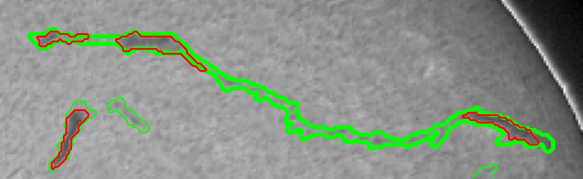
\includegraphics[width=\textwidth]{figuras/ejemplo_fragmentado.png}
\caption*{(a) Fragmentado con hueco real.}
\end{minipage}\hfill
\begin{minipage}[c]{0.38\textwidth}
\centering
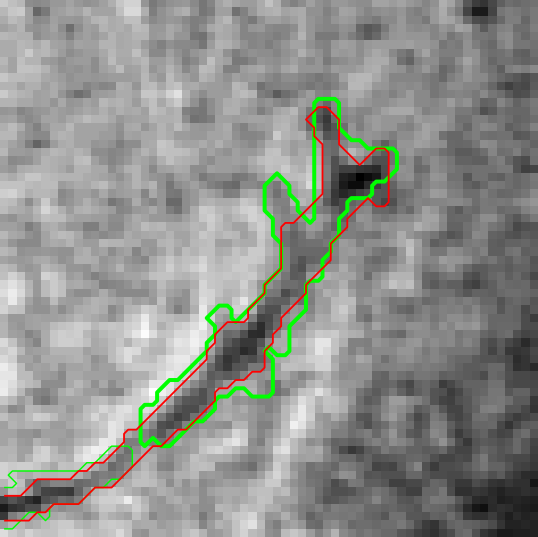
\includegraphics[width=\textwidth]{figuras/ejemplo_fusionado.png}
\caption*{(b) Fusionado.}
\end{minipage}
\caption{Dos errores típicos de segmentación sobre observaciones H-alfa de
GONG, con la referencia en verde y la predicción en rojo. (a) Un filamento
partido en varios trozos separados por huecos reales. (b) Dos filamentos de
la referencia (el pequeño, abajo a la izquierda, y el principal) unidos en
una única predicción.}
\label{fig:errores-ejemplo}
\end{figure}

% ------------------------------------------------------------
\section{El conjunto de datos MAGFiLO}
\label{sec:magfilo}
% ------------------------------------------------------------

MAGFiLO (\emph{Manually Annotated GONG Filaments in H-alpha Observations})
es un conjunto de datos de filamentos anotados manualmente sobre
observaciones H-alfa de GONG~\cite{ahmadzadeh2024}. Su versión 1.0 contiene
10\,244 filamentos anotados en 958 observaciones entre 2011 y 2022. Para cada filamento incluye la máscara de segmentación, la caja
contenedora mínima, la espina (la línea que recorre su eje principal) y la
quiralidad (el sentido de giro de su campo magnético, deducido de las
barbas; Sección~\ref{sec:filamentos}).

La anotación supuso más de 1\,000 horas-persona, con un proceso de
revisión doble ciego: cada observación fue anotada por hasta tres
anotadores independientes, y cada anotación, revisada después por
separado~\cite{ahmadzadeh2024}. El acuerdo entre anotadores sobre la
quiralidad se mide con el estadístico $\kappa$ de Cohen~\cite{cohen1960},
que compara el acuerdo observado con el que cabría esperar por azar
($\kappa=0$: acuerdo casual; $\kappa=1$: acuerdo perfecto). El valor
obtenido, $\kappa=0{,}66$, se considera un acuerdo
«sustancial»~\cite{ahmadzadeh2024}. Para las
máscaras, que son lo que se evalúa en este trabajo, el artículo no da una
medida de acuerdo; la estimamos en la Sección~\ref{sec:diagnostico}.

\paragraph{Subconjunto de la competición.} La competición usa solo las
máscaras de segmentación~\cite{kaggle2026}. El conjunto de entrenamiento
público está organizado por \emph{pares anotador--imagen}: cada imagen
aparece tantas veces como anotadores la hayan etiquetado, cada vez con su
propio conjunto de filamentos. La Tabla~\ref{tab:datos} resume sus
características.

\begin{figure}[ht]
\centering
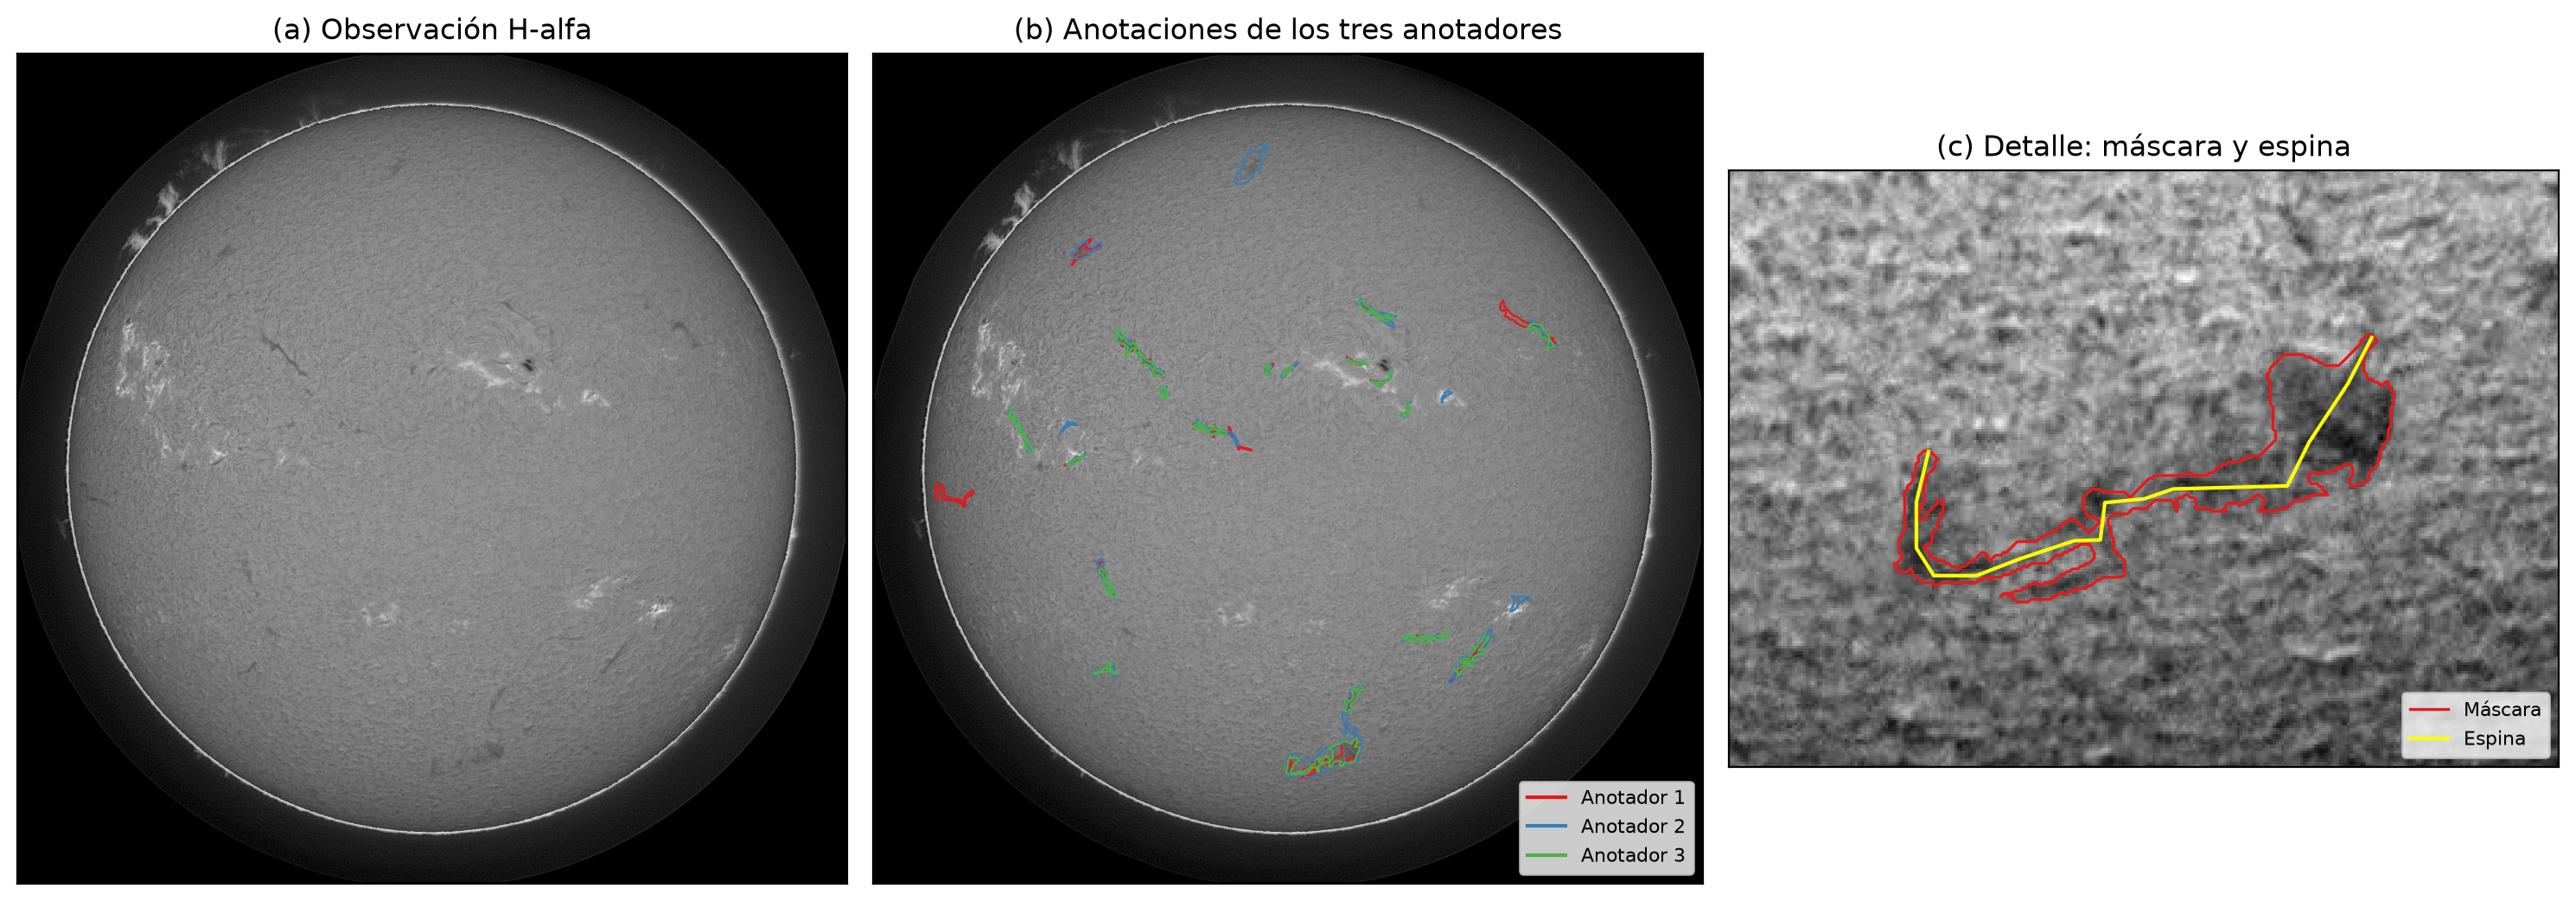
\includegraphics[width=\textwidth]{magfilo_ejemplo.png}
\caption{Una observación del conjunto de entrenamiento. (a) Imagen H-alfa
de disco completo. (b) Anotaciones de los tres anotadores que la
etiquetaron, una por color: coinciden en los filamentos grandes y difieren
en los pequeños y en la extensión de cada uno. (c) Detalle de un
filamento con su máscara y la espina anotada.}
\label{fig:magfilo}
\end{figure}

\begin{table}[ht]
\centering
\begin{tabular}{@{}lr@{}}
\toprule
Imágenes distintas & 707\\
Pares anotador--imagen & 1\,154\\
\quad imágenes con 1 / 2 / 3 anotadores & 411 / 145 / 151\\
Filamentos anotados (sumando anotadores) & 8\,199\\
Filamentos por par (media) & 7{,}1\\
Periodo & 2011--2022\\
Resolución & $2048\times2048$\\
\bottomrule
\end{tabular}
\caption{Conjunto de entrenamiento público de la competición, calculado a
partir del fichero de anotaciones.}
\label{tab:datos}
\end{table}

Las imágenes son de disco completo, de $2048\times2048$
píxeles~\cite{kaggle2026}. Las seis estaciones están representadas de forma equilibrada, entre 102 y
127 imágenes cada una. La distribución temporal no lo está: la mayoría de
las imágenes son de 2011--2017, y los años 2018--2022 aportan pocas
observaciones. Además, de un mismo día suele haber varias observaciones,
tomadas desde estaciones distintas, que muestran prácticamente el mismo
Sol. Este hecho obliga a separar entrenamiento y validación por fecha y
no por imagen, como se explica en el Capítulo~\ref{cap:metodologia}.

El conjunto de test es oculto. Solo se dispone de sus imágenes, y las
predicciones se evalúan en la plataforma.

% ------------------------------------------------------------
\section{La competición \emph{Solar Filament Segmentation Challenge 2026}}
\label{sec:competicion}
% ------------------------------------------------------------

El trabajo se enmarca en el \emph{Solar Filament Segmentation Challenge
2026}, una competición de Kaggle organizada dentro de la IEEE BigData Cup
2026 y patrocinada por el National Solar Observatory~\cite{kaggle2026}.
Se lanzó el 10 de julio de 2026 y el plazo de entrega final es el 15 de
noviembre de 2026.

\paragraph{Tarea.} Se pide generar una máscara de segmentación para cada
filamento \emph{individual}, que capture toda su extensión, incluidas las
estructuras finas como las barbas, y que incluya el menor número posible
de píxeles ajenos al filamento~\cite{kaggle2026}. Se trata, por tanto, de
un problema de \emph{segmentación de instancias} de una sola clase. El
envío es un fichero con una fila por filamento predicho, que contiene el
identificador de la imagen y la máscara codificada en RLE a resolución
original.

\paragraph{Métrica.} La métrica principal es la \emph{calidad
panóptica} (\emph{Panoptic Quality}, PQ)~\cite{kirillov2019}. Inicialmente
la competición usaba el coeficiente Dice, pero los organizadores lo
sustituyeron por PQ el 7 de agosto de 2026~\cite{kaggle2026}.

La métrica compara \emph{segmentos}. Un segmento es el conjunto de píxeles
que forman un único filamento, es decir, la máscara binaria de una
instancia, en la referencia, cada filamento anotado; en la predicción,
cada instancia que devuelve el modelo, que en este trabajo es una
componente conexa de la máscara predicha (Sección~\ref{sec:postproceso}).
Así, una imagen con siete filamentos tiene siete segmentos de referencia,
y el IoU entre dos segmentos se calcula sobre sus conjuntos de píxeles.

\begin{definicion}[{\cite{kirillov2019}}]
Sean $Y$ el conjunto de segmentos de referencia e $\hat Y$ el de segmentos
predichos. Un par $(y,\hat y)\in Y\times\hat Y$ es un \emph{verdadero
positivo} si $\operatorname{IoU}(y,\hat y)>0{,}5$, donde
\[
  \operatorname{IoU}(y,\hat y)=\frac{|y\cap\hat y|}{|y\cup\hat y|}.
\]
Los segmentos predichos sin pareja son \emph{falsos positivos} (FP) y los
de referencia sin pareja, \emph{falsos negativos} (FN). La calidad
panóptica es
\[
  \mathrm{PQ}=\frac{\sum_{(y,\hat y)\in \mathit{TP}}\operatorname{IoU}(y,\hat y)}
                   {|\mathit{TP}|+\tfrac12|\mathit{FP}|+\tfrac12|\mathit{FN}|}.
\]
\end{definicion}

El umbral $\operatorname{IoU}>0{,}5$ tiene una consecuencia importante. Si
los segmentos predichos no se solapan entre sí, cada segmento de
referencia puede emparejarse como mucho con uno predicho, y viceversa. El
emparejamiento es, por tanto, único y no requiere ningún algoritmo de
asignación~\cite{kirillov2019}. Además, PQ se factoriza como
\[
  \mathrm{PQ}=
  \underbrace{\frac{\sum_{\mathit{TP}}\operatorname{IoU}}{|\mathit{TP}|}}_{\mathrm{SQ}}
  \times
  \underbrace{\frac{|\mathit{TP}|}{|\mathit{TP}|+\tfrac12|\mathit{FP}|+\tfrac12|\mathit{FN}|}}_{\mathrm{RQ}},
\]
donde la \emph{calidad de segmentación} SQ es el IoU medio de los aciertos
y mide lo bien delimitados que están. La \emph{calidad de reconocimiento}
RQ mide, en cambio, cuántos filamentos se detectan, sin mirar cómo de bien.
Si llamamos \emph{precisión} a la fracción de segmentos predichos que son
aciertos, $P=|TP|/(|TP|+|FP|)$, y \emph{exhaustividad} a la fracción de
segmentos de referencia que se aciertan, $R=|TP|/(|TP|+|FN|)$, entonces
\[
  \mathrm{RQ}=\frac{2|TP|}{2|TP|+|FP|+|FN|}=\frac{2PR}{P+R},
\]
es decir, RQ es la media armónica de $P$ y $R$, la medida $F_1$ habitual
en detección~\cite{kirillov2019}. Es alta solo si el modelo encuentra la
mayoría de los filamentos ($R$ alta) sin inventar muchos ($P$ alta).

En la competición, $Y$ e $\hat Y$ contienen los segmentos de
\emph{todas} las imágenes. Es decir, se suman TP, FP, FN e IoU sobre todo
el conjunto antes de dividir, y no se promedia imagen a
imagen~\cite{kaggle2026}. Como unidad de evaluación se usa el par
anotador--imagen: las predicciones de una imagen se comparan por separado
con la anotación de cada anotador. Por ejemplo, si una imagen tiene tres
anotaciones, el mismo modelo se evalúa tres veces sobre esa imagen, una por
cada anotador, y cada comparación aporta sus propios TP, FP y FN. Así, la
evaluación no favorece a ningún anotador concreto, pero el desacuerdo entre
ellos se traslada directamente a la métrica.

Como referencia de escala, los organizadores consideran que un PQ superior a
$0{,}35$ es un resultado de gran valor~\cite{kaggle2026}, esta cifra coincide con el acuerdo entre expertos. Si se
comparan entre sí las anotaciones de distintos anotadores sobre una misma
imagen, con la misma métrica, se obtiene un PQ de aproximadamente $0{,}34$
(Sección~\ref{sec:techo-humano}). Un modelo que supere $0{,}35$ se parece,
por tanto, a cada anotador tanto como los anotadores se parecen entre sí. Es, por tanto, el umbral con el que conviene comparar nuestros resultados.

\paragraph{Rúbrica.} La clasificación en el \emph{leaderboard} es solo una
parte de la evaluación final~\cite{kaggle2026}:
\begin{itemize}
  \item \textbf{Comparación cuantitativa (70\,\%):} PQ y las
  distribuciones de Dice, de IoU y de relaciones uno-a-varios y
  varios-a-uno entre segmentos predichos y de referencia. Estas últimas
  penalizan la \emph{fragmentación} (un filamento predicho en varios
  trozos) y la \emph{fusión} (varios filamentos predichos como uno).
  \item \textbf{Comparación cualitativa (30\,\%):} la descripción del
  pipeline completo, la morfología aparente de las predicciones y la
  calidad del código.
\end{itemize}
El \emph{leaderboard} público se calcula con aproximadamente la mitad del
conjunto de test; la otra mitad solo la ven los organizadores.

% ------------------------------------------------------------
\section{Detección automática de filamentos: trabajos previos}
\label{sec:estado-arte}
% ------------------------------------------------------------

La detección automática de filamentos en imágenes H-alfa tiene una
trayectoria de más de dos décadas. Podemos distinguir dos etapas.

\paragraph{Métodos clásicos.} Los primeros métodos se basan en que los
filamentos son más oscuros que su entorno, y los extraen con umbrales,
operaciones morfológicas y reglas para descartar otras regiones oscuras.
Un ejemplo representativo es el de Bernasconi et
al.~\cite{bernasconi2005}, que detecta, sigue y caracteriza filamentos,
incluida su quiralidad a partir de las barbas. Estos métodos son
interpretables y rápidos, pero dependen de umbrales ajustados a mano,
son sensibles a las condiciones de observación y tienden a confundir
filamentos con manchas solares y otras regiones
oscuras~\cite{diercke2024}.

\paragraph{Aprendizaje profundo.} Con las redes convolucionales, el
problema se ha abordado como segmentación semántica o de instancias.
Zhu et al.~\cite{zhu2019} entrenan una U-Net~\cite{ronneberger2015} sobre
imágenes H-alfa con máscaras obtenidas de forma semiautomática. Diercke
et al.~\cite{diercke2024} proponen un método semisupervisado: un detector
YOLOv5 entrenado con cajas anotadas a mano genera etiquetas aproximadas
sobre el archivo de GONG, y con ellas entrenan una U-Net.

Un rasgo común de estos trabajos es la escasez de anotaciones manuales a
nivel de píxel: la mayoría entrena con máscaras obtenidas por
umbralización o por otros detectores, que heredan sus errores. MAGFiLO
cubre precisamente esta carencia~\cite{ahmadzadeh2024}. Sobre MAGFiLO,
Solomon et al.~\cite{solomon2025} proponen EdgeAttNet, una U-Net con
atención guiada por bordes en el cuello de botella, orientada a capturar
mejor las barbas, y la comparan con una U-Net estándar entrenada con
BCE + Dice.

Hasta donde conocemos, estos trabajos optimizan pérdidas de solapamiento
píxel a píxel y se evalúan con métricas de solapamiento (precisión,
exhaustividad, IoU). Ninguno incorpora restricciones topológicas al
entrenamiento ni al post-procesado. Tampoco se habían evaluado con una
métrica de instancias como PQ, que penaliza explícitamente la
fragmentación y la fusión. Este es el hueco que aborda este trabajo.

% ------------------------------------------------------------
\section{Dificultades del problema}
\label{sec:dificultades}
% ------------------------------------------------------------

Los propios organizadores señalan tres dificultades
principales~\cite{kaggle2026} (ítems 1 a 3), a las que añadimos dos más
(ítems 4 y 5):

\begin{enumerate}
  \item \textbf{Estructuras finas.} Las barbas tienen pocos píxeles de
  anchura y contraste débil. Son las primeras en perderse, y su
  orientación es justo la que aporta información física.
  \item \textbf{Ruido e imagen terrestre.} Distinguir el material del
  filamento de otras regiones oscuras (manchas, ruido, artefactos) no es
  trivial en observaciones afectadas por la atmósfera.
  \item \textbf{Continuidad estructural.} Los algoritmos tienden a
  devolver filamentos \emph{fragmentados} o a agrupar regiones oscuras
  cercanas en «islas», con resultados físicamente incoherentes.
\item \textbf{Desacuerdo entre anotadores.} Los anotadores no coinciden
  siempre en dónde empieza y acaba un filamento, ni en si dos trozos
  forman uno o dos filamentos. Esto fija un techo a lo que puede conseguir
  cualquier modelo frente a una anotación concreta. Lo cuantificamos con
  el PQ de un anotador frente a otro sobre la misma imagen, que es el
  techo humano de la métrica.
  \item \textbf{Desequilibrio de clases.} Los filamentos ocupan una
  fracción muy pequeña de cada imagen, de modo que una pérdida píxel a
  píxel está dominada por el fondo.
\end{enumerate}

Las dificultades 1 y 3 son, en el fondo, \emph{topológicas}. Si las
instancias se obtienen como componentes conexas de una máscara binaria, el
número de filamentos predichos es el número de componentes conexas, es decir,
el número de Betti $\beta_0$ de esa máscara. Un filamento partido en dos
aumenta $\beta_0$: un acierto se convierte en un falso negativo y en dos falsos
positivos, aunque falten solo unos pocos píxeles. Dos filamentos unidos por un
puente de píxeles hacen el error contrario. Una barba perdida, en cambio, apenas
cambia el IoU. Métricas como Dice o el propio IoU, que cuentan píxeles, son
poco sensibles a estos errores, mientras que PQ y la rúbrica los penalizan con
fuerza.

% ============================================================
% Capítulo 4 — Planteamiento
% ============================================================

\chapter{Planteamiento}
\label{cap:planteamiento}

Los capítulos anteriores han presentado las herramientas topológicas
(Capítulo~\ref{cap:fundamentos}) y el problema práctico
(Capítulo~\ref{cap:contexto}). Este capítulo explica cómo se combinan en
el trabajo. El punto de partida no es proponer mejoras a ciegas, sino
\emph{diagnosticar} primero qué errores comete un modelo de referencia
(Sección~\ref{sec:diagnostico}). Después se muestra que el post-proceso
habitual tiene una lectura topológica directa: las instancias que produce
son puntos de un diagrama de persistencia, y cada tipo de error deja en
ese diagrama una firma reconocible (Sección~\ref{sec:lectura-topologica}).
De esa lectura salen las hipótesis y las líneas de mejora del trabajo
(Sección~\ref{sec:estrategia}) y la forma de medir si una mejora funciona
(Sección~\ref{sec:medir}).

% ------------------------------------------------------------
\section{Diagnóstico de la baseline}
\label{sec:diagnostico}
% ------------------------------------------------------------

El modelo de referencia, o \emph{baseline}, es una U-Net entrenada con
BCE + Dice. Para obtener instancias se umbraliza su mapa de
probabilidades, se toman las componentes conexas y se descartan las de
área menor que un mínimo. Los detalles se describen en el
Capítulo~\ref{cap:metodologia}. Lo que interesa aquí es \emph{cómo} se
equivoca este modelo.

\subsection{Taxonomía de errores}

El PQ solo distingue entre aciertos, falsos positivos y falsos negativos.
Para decidir qué mejorar hace falta más detalle, así que se clasifica
cada filamento de referencia y cada predicción según cómo se relacionan
entre sí. Decimos que una predicción y un filamento de referencia están
\emph{relacionados} si su IoU es al menos $0{,}1$ o si uno cubre al menos
el 50\,\% del otro. El segundo criterio evita que un trozo pequeño de un
filamento largo, cuyo IoU es bajo porque la unión es grande, se cuente
como espurio en lugar de como fragmento. Con esta relación, cada
filamento de referencia no acertado, y cada predicción sin filamento, se
clasifica en uno de los tipos de la Tabla~\ref{tab:taxonomia}.

\begin{table}[ht]
\centering
\small
\begin{tabular}{@{}lp{9cm}@{}}
\toprule
Tipo & Descripción\\
\midrule
Perdido & Ninguna predicción relacionada.\\
Fragmentado (1:$n$) & Relacionado con varias predicciones, que son sus trozos.\\
Fusionado ($n$:1) & Su predicción relacionada lo está también con otros filamentos.\\
Mal delimitado & Una sola predicción relacionada, pero con $\mathrm{IoU}\le0{,}5$.\\
Espurio (predicción) & Predicción sin ningún filamento relacionado.\\
\bottomrule
\end{tabular}
\caption{Tipos de error considerados en el diagnóstico.}
\label{tab:taxonomia}
\end{table}

Tres de estos tipos son errores \emph{topológicos} en un sentido preciso:
cambian el número de componentes. Un filamento fragmentado en $n$ trozos
aporta $n$ componentes donde debería haber una; $n$ filamentos fusionados
aportan una donde debería haber $n$, y un espurio aporta una componente
que no existe en la referencia. En términos de la
Sección~\ref{sec:homologia}, son discrepancias locales en $\beta_0$. Los
perdidos y los mal delimitados, en cambio, no se deben a la conectividad
de la predicción, sino a su presencia o a su forma.

La relación anterior es más exigente que la de las gráficas oficiales de
la competición, que consideran relacionados una predicción y un filamento
en cuanto se solapan ($\mathrm{IoU}>0$). En el
Capítulo~\ref{cap:resultados} los tipos de error se cuentan con la
definición oficial, para que sean comparables con la rúbrica.

\subsection{Recuperabilidad}

Un error solo se puede corregir en el post-proceso si el mapa de
probabilidades contiene la señal necesaria. Para los perdidos y los
fragmentados se mide esa \emph{recuperabilidad}:
\begin{itemize}
  \item Para un filamento \emph{perdido}, se mira la probabilidad máxima
  en su interior. Si es muy baja, el modelo no lo vio, y ningún
  post-proceso lo recuperará. Si queda algo por debajo del umbral, la
  señal existe.
  \item Para un filamento \emph{fragmentado}, se calcula su
  \emph{collado}: el umbral más alto al que sus trozos quedan unidos por
  un camino dentro del filamento. Si el collado está justo por debajo del
  umbral, basta con bajarlo un poco para que los trozos se unan. Un
  collado de $0$ indica un hueco real en la predicción, que ningún umbral
  cierra.
\end{itemize}
El collado es una noción topológica: es el valor del punto de silla en
el que se funden las componentes de los trozos, es decir, el valor de
\emph{muerte} de las componentes más jóvenes en la filtración de
superniveles restringida al filamento (Sección~\ref{sec:persistencia}).
La Sección~\ref{sec:lectura-topologica} desarrolla esta conexión.

\subsection{Dónde falla el modelo}

Este diagnóstico se hizo con una primera versión de la baseline,
entrenada antes de fijar el protocolo del
Capítulo~\ref{cap:metodologia}. Sus cifras no son comparables con las
del Capítulo~\ref{cap:resultados}, pero sirvieron para decidir la
estrategia. El análisis sobre la validación muestra cuatro patrones:
\begin{itemize}
  \item La exhaustividad cae en los filamentos pequeños (25\,\%), en los
  cercanos al borde del disco solar (el limbo, 15\,\%) y en los que ningún otro anotador marca
  (14\,\%, frente al 68\,\% de los que marcan todos).
  \item Muchos filamentos sí se detectan, pero los elimina el filtro de
  área mínima: 203 filamentos de validación se pierden solo por él.
  \item Los espurios tienen casi la misma confianza que los aciertos
  (probabilidad máxima mediana de $0{,}917$ frente a $0{,}933$), así que
  la confianza por sí sola no los separa.
  \item Aproximadamente el 54\,\% de los espurios los marca otro
  anotador de la misma imagen. Más que errores del modelo, son
  desacuerdos entre anotadores.
\end{itemize}
Los tres primeros patrones son los que motivan este trabajo, y los dos
primeros están relacionados. Parte de la exhaustividad que se pierde en
los filamentos pequeños se debe al post-proceso: el filtro de área
elimina filamentos reales por su tamaño, y el umbral deja fuera los que
el modelo detecta con poca confianza. El tercer patrón añade que la
confianza tampoco sirve para distinguir los espurios. Hace falta, por
tanto, otro criterio para decidir qué componentes conservar, y la
persistencia es un candidato para los casos en los que fallan el área y
el umbral (Sección~\ref{sec:lectura-topologica}). Las pérdidas en el
limbo y en los filamentos que marca un solo anotador dependen más de la
imagen y de la anotación, y son más difíciles de corregir desde el
post-proceso.

\subsection{El techo humano}
\label{sec:techo-humano}

Comparando entre sí las anotaciones de las imágenes con varios
anotadores, con el mismo PQ, se obtiene un acuerdo humano de
$\mathrm{PQ}\approx0{,}34$. Esa primera baseline, comparada con cada
anotador, obtiene $\approx0{,}38$. El modelo se parece más a cada
anotador que los anotadores entre sí, porque aprende una especie de
consenso. Este dato es esencial para interpretar cualquier resultado: con
referencias tan ruidosas, un PQ cercano a $1$ no es alcanzable, y parte
de los «errores» son desacuerdos entre expertos.

% ------------------------------------------------------------
\section{Lectura topológica del post-proceso}
\label{sec:lectura-topologica}
% ------------------------------------------------------------

\subsection{Instancias y diagrama de persistencia}

Sea $p$ el mapa de probabilidades que produce la red. Dado un umbral
$t$, el post-proceso toma el conjunto de supernivel
\[
  X_t=\{x : p(x)>t\}
\]
y declara que cada componente conexa de $X_t$ es un filamento. Las
componentes se calculan con 8-conectividad, es decir, con la
construcción T (Observación~\ref{obs:conectividad}), para no fragmentar
artificialmente las barbas. Antes del filtro de área, el número de
instancias predichas es, por tanto, $\beta_0(X_t)$.

En lugar de mirar un solo umbral, podemos considerar la filtración de
superniveles completa, con $t$ bajando de $1$ a $0$, y su diagrama de
persistencia en dimensión $0$ (Sección~\ref{sec:persistencia}). Es la
situación de la Figura~\ref{fig:elder} con el paisaje del revés: en vez
de subir el nivel del agua, se baja el umbral. Cada componente
\emph{nace} en un máximo local de $p$, con valor $b$, y \emph{muere} en
$d<b$, cuando se funde en un collado con otra componente nacida antes,
según la regla del mayor. La componente del máximo global no muere
nunca, y le asignamos $d=-\infty$.

\begin{proposicion}
\label{prop:instancias}
Supongamos que los valores de $p$ son distintos dos a dos. Para todo
umbral $t$, el número de instancias de la baseline antes del
filtro de área es
\[
  \beta_0(X_t)=\#\{(b,d)\in\operatorname{Dgm}_0 : b>t\ge d\}.
\]
\end{proposicion}

\begin{proof}[idea]
Cada componente de $X_t$ contiene un único máximo más antiguo, el de
valor más alto. Por la regla del mayor, la componente que nació en ese
máximo sigue viva en $t$: ya ha nacido, porque $b>t$, y todavía no ha
muerto, porque cualquier componente con la que se haya fundido era más
joven, así que $d\le t$. Las demás componentes nacidas dentro de esa
región ya han muerto al fundirse con ella, con $d>t$. Hay, por tanto, una
biyección entre las componentes de $X_t$ y los puntos con $b>t\ge d$.
Es el caso de dimensión $0$ del resultado general según el cual
$\beta_p$ de un espacio de la filtración es el número de intervalos del
código de barras que lo contienen~\cite[§VII.1]{edelsbrunner2010}.
\end{proof}

Es decir, umbralizar en $t$ equivale a quedarse con los puntos del
diagrama en el cuadrante $\{b>t,\ d\le t\}$, y el post-proceso deja de
ser un ajuste de dos números para convertirse en una decisión sobre qué
puntos del diagrama convertir en instancias.

\begin{ejemplo}
\label{ej:perfil}
Sea $p$ el perfil de probabilidad a lo largo de una línea de la imagen
que toma los valores
$0{,}05,\ 0{,}90,\ 0{,}45,\ 0{,}80,\ 0{,}10,\ 0{,}70,\ 0{,}05$
(Figura~\ref{fig:perfil}). Los dos primeros máximos, $A$ y $B$,
pertenecen al mismo filamento, partido por una bajada de la
probabilidad; el tercero, $C$, es una mancha sin filamento debajo. Al
bajar el umbral:
\begin{itemize}
  \item En $t=0{,}90$ nace la componente de $A$; en $t=0{,}80$, la de
  $B$; en $t=0{,}70$, la de $C$.
  \item En $t=0{,}45$ se supera el collado entre $A$ y $B$, y sus
  componentes se funden. Muere la más joven, la de $B$.
  \item En $t=0{,}10$ se supera el collado entre $B$ y $C$, ya dentro de
  la componente de $A$, y muere la de $C$.
\end{itemize}
El diagrama es $\{(0{,}90,-\infty),\ (0{,}80,0{,}45),\ (0{,}70,0{,}10)\}$.
Con $t=0{,}5$, los tres puntos cumplen $b>t\ge d$, y la baseline produce
tres instancias: el filamento aparece partido en dos y, además, hay un
espurio.
\end{ejemplo}

\begin{figure}[ht]
\centering
\begin{tikzpicture}
  % --- perfil: 0,9 cm por posición, 3,6 cm por unidad de probabilidad ---
  \begin{scope}[x=0.9cm, y=3.6cm]
    \draw[->] (-0.3,0) -- (6.5,0);
    \draw[->] (0,-0.05) -- (0,1.08) node[above] {\small $p$};
    \fill[blue!12] (0,0) -- (0,0.05) -- (1,0.90) -- (2,0.45) -- (3,0.80)
          -- (4,0.10) -- (5,0.70) -- (6,0.05) -- (6,0) -- cycle;
    \draw[thick] (0,0.05) -- (1,0.90) -- (2,0.45) -- (3,0.80) -- (4,0.10)
          -- (5,0.70) -- (6,0.05);
    \draw[dashed, gray] (0,0.5) -- (6.3,0.5) node[right] {\small $t=0{,}5$};
    \fill[red!80!black] (1,0.90) circle (2.2pt) node[above=2pt] {\small $A$};
    \fill[green!50!black] (3,0.80) circle (2.2pt) node[above=2pt] {\small $B$};
    \fill[orange!90!black] (5,0.70) circle (2.2pt) node[above=2pt] {\small $C$};
    \node[below, font=\small] at (2,0.45) {$0{,}45$};
    \node[right, font=\small] at (4.05,0.08) {$0{,}10$};
    \draw[thick, gray] (0.6,-0.17) -- (3.4,-0.17);
    \node[below, font=\small] at (2,-0.17) {filamento};
    \draw[thick, gray] (4.6,-0.17) -- (5.4,-0.17);
    \node[below, font=\small] at (5,-0.17) {espurio};
  \end{scope}
  % --- código de barras: t de 1 (izquierda) a 0 (derecha) ---
  \begin{scope}[xshift=7.6cm, x=4cm, y=0.55cm]
    \draw[->] (0,0) -- (1.08,0) node[right] {\small $t$};
    \foreach \t/\l in {0/1, 0.5/0{,}5, 1/0} {
      \draw (\t,0.12) -- (\t,-0.12) node[below] {\small $\l$};
    }
    % A: de 0,90 a -infinito
    \draw[line width=3pt, red!80!black] (0.10,4) -- (1.0,4);
    \draw[->, red!80!black, thick] (0.98,4) -- (1.06,4);
    % B: de 0,80 a 0,45
    \draw[line width=3pt, green!50!black] (0.20,2.8) -- (0.55,2.8);
    % C: de 0,70 a 0,10
    \draw[line width=3pt, orange!90!black] (0.30,1.6) -- (0.90,1.6);
    \node[left, font=\small] at (0.08,4) {$A$};
    \node[left, font=\small] at (0.18,2.8) {$B$};
    \node[left, font=\small] at (0.28,1.6) {$C$};
    \draw[dashed, gray] (0.5,0.4) -- (0.5,4.6);
  \end{scope}
\end{tikzpicture}
\caption{Izquierda: perfil de probabilidad del
Ejemplo~\ref{ej:perfil}. Los máximos $A$ y $B$ son dos trozos del mismo
filamento y $C$ es una mancha espuria. Derecha: código de barras $H_0$ de
la filtración de superniveles, con el umbral $t$ bajando de izquierda a
derecha. La línea discontinua en $t=0{,}5$ corta las tres barras: la
baseline produce tres instancias. Ilustración propia.}
\label{fig:perfil}
\end{figure}

\subsection{La firma de cada error}

Cada tipo de error de la Tabla~\ref{tab:taxonomia} deja una firma
reconocible en el diagrama (Tabla~\ref{tab:firmas}).

\begin{table}[ht]
\centering
\small
\begin{tabular}{@{}lp{10.5cm}@{}}
\toprule
Error & Firma en el diagrama $H_0$ de superniveles\\
\midrule
Fragmentado & Varios puntos del cuadrante nacidos dentro del mismo
filamento. La muerte $d$ de los más jóvenes es el collado entre trozos:
si está justo por debajo de $t$, el hueco es recuperable bajando el
umbral.\\
Fusionado & Los máximos de dos filamentos se unen en un collado por
encima de $t$. El más joven muere antes de llegar al umbral ($d>t$), y
en el cuadrante queda un solo punto para los dos.\\
Perdido & Ningún punto con $b>t$ dentro del filamento. Si hay uno con
$b$ algo menor que $t$, la señal existe pero queda por debajo del
umbral.\\
Espurio & Un punto del cuadrante sin filamento debajo. Su persistencia
depende del entorno: es baja si es un pequeño relieve sobre una zona de
probabilidad intermedia, y alta si es una mancha aislada sobre un fondo
cercano a $0$.\\
\bottomrule
\end{tabular}
\caption{Firma de cada tipo de error en el diagrama de persistencia $H_0$
de la filtración de superniveles, para un umbral $t$.}
\label{tab:firmas}
\end{table}

En el Ejemplo~\ref{ej:perfil}, el filamento fragmentado aparece como los
puntos de $A$ y $B$, y el collado que los separa es la muerte de $B$,
$d=0{,}45$, a solo $0{,}05$ por debajo del umbral: bajando el umbral a
$0{,}44$ los dos trozos se unirían. El espurio $C$ ilustra el segundo
caso de la última fila: está aislado sobre un fondo bajo, de modo que su
persistencia, $0{,}70-0{,}10=0{,}60$, es mayor que la de $B$,
$0{,}80-0{,}45=0{,}35$, que es un trozo de un filamento real. La
persistencia mide la robustez de una componente frente al umbral, no si
corresponde a un filamento.

\subsection{Área frente a persistencia}

El filtro de área de la baseline es un criterio \emph{geométrico}:
descarta las componentes de $X_t$ pequeñas, sea cual sea su punto en el
diagrama. Dos componentes con el mismo par $(b,d)$ pueden tener áreas muy
distintas, así que el área no es una función del diagrama.

La persistencia ofrece un criterio \emph{topológico}, con una
justificación teórica. Por el teorema de estabilidad
(Sección~\ref{sec:distancias}), si la predicción cambia en cada píxel
como mucho en $\varepsilon$, los puntos del diagrama se desplazan como
mucho $\varepsilon$, y solo pueden aparecer o desaparecer los de
persistencia menor que $2\varepsilon$. Las componentes poco persistentes
son, por tanto, las que dependen de pequeñas fluctuaciones de la
predicción, y las muy persistentes, las que sobreviven a ellas. Si los
filamentos pequeños que elimina el filtro de área son robustos y los
espurios no, un filtro por persistencia los separaría mejor.

El Ejemplo~\ref{ej:perfil} muestra también el límite de esta idea: un
espurio aislado sobre un fondo bajo es muy persistente. Cuál de los dos
casos de la última fila de la Tabla~\ref{tab:firmas} domina en la
práctica es una pregunta empírica, que responde la
Sección~\ref{sec:res-e2}.

\begin{observacion}
La filtración de superniveles de $p$ y la de su \emph{logit}
$z=\log\frac{p}{1-p}$ son la misma, reparametrizada: como la sigmoide es
estrictamente creciente, $\{p>t\}=\{z>\operatorname{logit}(t)\}$, y los
diagramas tienen los mismos emparejamientos. Lo que cambia son los
valores $b$ y $d$ y, con ellos, la persistencia $b-d$: la sigmoide
comprime los valores cercanos a $0$ y a $1$, de modo que una diferencia
pequeña en $p$ puede ser grande en $z$. Por eso un umbral de
persistencia $\tau$ solo tiene sentido referido a una escala. En este
trabajo la persistencia se mide sobre $p$, para que $\tau$ se interprete
en unidades de probabilidad.
\end{observacion}

% ------------------------------------------------------------
\section{Hipótesis y estrategia}
\label{sec:estrategia}
% ------------------------------------------------------------

Del diagnóstico y de la lectura topológica se derivan cuatro líneas de
mejora, cada una dirigida a un tipo de error
(Tabla~\ref{tab:estrategia}). Se ordenan de menor a mayor coste: primero
las que no requieren reentrenar.

\begin{table}[ht]
\centering
\footnotesize
\begin{tabular}{@{}lllc@{}}
\toprule
Línea & Error al que apunta & Reentrena & Estado\\
\midrule
E1. Umbral y área mínima & Espurios pequeños & No & Hecha\\
E2. Post-proceso por persistencia & Fragmentación, espurios & No & Hecha\\
E3. Pérdidas (IoU, clDice, Topograph) & Espurios, fragmentación, barbas & Sí & Hecha\\
E4. Etiquetas multianotador & Desacuerdo entre anotadores & Sí & Planteada\\
\bottomrule
\end{tabular}
\caption{Líneas de mejora, error al que apunta cada una y si se ha
desarrollado en este trabajo.}
\label{tab:estrategia}
\end{table}

\paragraph{E1. Ajuste del post-proceso clásico.} Se ajustan el umbral $t$
y el área mínima de las componentes. Es la mejora más barata y sirve de
segunda referencia para las demás. En el lenguaje de la sección
anterior, el umbral elige el cuadrante del diagrama y el área mínima
filtra sus puntos con un criterio geométrico.

\paragraph{E2. Post-proceso basado en persistencia.} Sustituye el
criterio geométrico por uno topológico. Parte de $X_u$, para un umbral
$u$, y aplica dos operaciones:
\begin{itemize}
  \item \emph{Filtro por persistencia.} Se conserva una componente de
  $X_u$ solo si contiene un máximo con persistencia $b-d\ge\tau$. En el
  Ejemplo~\ref{ej:perfil}, con $\tau=0{,}5$ se conservarían las
  componentes de $A$ y de $C$, y se eliminaría la de $B$.
  \item \emph{Fusión por collado.} Las componentes conservadas que se
  unen en $X_{u-\delta}$, es decir, cuyo collado está a menos de $\delta$
  por debajo del umbral, se cuentan como una sola instancia, sin añadir
  píxeles. Es la operación dirigida a los fragmentados recuperables, a
  costa de arriesgarse a crear fusiones. En el ejemplo, si
  $\tau\le0{,}35$, de modo que $B$ se conserva, y $\delta>0{,}05$, las
  componentes de $A$ y $B$ formarían una sola instancia.
\end{itemize}
El filtro se aplica antes de la fusión, de modo que un trozo poco
persistente se elimina aunque esté cerca de otro robusto. También se
estudia una variante, B2+P, que combina ambos criterios: conserva una
componente si su área supera el mínimo \emph{o} si su persistencia
supera $\tau$. Los parámetros se ajustan en validación.

Para el filtro no hace falta construir el diagrama completo. En
morfología matemática, los \emph{$h$-máximos} de una
imagen son los máximos regionales que sobresalen al menos $h$ por
encima del collado más alto que los une a un máximo
mayor~\cite{soille2003}. Esa altura es exactamente la persistencia
$b-d$ que asigna la regla del mayor, así que los $h$-máximos con
$h=\tau$ son los nacimientos de los puntos con $b-d\ge\tau$. Se ha
comprobado sobre imágenes sintéticas que la selección coincide con la
del diagrama calculado con \emph{union-find}
(Sección~\ref{sec:persistencia-eficiente}). En ambos casos el coste es
casi lineal en el número de píxeles, despreciable frente a la
inferencia.

\paragraph{E3. Pérdidas con sesgo topológico.} El post-proceso solo
puede trabajar con la señal que el modelo ya produce. Para los
fragmentados con hueco real, para los espurios muy seguros y para las
barbas perdidas hay que cambiar lo que aprende la red. Se comparan tres
alternativas a Dice:
\begin{itemize}
  \item \emph{IoU}, como control: es otra pérdida de solapamiento, sin
  sesgo topológico.
  \item \emph{clDice}~\cite{shit2021}, que mide el solapamiento de los
  esqueletos (Sección~\ref{sec:dice-cldice}). Premia la continuidad de
  las estructuras alargadas, lo que debería reducir la fragmentación y
  mejorar la detección de las barbas.
  \item \emph{Topograph}~\cite{lux2025}, que compara las componentes de
  la predicción binarizada y de la referencia mediante el grafo
  combinado y penaliza solo las regiones críticas, las que cambian la
  topología (Sección~\ref{sec:topograph}). Actúa durante el
  entrenamiento sobre los mismos errores que la Tabla~\ref{tab:firmas}
  lee en el diagrama: una componente espuria, un filamento partido o dos
  filamentos fusionados son discrepancias en el grafo combinado. La
  diferencia es que Topograph trabaja sobre un único umbral, el de la
  binarización ($p>0{,}5$), mientras que el post-proceso elige el
  umbral y puede mirar el diagrama completo.
\end{itemize}

\paragraph{E4. Estrategias de etiquetas.} Con varias anotaciones por
imagen, se comparan tres formas de construir la etiqueta de
entrenamiento: cada anotación como un ejemplo independiente (la opción
de la baseline), la media de las anotaciones como etiqueta blanda, y los
filamentos marcados por la mayoría de anotadores. La referencia de
evaluación no cambia con la estrategia: siempre se evalúa contra cada
anotación original.

\paragraph{Hipótesis.} Las líneas anteriores concretan cuatro hipótesis,
que el Capítulo~\ref{cap:resultados} contrasta:
\begin{enumerate}
  \item[H1.] Los errores dominantes se deben a componentes que sobran o
  que faltan, por lo que un filtro sobre las componentes (E1) mejora
  mucho el PQ.
  \item[H2.] La persistencia separa los filamentos pequeños de los
  espurios mejor que el área, y la fusión por collado repara parte de
  los fragmentados (E2).
  \item[H3.] Una pérdida que penaliza las regiones topológicamente
  críticas reduce las componentes espurias y la fragmentación sin
  necesidad de post-proceso (E3, Topograph).
  \item[H4.] Una pérdida que premia la continuidad del esqueleto mejora
  la detección de las barbas (E3, clDice).
\end{enumerate}

\paragraph{Alcance.} Este trabajo desarrolla las líneas E1, E2 y E3,
cuyos resultados se presentan en el Capítulo~\ref{cap:resultados}. La
línea E4 queda planteada y se recoge como trabajo futuro en el
Capítulo~\ref{cap:conclusiones}.

% ------------------------------------------------------------
\section{Cómo medir una mejora}
\label{sec:medir}
% ------------------------------------------------------------

Una mejora del PQ global puede esconder que se arreglan unos filamentos
y se rompen otros. Por eso cada versión se evalúa de tres formas:
\begin{enumerate}
  \item \textbf{Métrica oficial:} PQ global, con SQ y RQ, y las
  distribuciones de la rúbrica (IoU, Dice y relaciones 1:$n$ y $n$:1).
  \item \textbf{Tipos de error:} cuántos filamentos quedan partidos,
  unidos o sin detectar, y cuántas predicciones no tocan ningún
  filamento. Los dos primeros miden los errores de estructura, las
  discrepancias locales en $\beta_0$, y los dos últimos, los errores de
  presencia. Se añade una medida específica de las barbas.
  \item \textbf{Separación ajuste--reporte:} todas las decisiones (época,
  umbrales, parámetros del post-proceso) se toman en una mitad de la
  validación y la cifra se reporta en la otra, para no inflar los
  resultados.
\end{enumerate}
El protocolo concreto se detalla en el Capítulo~\ref{cap:metodologia}.

% ============================================================
% Capítulo 5 — Metodología
% ============================================================

\chapter{Metodología}
\label{cap:metodologia}

Este capítulo describe el protocolo común a todos los experimentos: cómo
se parten los datos, cómo se entrena y se elige cada modelo, cómo se
obtienen las instancias y cómo se evalúan. Todas las ejecuciones siguen
las mismas reglas, fijadas antes de empezar a comparar. Así, cualquier
diferencia entre dos resultados se debe a la pieza que cambia (la
pérdida, el post-proceso o los hiperparámetros) y no al protocolo. Cada
una de las dos primeras corresponde a una de las líneas de mejora de la
Sección~\ref{sec:estrategia}, y cada medida de la evaluación, a un tipo
de error de la Sección~\ref{sec:diagnostico}. El código está disponible
en \url{https://github.com/AgustinG-git/tfm-filamentos}
(Apéndice~\ref{ap:codigo}).

% ------------------------------------------------------------
\section{Datos y partición}
\label{sec:particion}
% ------------------------------------------------------------

Se usa el conjunto de entrenamiento de la competición, con las
anotaciones de MAGFiLO~\cite{ahmadzadeh2024,kaggle2026}. El conjunto de
test no tiene anotaciones públicas y solo se usa para enviar
predicciones al \emph{leaderboard}.

\paragraph{Partición por días.} Las imágenes de un mismo día son casi
idénticas: el Sol apenas cambia en unas horas. Si una imagen de un día
estuviera en entrenamiento y otra del mismo día en validación, el modelo
se evaluaría sobre algo que ya ha visto. Por eso la partición se hace por
\emph{fecha}: ningún día aparece en dos subconjuntos. Se reserva el
20\,\% de los días para validación, y estos se dividen a su vez en dos
mitades, $A$ y $B$ (Tabla~\ref{tab:split}). La partición se genera una
sola vez, con semilla fija, y se guarda junto al código.

Como todas las anotaciones de una imagen comparten fecha, una misma
imagen nunca aparece en dos subconjuntos, ni siquiera anotada por
anotadores distintos. En cambio, la partición no separa por anotador: de
los 37 anotadores, todos los de validación salvo uno aparecen también en
entrenamiento. Separar por anotador mediría la generalización a
anotadores nuevos, que no es el objetivo del trabajo; aquí se busca
generalizar a días no vistos, con anotaciones del mismo proyecto.

\begin{table}[ht]
\centering
\begin{tabular}{@{}lrrr@{}}
\toprule
Subconjunto & Días & Imágenes & Pares anotador--imagen\\
\midrule
Entrenamiento & 524 & 561 & 920\\
Validación $A$ & 66 & 72 & 113\\
Validación $B$ & 66 & 74 & 121\\
\bottomrule
\end{tabular}
\caption{Partición de los datos. La unidad de evaluación es el par
anotador--imagen (Sección~\ref{sec:competicion}).}
\label{tab:split}
\end{table}

\paragraph{Ajuste en $A$, reporte en $B$.} Toda decisión se toma en
$A$: la época del modelo, los parámetros del post-proceso y los
hiperparámetros. La cifra que se reporta es la de $B$, que no interviene
en ninguna decisión. Si se eligiera en el mismo conjunto en el que se
mide, la cifra estaría inflada: entre muchas variantes, alguna sale
mejor por azar.

\paragraph{Preprocesado.} Las imágenes H-alfa son de un canal y
$2048\times2048$ píxeles. Para entrenar se reducen a $512\times512$
(interpolación por área), se replica el canal tres veces y se
normalizan con la media y la desviación de ImageNet~\cite{deng2009},
porque el codificador viene preentrenado en ese conjunto. No se usan
aumentos de datos.

\paragraph{Etiquetas.} Cada anotación es un ejemplo de entrenamiento
independiente: una imagen con tres anotadores aporta tres pares
(imagen, máscara). La máscara de un par es la unión de los filamentos de
ese anotador, reducida a $512\times512$. La referencia de evaluación,
en cambio, son siempre las anotaciones originales, una por una y a
resolución completa.

% ------------------------------------------------------------
\section{Modelo y entrenamiento}
\label{sec:entrenamiento}
% ------------------------------------------------------------

El modelo es una U-Net~\cite{ronneberger2015} con codificador
ResNet-34~\cite{he2016} preentrenado en ImageNet, de la biblioteca
\emph{Segmentation Models PyTorch}~\cite{iakubovskii2019}. Produce un
mapa de probabilidades $p$ de una sola clase (filamento) a
$512\times512$.

Salvo en el ajuste de la Sección~\ref{sec:ajuste-hp}, todas las
ejecuciones usan la misma configuración: 30 épocas, lotes de 8,
optimizador AdamW~\cite{loshchilov2019} con tasa de aprendizaje
$3\cdot10^{-4}$ y \emph{weight decay} $10^{-4}$, y tasa de aprendizaje
con decaimiento coseno. La red se ejecuta en precisión mixta, pero las
pérdidas se calculan siempre en \texttt{float32}: en \texttt{float16}
las sumas de clDice sobre un lote (unos $2\cdot10^6$ píxeles) desbordan.
La semilla es 42; la baseline y Topograph se repiten además con la
semilla 43.

\paragraph{Selección de la época.} Al final de cada época se evalúa el
modelo en $A$ y se guarda el mejor. El criterio es fijo para todas las
versiones: PQ global a $512\times512$, con umbral $0{,}5$ y sin filtro
de área. En el lenguaje de la Sección~\ref{sec:lectura-topologica}, las
instancias evaluadas son las componentes de $X_{0{,}5}$, es decir, los
puntos del diagrama con $b>0{,}5\ge d$
(Proposición~\ref{prop:instancias}). Se usa este post-proceso mínimo a
propósito: si la época se eligiera con el post-proceso de cada versión,
la comparación entre pérdidas mezclaría dos efectos.

% ------------------------------------------------------------
\section{Pérdidas}
\label{sec:perdidas}
% ------------------------------------------------------------

Todas las pérdidas incluyen BCE, con peso $0{,}5$, y se obtienen
cambiando una sola pieza respecto a la baseline
(Tabla~\ref{tab:perdidas}). IoU se definió en la
Sección~\ref{sec:competicion}, Dice y clDice en la
Sección~\ref{sec:dice-cldice} y Topograph en la
Sección~\ref{sec:topograph}; aquí solo se fijan los pesos. IoU sirve de
control sin sesgo topológico; clDice añade un sesgo hacia la
continuidad del esqueleto, y Topograph, un sesgo hacia la topología de
las componentes.

\begin{table}[ht]
\centering
\begin{tabular}{@{}ll@{}}
\toprule
Nombre & Pérdida\\
\midrule
Baseline & $0{,}5\,\mathrm{BCE}+0{,}5\,\mathrm{Dice}$\\
IoU & $0{,}5\,\mathrm{BCE}+0{,}5\,\mathrm{IoU}$\\
clDice & $0{,}5\,\mathrm{BCE}+0{,}25\,\mathrm{Dice}+0{,}25\,\mathrm{clDice}$\\
IoU+clDice & $0{,}5\,\mathrm{BCE}+0{,}25\,\mathrm{IoU}+0{,}25\,\mathrm{clDice}$\\
clDice sin Dice & $0{,}5\,\mathrm{BCE}+0{,}5\,\mathrm{clDice}$\\
\midrule
\dots{} + Topograph & la anterior $+\,\alpha\,\mathcal{L}_{\mathrm{Topo}}$, $\alpha=0{,}04$\\
\bottomrule
\end{tabular}
\caption{Pérdidas comparadas. Cada una de las cinco primeras se entrena
también con el término de Topograph.}
\label{tab:perdidas}
\end{table}

\paragraph{clDice.} Se usa el esqueleto blando de Shit et
al.~\cite{shit2021}, con 10 iteraciones de erosión.

\paragraph{Topograph.} Se usa la implementación oficial~\cite{lux2025},
con 8-conectividad, la misma que el post-proceso. Tres decisiones fijan
cómo se añade:
\begin{itemize}
  \item \emph{Peso.} Con un modelo ya entrenado, el término de
  Topograph es unas 27 veces mayor que BCE+Dice. Con $\alpha=0{,}04$
  ambos pesan lo mismo. El valor se fija así y no se ajusta en las
  comparaciones de pérdidas.
  \item \emph{Calentamiento.} Con un modelo sin entrenar, la predicción
  tiene cientos de regiones críticas por imagen y el término no aporta
  una señal útil. Por eso Topograph se activa a partir de la sexta
  época; en las cinco primeras $\alpha=0$.
  \item \emph{Binarización.} El grafo combinado se construye a partir de
  una predicción binaria, mientras que la red produce probabilidades. La
  implementación oficial binariza internamente tomando en cada píxel la
  clase más probable (\emph{argmax}). La salida de un canal se le pasa
  como dos canales, $(0, z)$, con $z$ el \emph{logit}, de modo que la
  clase predicha es «filamento» si y solo si $z>0$, es decir, si
  $p>0{,}5$. La binarización solo sirve para decidir qué regiones son
  críticas; el gradiente llega a la red a través de las probabilidades
  de los píxeles de esas regiones (Sección~\ref{sec:topograph}).
\end{itemize}
Topograph actúa, por tanto, sobre las componentes de $X_{0{,}5}$ y de su
complemento: el mismo conjunto de supernivel con el que se elige la
época y el que la Sección~\ref{sec:lectura-topologica} lee en el
diagrama.

% ------------------------------------------------------------
\section{Post-proceso}
\label{sec:postproceso}
% ------------------------------------------------------------

Las instancias se obtienen del mapa de probabilidades $p$ a
$512\times512$. Los cuatro post-procesos del trabajo comparten el mismo
esquema: se umbraliza el mapa, $X_t=\{p>t\}$, se toma cada componente
8-conexa de $X_t$ como candidata y se decide cuáles conservar. En la
lectura de la Sección~\ref{sec:lectura-topologica}, las candidatas son
los puntos del diagrama $H_0$ de superniveles vivos en $t$, y cada
post-proceso es una regla distinta para decidir cuáles de ellos
convertir en instancias.

Para una componente $C$ de $X_t$, sean $|C|$ su área en píxeles,
$D_C$ el conjunto de puntos de $\operatorname{Dgm}_0(p)$ que nacen en
un máximo de $p$ situado dentro de $C$, y
\[
  \pi(C)=\max_{(b,d)\in D_C}\,(b-d)
\]
la mayor persistencia de esos máximos. El diagrama es el de
la filtración de superniveles de $p$ en toda la imagen, no solo por
encima de $t$, de modo que la muerte $d$ puede ser menor que $t$. La
Tabla~\ref{tab:postprocesos} recoge la regla de cada post-proceso.

\begin{table}[ht]
\centering
\small
\begin{tabular}{@{}llll@{}}
\toprule
Post-proceso & Se conserva $C$ si & Fusión & Parámetros y rangos\\
\midrule
B1 & siempre & no & $t\in[0{,}2,\,0{,}9]$\\
B2 & $|C|\ge a$ & no & $t\in[0{,}2,\,0{,}9]$, $a\in[0,\,300]$\\
E2 & $\pi(C)\ge\tau$ & sí, con $\delta$ & $t\in[0{,}2,\,0{,}9]$, $\tau\in[0{,}01,\,0{,}5]$, $\delta\in[0,\,0{,}3]$\\
B2+P & $|C|\ge a$ \textbf{o} $\pi(C)\ge\tau$ & no & $t\in[0{,}2,\,0{,}9]$, $a\in[0,\,300]$, $\tau\in[0{,}01,\,1]$\\
\bottomrule
\end{tabular}
\caption{Regla de cada post-proceso para decidir si se conserva una
componente $C$ de $X_t$. Las áreas son en píxeles a $512\times512$.}
\label{tab:postprocesos}
\end{table}

\paragraph{Filtro de área (B1 y B2).} Se reescala $p$ a
$2048\times2048$ (interpolación bilineal), se umbraliza y se descartan
las componentes de área menor que $a$, multiplicada por 16 a resolución
completa. B1 solo ajusta el umbral ($a=0$); B2 ajusta el umbral y el
área conjuntamente. Es una regla geométrica: solo mira el tamaño de cada
componente (Sección~\ref{sec:lectura-topologica}).

\paragraph{Filtro por persistencia (E2).} Sustituye el área por la
persistencia: se conserva $C$ si contiene un máximo con $b-d\ge\tau$.
Esos máximos son los $h$-máximos de altura $\tau$~\cite{soille2003}, que
se calculan con una reconstrucción morfológica en tiempo casi lineal.
Se ha comprobado sobre imágenes sintéticas que la selección coincide con
la que da el diagrama calculado con \emph{union-find} y la regla del
mayor (Sección~\ref{sec:persistencia-eficiente}). Después, dos
componentes conservadas forman una sola instancia si están en la misma
componente de $X_{t-\delta}$, es decir, si el collado que las separa
está a menos de $\delta$ por debajo del umbral (\emph{fusión por
collado}). La fusión no añade píxeles: solo cambia qué píxeles forman
cada instancia. Como el filtro se aplica antes de la fusión, un trozo
poco persistente se elimina aunque esté cerca de otro robusto. La
persistencia se mide sobre $p$, con $\tau$ en unidades de probabilidad.

\paragraph{Área o persistencia (B2+P).} Combina las dos reglas
anteriores, sin fusión: se eliminan las componentes pequeñas y poco
persistentes, pero se conservan las pequeñas y robustas. Con $\tau$ en
el máximo del rango, ninguna componente pequeña cumple la condición de
persistencia y B2+P se reduce prácticamente a B2.

En E2 y B2+P, la persistencia y el área se calculan a $512\times512$,
que es la resolución a la que trabaja el modelo, y la decisión se
traslada a $2048\times2048$: cada componente de la máscara a resolución
completa toma la instancia de $512\times512$ con la que más píxeles
comparte.

\paragraph{Ajuste.} En los cuatro casos, los parámetros se buscan en
val~$A$ con Optuna~\cite{akiba2019} (búsqueda bayesiana TPE, 60
intentos, semilla fija), y cada intento se evalúa con la métrica
oficial. El post-proceso se aplica a las predicciones ya guardadas de
cada ejecución, sin reentrenar.

% ------------------------------------------------------------
\section{Ajuste de hiperparámetros}
\label{sec:ajuste-hp}
% ------------------------------------------------------------

Las comparaciones de pérdidas usan los mismos hiperparámetros para
todas. Puede ocurrir que una pérdida salga peor solo porque esos
valores le sientan peor. Para comprobarlo, se ajustan los
hiperparámetros de entrenamiento de la baseline y de las dos pérdidas
más relevantes para el trabajo: Topograph, que es el método topológico
central, y clDice, que apunta a las barbas.

Se usa Optuna con TPE y, para cada modelo, se buscan tres valores: la
tasa de aprendizaje en $[10^{-4},10^{-3}]$, el \emph{weight decay} en
$[10^{-6},10^{-3}]$ (ambos en escala logarítmica) y un peso propio de
cada pérdida: el de Dice en la baseline ($[0{,}25,\,0{,}75]$, con
BCE el resto hasta 1), $\alpha$ en Topograph ($[0{,}01,\,0{,}16]$) y el
de clDice ($[0{,}10,\,0{,}40]$, restado del de Dice). El primer intento
de cada búsqueda es la configuración de la
Sección~\ref{sec:entrenamiento}. El objetivo es el PQ oficial en $A$.
Los intentos que, a partir de la época 10, van por debajo de la mediana
de los anteriores en esa misma época se interrumpen. Cada modelo dispone
de 3 horas de cómputo en una GPU NVIDIA GeForce RTX 3090, lo que da
entre 27 y 42 intentos por modelo, de los que se completan entre 8 y 15.

% ------------------------------------------------------------
\section{Evaluación}
\label{sec:evaluacion}
% ------------------------------------------------------------

\paragraph{Métrica oficial.} Se usa el código del cuaderno oficial de
autoevaluación de la competición~\cite{kaggle2026}, sin modificarlo. La
cifra principal es el PQ global en $B$ a resolución completa
(Sección~\ref{sec:competicion}), con SQ y RQ, y las distribuciones de
la rúbrica: IoU, Dice y relaciones 1:$n$ y $n$:1.

\subsection{Tipos de error}

El PQ cuenta aciertos, falsos positivos y falsos negativos, pero no dice
de qué tipo es cada error. Para contarlos se usa la misma relación que
las gráficas oficiales de la rúbrica, organizada como un grafo.

\begin{definicion}
Dada una anotación de una imagen, con filamentos $G_1,\dots,G_m$, y las
instancias predichas $P_1,\dots,P_k$ para esa imagen, el \emph{grafo de
contacto} es el grafo bipartito con un vértice por filamento y uno por
instancia, y una arista entre $G_i$ y $P_j$ si comparten al menos un
píxel, es decir, si $\mathrm{IoU}(G_i,P_j)>0$.
\end{definicion}

Si la predicción fuera perfecta, el grafo de contacto sería un
emparejamiento perfecto: cada filamento tocaría exactamente una
instancia y viceversa. Cada tipo de error es una forma de alejarse de
esa situación, y se lee en los grados de los vértices
(Figura~\ref{fig:contacto}):
\begin{itemize}
  \item \emph{partido}: filamento de grado al menos $2$, tocado por
  varias instancias;
  \item \emph{unido}: instancia de grado al menos $2$, que toca varios
  filamentos;
  \item \emph{sin predicción}: filamento de grado $0$;
  \item \emph{sin filamento}: instancia de grado $0$.
\end{itemize}

\begin{figure}[ht]
\centering
\begin{tikzpicture}[
    gt/.style={draw, circle, minimum size=7.5mm, inner sep=1pt, font=\small, fill=green!20},
    pr/.style={draw, circle, minimum size=7.5mm, inner sep=1pt, font=\small, fill=red!15}]
  \node[gt] (G1) at (0,2.4) {$G_1$};
  \node[gt] (G2) at (0,1.2) {$G_2$};
  \node[gt] (G3) at (0,0)   {$G_3$};
  \node[gt] (G4) at (0,-1.2) {$G_4$};
  \node[pr] (P1) at (3.2,2.7) {$P_1$};
  \node[pr] (P2) at (3.2,1.7) {$P_2$};
  \node[pr] (P3) at (3.2,0.6) {$P_3$};
  \node[pr] (P4) at (3.2,-0.6) {$P_4$};
  \draw (G1) -- (P1); \draw (G1) -- (P2);
  \draw (G2) -- (P3); \draw (G3) -- (P3);
  \node[right, font=\small] at (3.7,2.2) {$G_1$ partido};
  \node[right, font=\small] at (3.7,0.6) {$P_3$ unido};
  \node[right, font=\small] at (3.7,-0.6) {$P_4$ sin filamento};
  \node[left, font=\small] at (-0.5,-1.2) {sin predicción};
  \node[font=\small] at (0,3.3) {Referencia};
  \node[font=\small] at (3.2,3.5) {Predicción};
\end{tikzpicture}
\caption{Grafo de contacto de una imagen con cuatro filamentos y cuatro
instancias predichas. $G_1$ está partido (grado $2$), $P_3$ une $G_2$ y
$G_3$ (grado $2$), $P_4$ no toca ningún filamento y $G_4$ no lo toca
ninguna instancia. Ilustración propia.}
\label{fig:contacto}
\end{figure}

Los cuatro recuentos se suman sobre todos los pares anotador--imagen de
$B$ y se agrupan en dos medidas:
\begin{itemize}
  \item \emph{Errores de estructura} (P.\,+\,U.): filamentos partidos más
  instancias unidas. Son las discrepancias locales en $\beta_0$ de la
  Sección~\ref{sec:diagnostico}: un filamento real representado por
  varias componentes, o varias por una sola.
  \item \emph{Errores de presencia} (S.\,P.\,+\,S.\,F.): filamentos sin
  predicción más instancias sin filamento. Son componentes que faltan o
  que sobran.
\end{itemize}
La separación es útil porque las líneas de mejora apuntan a errores
distintos. Una pérdida topológica o la fusión por collado deberían
reducir sobre todo los errores de estructura, y un filtro sobre las
componentes, los de presencia. El PQ los mezcla: un filamento partido y
una mancha espuria penalizan de forma parecida. Además, los recuentos
del grafo de contacto no dependen del umbral de $\mathrm{IoU}>0{,}5$ del
PQ, así que también registran los errores de las predicciones que tocan
un filamento sin llegar a acertarlo. Estas medidas complementan a las
oficiales y nunca las sustituyen.

A partir de las detecciones oficiales se calculan también la
\emph{precisión}, $\mathrm{TP}/(\mathrm{TP}+\mathrm{FP})$, y la
\emph{exhaustividad}, $\mathrm{TP}/n_B$, con $n_B=869$ el número de
filamentos anotados en $B$.

\subsection{Barbas}

El PQ no distingue si un acierto incluye las barbas. Para medirlo se usa
la espina que MAGFiLO anota en cada filamento~\cite{ahmadzadeh2024} y el
esqueleto de la máscara. El esqueleto reduce la máscara a un grafo de
curvas de un píxel de grosor con su misma topología: la espina es su
camino principal, y las barbas, ramas que salen de él.

Sea $w$ el grosor medio del filamento (área entre longitud de la
espina). Las \emph{barbas} son la parte del esqueleto de la máscara
anotada que queda fuera de un tubo de radio $1{,}5\cdot w/2$ alrededor de
la espina, sin los trozos de menos de 6 píxeles, que son ruido del
esqueleto. La \emph{zona de barbas} es el entorno del filamento, hasta
una distancia $2w$, sin ese tubo ni los demás filamentos. Con una
tolerancia de 3 píxeles para considerar que dos píxeles coinciden, se
definen:
\begin{itemize}
  \item \emph{cobertura}: fracción del esqueleto de las barbas reales
  que cubre la predicción;
  \item \emph{precisión}: fracción del esqueleto de la predicción en la
  zona de barbas que cae sobre una barba real;
  \item su $F_1$;
  \item \emph{ramas inventadas}: ramas del esqueleto de la predicción en
  la zona de barbas que no tocan ninguna barba real, por filamento;
  \item \emph{cobertura de la espina}: fracción de la espina anotada que
  cubre la predicción.
\end{itemize}
Todo se mide a $2048\times2048$, por anotación de $B$. Es una medida
propia de este trabajo.

\subsection{Incertidumbre}

\paragraph{\emph{Bootstrap} por días.} $B$ tiene 66 días, y una
diferencia de PQ puede deberse a qué días han caído en él. Para estimar
esa variabilidad se usa un \emph{bootstrap} pareado por
días~\cite{efron1993}: se remuestrean con reemplazo los días de $B$
(2.000 veces), se recalcula el PQ global de cada ejecución con los
conteos de esos días y se toma el intervalo del 95\,\% de la diferencia
con la referencia. El mismo remuestreo se aplica a todas las
ejecuciones, para que la comparación sea pareada. Se remuestrean días, y
no pares, porque los pares de un mismo día no son independientes.

\paragraph{Variabilidad entre entrenamientos.} El entrenamiento en GPU
no es determinista: reentrenar la misma configuración con la misma
semilla cambia el PQ en $B$ entre $0{,}01$ y $0{,}02$. Las diferencias
menores que eso no se interpretan como mejoras.

% ------------------------------------------------------------
\section{Reproducibilidad}
\label{sec:reproducibilidad}
% ------------------------------------------------------------

Cada ejecución queda identificada por la fecha, la configuración y el
\emph{commit} del código, y guarda su configuración completa, la época
elegida, las predicciones y los \emph{logits} de validación. Una tabla
única registra una fila por ejecución con sus métricas en $A$ y $B$, y
otra, los recuentos del grafo de contacto por par anotador--imagen. Los
resultados del Capítulo~\ref{cap:resultados} salen de esas tablas. El
Apéndice~\ref{ap:codigo} describe los módulos y cómo reproducir cada
experimento.

% ============================================================
% Capítulo 6 — Experimentos y resultados
% ============================================================

\chapter{Experimentos y resultados}
\label{cap:resultados}

Este capítulo trata de responder a la pregunta que guía el trabajo, la
de qué aporta la topología a la segmentación de los filamentos. Para
ello conviene saber primero qué errores comete el modelo de referencia y
hasta dónde llega un criterio puramente geométrico como el filtro de
área (Sección~\ref{sec:res-post}). Con esa referencia, se estudia la
topología en dos momentos, durante el entrenamiento, con Topograph
(Sección~\ref{sec:res-perdidas}), y después de él, con un post-proceso
basado en persistencia (Sección~\ref{sec:res-e2}). El capítulo termina
delimitando el alcance de los resultados (Sección~\ref{sec:res-alcance}).

Para no perder el hilo, el texto compara sobre todo la baseline con
Topograph, que es el contraste central del trabajo, y deja las tablas
completas para el Apéndice~\ref{ap:resultados}. Todas las decisiones se
toman en val~$A$ y las cifras se reportan en val~$B$
(Capítulo~\ref{cap:metodologia}). Hay que tener presente, además, que
reentrenar la misma configuración cambia el PQ entre $0{,}01$ y
$0{,}02$, y que cambiar la semilla puede moverlo más. Las diferencias de
ese tamaño no se interpretan como mejoras.

% ------------------------------------------------------------
\section{Punto de partida}
\label{sec:res-post}
% ------------------------------------------------------------

El post-proceso clásico ya corrige buena parte de los errores de la
baseline, pero no por el umbral, sino por el área mínima. Subir o bajar
el umbral apenas cambia el PQ, mientras que descartar las componentes
pequeñas lo sube de $0{,}311$ a $0{,}373$
(Tabla~\ref{tab:res-post}). La mejora viene de eliminar falsos
positivos, que bajan a menos de la mitad a cambio de perder unos pocos
aciertos, y por eso se refleja en la detección (RQ) y no en la
delimitación (SQ). Con ella, la baseline supera el valor de $0{,}35$ que
los organizadores señalan como referencia
(Sección~\ref{sec:competicion}).

\begin{table}[ht]
\centering
\small
\begin{tabular}{@{}lccccccc@{}}
\toprule
Post-proceso & $t$ & $a$ & PQ & SQ & RQ & TP & FP / FN\\
\midrule
Sin post-proceso & 0,50 & 0 & 0,311 & 0,638 & 0,488 & 495 & 665 / 374\\
B1 (umbral) & 0,66 & 0 & 0,313 & 0,646 & 0,484 & 494 & 678 / 375\\
B2 (umbral y área) & 0,66 & 29 & \textbf{0,373} & 0,650 & 0,574 & 458 & 269 / 411\\
\bottomrule
\end{tabular}
\caption{Post-proceso clásico de la baseline (semilla 42) en val~$B$,
ajustado con Optuna en val~$A$. $t$ es el umbral y $a$ el área mínima en
píxeles a $512\times512$. La comparación con la búsqueda en rejilla
está en la Tabla~\ref{tab:anx-post}.}
\label{tab:res-post}
\end{table}

Que un criterio tan simple funcione tan bien dice mucho del tipo de
error que comete el modelo. Al clasificar los errores con la relación de
la rúbrica (Sección~\ref{sec:evaluacion}), los de presencia, es decir,
filamentos sin predicción y predicciones sin filamento, son varias veces
más numerosos que los de estructura, los filamentos partidos o unidos
(Figura~\ref{fig:tipos-error}, barras de la baseline). Lo que más pesa no es cómo se conectan
las predicciones, sino si existen donde deben. En la lectura de la
Sección~\ref{sec:lectura-topologica}, se trata de componentes de $H_0$
que sobran o que faltan, y el filtro de área elimina muchas de las que
sobran porque suelen ser pequeñas.

\begin{figure}[ht]
\centering
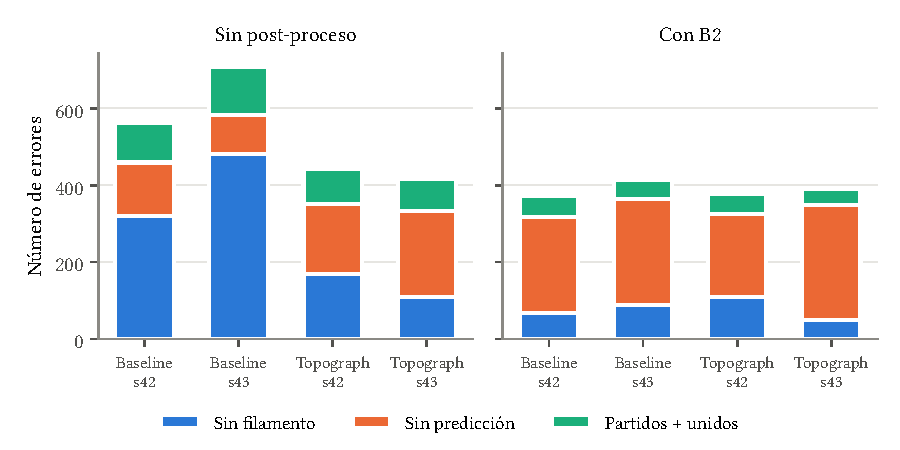
\includegraphics[width=\linewidth]{figuras/fig_tipos_error.pdf}
\caption{Tipos de error en val~$B$ de la baseline y de Topograph, con las
dos semillas, sin post-proceso (izquierda) y con B2 (derecha). Las
predicciones sin filamento y los filamentos sin predicción son errores
de presencia; los partidos y unidos, de estructura. Los valores están
en la Tabla~\ref{tab:res-asignaciones}.}
\label{fig:tipos-error}
\end{figure}

Esto aconseja también no quedarse solo con el PQ. La métrica resume en
un número errores de naturaleza muy distinta, y penaliza de forma
parecida no detectar un filamento, predecir uno donde no lo hay o partir
uno en dos. Por eso el resto del capítulo mira, además del PQ, qué
errores comete cada método, y usa B2 como post-proceso de referencia.

% ------------------------------------------------------------
\section{La topología en el entrenamiento}
\label{sec:res-perdidas}
% ------------------------------------------------------------

Para estudiar el efecto de las pérdidas topológicas se compararon diez
combinaciones de BCE con Dice, IoU y clDice, cada una con y sin
Topograph (Tabla~\ref{tab:perdidas}). Una de las pérdidas falla por
completo, con y sin Topograph. clDice sin Dice no llega a entrenar, porque compara
esqueletos pero no controla la extensión de la máscara
(Sección~\ref{sec:dice-cldice}), y se deja fuera del análisis.

\subsection{Predicciones más fiables}

El efecto más claro de Topograph no está en cuántos filamentos encuentra,
sino en la fiabilidad de lo que predice. Sin post-proceso, todas las
variantes con Topograph son más precisas que todas las variantes sin él,
y los dos grupos quedan separados en la Figura~\ref{fig:prec-exh}
(izquierda). La diferencia procede de las predicciones sin filamento,
que se reducen entre un 38 y un 63\,\% al añadir Topograph a
cualquiera de las pérdidas; con Dice, por ejemplo, pasan de 319 a 169. El precio es
una exhaustividad algo menor, porque el modelo deja de predecir algunos
filamentos dudosos.

\begin{figure}[ht]
\centering
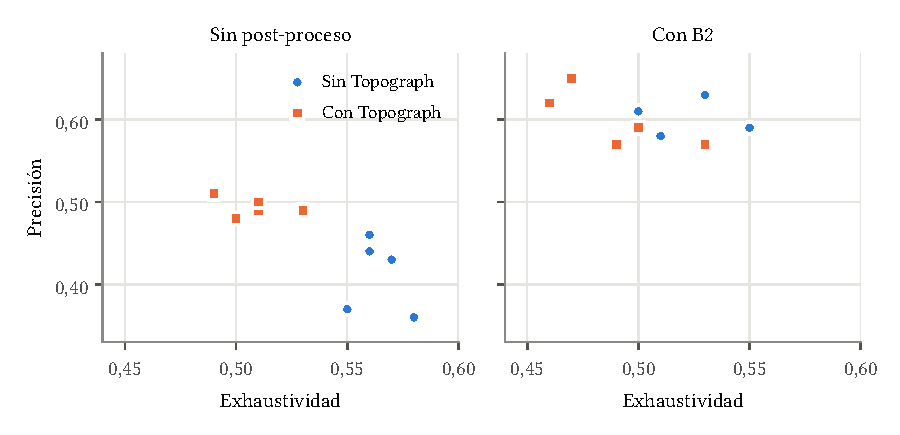
\includegraphics[width=\linewidth]{figuras/fig_precision_exhaustividad.pdf}
\caption{Precisión frente a exhaustividad en val~$B$, sin post-proceso
(izquierda) y con B2 (derecha). Cada punto es un modelo (las ocho
pérdidas, con las dos semillas de la baseline y de Topograph); en
naranja, las variantes con Topograph. Los valores están en
la Tabla~\ref{tab:res-fiabilidad}.}
\label{fig:prec-exh}
\end{figure}

Este comportamiento es el que cabe esperar de cómo actúa la pérdida
(Sección~\ref{sec:topograph}). Una componente predicha que no
corresponde a ningún filamento es una región crítica, un error que
cambia el número de componentes, y Topograph la penaliza. El modelo
aprende así a no predecir una componente salvo que esté bien respaldada
por la imagen. En este problema, en el que dos expertos solo coinciden
en un PQ de aproximadamente $0{,}34$ (Sección~\ref{sec:techo-humano}),
un modelo cuyas detecciones son casi siempre filamentos reales tiene un
valor que el PQ no recoge del todo.

Aun así, la mejora llega también al PQ. Sin post-proceso, Topograph es
la pérdida con mejor resultado, en val~$A$ y en val~$B$, y la única cuya
ventaja sobre la baseline se repite en tres entrenamientos
independientes. Las demás variantes topológicas también superan a la
baseline, mientras que IoU, sin sesgo topológico, queda por debajo. La
estructura mejora en la misma dirección, ya que añadir clDice o Topograph
reduce siempre los filamentos partidos, y las fusiones son poco
frecuentes en todos los modelos.

\subsection{Topograph y el filtro de área}
\label{sec:res-topograph}

La pregunta natural es qué ocurre cuando, además, se aplica el filtro de
área, que también elimina predicciones sin filamento y lo hace con
cualquier modelo. Con B2, la precisión de todos los modelos sube y los
dos grupos de la Figura~\ref{fig:prec-exh} (derecha) se mezclan. La
Tabla~\ref{tab:res-topo} y el panel derecho de la
Figura~\ref{fig:tipos-error} muestran qué queda entonces de la
diferencia entre la baseline y Topograph.

\begin{table}[ht]
\centering
\small
\begin{tabular}{@{}llccccc@{}}
\toprule
Pérdida & Post & PQ & P.\,+\,U. & Sin fil. & FP & Prec.\\
\midrule
Baseline (s42)  & sin & 0,311 & 104 & 319 & 665 & 0,43\\
Topograph (s42) & sin & 0,327 & 91  & 169 & 481 & 0,49\\
Baseline (s43)  & sin & 0,287 & 125 & 482 & 899 & 0,36\\
Topograph (s43) & sin & 0,322 & 81  & 110 & 402 & 0,51\\
\midrule
Baseline (s42)  & B2 & \textbf{0,373} & 55 & 68  & 269 & 0,63\\
Topograph (s42) & B2 & 0,354 & 53 & 108 & 342 & 0,57\\
Baseline (s43)  & B2 & 0,357 & 50 & 88  & 279 & 0,61\\
Topograph (s43) & B2 & 0,355 & \textbf{40} & \textbf{49} & \textbf{220} & \textbf{0,65}\\
\bottomrule
\end{tabular}
\caption{Baseline y Topograph en val~$B$, con las dos semillas, sin
post-proceso y con B2. P.\,+\,U.: filamentos partidos más unidos
(errores de estructura). Sin fil.: predicciones que no tocan ningún
filamento. FP: falsos positivos de la métrica oficial. Prec.:
precisión. En negrita, el mejor valor de cada columna. Las diez pérdidas
están en las Tablas~\ref{tab:res-asignaciones}
y~\ref{tab:res-fiabilidad}.}
\label{tab:res-topo}
\end{table}

Con la semilla 43, Topograph con B2 es el modelo que menos filamentos
parte o une, el que menos predicciones sin filamento y menos falsos
positivos comete, y el de mayor precisión de toda la comparación de
pérdidas. Sus predicciones son, por tanto, las que con más frecuencia
corresponden a un filamento real, algo que, de nuevo, tiene valor dado
el desacuerdo entre los propios expertos.

Esta ventaja, sin embargo, no aparece en el PQ, y la lectura topológica
ayuda a entender por qué. Una predicción sin filamento es una componente
de $H_0$ sin correspondencia en la referencia. Topograph enseña al
modelo a no crearla, y el filtro de área la elimina después por su
tamaño, así que los dos actúan sobre la misma clase de error. El filtro
mejora también mucho a la baseline, y las diferencias de PQ entre ambas
quedan dentro del ruido. Lo que queda de ventaja de Topograph se ve en
la estructura y en la fiabilidad de las predicciones, más que en la
métrica.

Conviene matizar que esta ventaja con B2 es clara con una semilla y
mucho menor con la otra. Con la semilla 42, Topograph solo mejora
ligeramente a la baseline en partidos y unidos, y no en predicciones sin
filamento ni en precisión. Sin post-proceso, en cambio, la mejora en
fiabilidad se repite con las dos semillas.

La semilla fija la inicialización de la red y el orden en que se le
presentan los datos durante el entrenamiento. Con todo lo demás igual,
pasar de la semilla 42 a la 43 cambia la comparación entre Topograph y
la baseline con B2, así que hay que ser prudente con las diferencias que
salen de una sola ejecución. Para medir la incertidumbre
de cada comparación se usa un \emph{bootstrap} pareado por días
(Capítulo~\ref{cap:metodologia}). Este método simula qué habría pasado
si val~$B$ estuviera formada por otros días. Una diferencia entre dos
modelos se considera significativa si su intervalo del 95\,\% no
contiene el $0$, es decir, si en casi todos los remuestreos uno de los
dos modelos queda por encima del otro. Pero
los modelos que compara son siempre los mismos, ya entrenados, así que
no tiene en cuenta que, al volver a entrenarlos, saldrían algo
distintos. Esto se ve al comparar la baseline consigo misma. Las
semillas 42 y 43 corresponden a la misma configuración, y aun así el
\emph{bootstrap} da la de la semilla 43 como significativamente peor,
con $0{,}024$ menos de PQ sin post-proceso
(Sección~\ref{sec:res-bootstrap}). Una diferencia «significativa» puede
deberse, por tanto, a que una ejecución salió especialmente bien o mal,
y por eso el trabajo se fija sobre todo en lo que se repite entre
semillas. Topograph mejora a la baseline sin post-proceso con ambas, lo
que apunta a una mejora real. Con B2, en cambio, las diferencias son del
mismo orden que la que separa a las dos semillas de la baseline.

Queda un último aspecto de la Figura~\ref{fig:tipos-error}, visible al
comparar sus dos paneles. El filtro de
área no es gratuito, porque elimina también filamentos reales pequeños,
y con B2 los filamentos sin predicción pasan a ser el error principal en
todos los modelos. Esto abre la pregunta de la siguiente sección, la de si un
criterio topológico, en lugar del tamaño, podría eliminar las
componentes espurias sin perder esos filamentos.

% ------------------------------------------------------------
\section{La topología en el post-proceso}
\label{sec:res-e2}
% ------------------------------------------------------------

La lectura topológica sugiere sustituir el tamaño por la robustez, es
decir, conservar las componentes con persistencia alta en el diagrama
$H_0$ aunque sean pequeñas. Si los filamentos pequeños son robustos y
las predicciones espurias no, un filtro así eliminaría las segundas sin
perder los primeros. Se probaron dos variantes
(Sección~\ref{sec:postproceso}). E2 sustituye el área por la
persistencia y une las componentes separadas por un collado cercano al
umbral, y B2+P conserva una componente si es grande \emph{o} si es
robusta. La Tabla~\ref{tab:res-e2-resumen} las compara en dos modelos
representativos, y la Sección~\ref{sec:anx-e2} recoge los once modelos
en los que se probaron. En PQ las diferencias son pequeñas, así que la
comparación se centra en qué errores corrige cada una.

\begin{table}[ht]
\centering
\small
\begin{tabular}{@{}llccccc@{}}
\toprule
Modelo & Post & PQ & P.\,+\,U. & Sin pred. & Sin fil. & Prec.\\
\midrule
Baseline & sin  & 0,303 & 112 & 143 & 318 & 0,41\\
         & B2   & \textbf{0,368} & 49  & 255 & 72  & 0,63\\
         & E2   & 0,314 & 91  & 142 & 279 & 0,44\\
         & B2+P & \textbf{0,368} & 36  & 213 & 116 & 0,60\\
\midrule
Topograph & sin  & 0,330 & 88  & 189 & 158 & 0,50\\
          & B2   & \textbf{0,362} & 52  & 237 & 89  & 0,61\\
          & E2   & 0,339 & 76  & 191 & 139 & 0,52\\
          & B2+P & \textbf{0,362} & \textbf{34} & 235 & 93 & 0,61\\
\bottomrule
\end{tabular}
\caption{Post-procesos en val~$B$ sobre el mejor intento del ajuste de
hiperparámetros de la baseline y de Topograph. En negrita, el mejor PQ
de cada modelo y el menor número de partidos y unidos. P.\,+\,U.: filamentos
partidos más unidos (errores de estructura). Sin pred.\ y Sin fil.:
errores de presencia. Prec.: precisión. Los once modelos están en las
Tablas~\ref{tab:res-e2} y~\ref{tab:res-e2-errores}.}
\label{tab:res-e2-resumen}
\end{table}

E2 hace lo que se esperaba de un filtro que decide por robustez y no por
tamaño. No pierde filamentos, porque los que quedan sin predicción son
prácticamente los mismos que sin post-proceso, mientras que B2 pierde
muchos. De hecho, la baseline de referencia con E2 tiene la mayor
exhaustividad de todas las combinaciones probadas, $0{,}595$, incluso
ligeramente por encima de la predicción sin post-proceso
(Tabla~\ref{tab:res-e2-errores}). Además, reduce los filamentos partidos por dos vías. La fusión
por collado une trozos separados por un hueco pequeño, y el filtro
elimina trozos poco persistentes, como el máximo $B$ del
Ejemplo~\ref{ej:perfil}.

Su debilidad está en las predicciones espurias. Con la baseline, E2
apenas las reduce, y el ajuste elige un umbral de persistencia casi
nulo, porque uno mayor eliminaría también muchos aciertos. La razón es
que la baseline está muy segura incluso cuando se equivoca. Una mancha
aislada con un pico de probabilidad de $0{,}9$ sobre un fondo cercano a
0 tiene una persistencia $b-d\approx0{,}9$, tan alta como la de un
filamento real, de modo que en un modelo así la persistencia se reduce
prácticamente a la confianza del pico. El diagnóstico de la
Sección~\ref{sec:diagnostico} ya mostraba que las espurias tienen casi
la misma confianza que los aciertos. Lo que las distingue es su tamaño,
y eso es justo lo que la persistencia de $H_0$ no tiene en cuenta. Con
Topograph, cuyas espurias son menos robustas, E2 elimina bastantes más,
y sus errores de presencia llegan a ser del mismo orden que los de B2,
aunque repartidos de otra forma, con menos filamentos perdidos y más
espurias.

Combinar ambos criterios resuelve en parte el problema. B2+P filtra por
tamaño de forma más estricta que B2 y rescata solo las componentes
pequeñas casi seguras, así que la persistencia actúa aquí como un
criterio de confianza. En los dos modelos de la tabla iguala el PQ de B2 y deja muy pocos
errores de estructura. Aplicado a los once modelos
(Sección~\ref{sec:anx-e2}), el resultado depende de Topograph. En los
cinco modelos entrenados con él, B2+P iguala o mejora ligeramente el PQ
de B2, con menos errores de estructura y mayor precisión. En los seis
entrenados sin él, el PQ queda igual o por debajo y la precisión baja
siempre, porque la persistencia rescata también espurias muy seguras.
Parte de esa diferencia puede deberse al ajuste, que en cinco de esos
seis modelos no llega a igualar a B2 en val~$A$ aunque podría hacerlo.
La combinación de Topograph y B2+P es, por tanto, la más favorable del
trabajo desde el punto de vista topológico, con la cautela de que la
baseline queda cerca y de que todo procede de un único entrenamiento por
modelo.

% ------------------------------------------------------------
\section{Alcance de los resultados}
\label{sec:res-alcance}
% ------------------------------------------------------------

\subsection{Barbas}
\label{sec:res-barbas}

Las barbas, que motivaron el uso de clDice, son la parte del filamento
que peor se recupera, y ninguna pérdida topológica mejora su detección.
Los modelos cubren la mayor parte de la espina, pero solo alrededor de la
mitad de las barbas. El problema no está en la resolución de salida,
porque la anotación reducida a $512\times512$ conserva casi todas las
barbas, y los post-procesos por persistencia tampoco cambian su
detección. clDice, en concreto, la empeora en todas las combinaciones, porque hace que el modelo prediga más estructura
alrededor del filamento pero no más barbas reales. Los detalles están en
la Sección~\ref{sec:anx-barbas}.

\subsection{Ajuste de hiperparámetros}
\label{sec:res-hp}

La comparación de pérdidas usa una configuración común, que podría
favorecer a algún modelo. Para comprobarlo se ajustaron los
hiperparámetros de la baseline, Topograph y clDice
(Sección~\ref{sec:anx-hp}). El ajuste mejora algo a las dos pérdidas
topológicas y no a la baseline, pero tras él los tres modelos quedan
dentro del ruido, así que la comparación no cambia.

\subsection{Test de la competición}
\label{sec:res-test}

En el \emph{leaderboard} público de la competición, todos los modelos
enviados obtienen un PQ entre $0{,}26$ y $0{,}30$, entre $0{,}06$ y
$0{,}10$ por debajo de val~$B$. La caída es parecida en todas las
configuraciones y el orden entre ellas se mantiene, con B2+P igual o
algo por encima de B2 y E2 por debajo. La distribución de estaciones y de años es parecida en
entrenamiento y test, así que no parece explicarla, y no es posible
estudiarla más a fondo porque las anotaciones del test no son públicas. Con un solo envío por
configuración y la mitad del test, las diferencias entre envíos no son
concluyentes (Sección~\ref{sec:anx-test}).

% ============================================================
% Capítulo 7 — Conclusiones
% ============================================================

\chapter{Conclusiones}
\label{cap:conclusiones}

% ------------------------------------------------------------
\section{Conclusiones}
% ------------------------------------------------------------

\paragraph{Fundamentos (O1).} La homología persistente da un lenguaje
preciso para los errores que más pesan en la segmentación de
estructuras finas. Un filamento partido, dos filamentos fusionados o una
componente espuria son cambios en el número de Betti $\beta_0$, y su
robustez frente al umbral se lee en el diagrama de persistencia.
Topograph traduce esa idea en una pérdida que actúa solo sobre las
regiones críticas, con un coste casi lineal.

\paragraph{Protocolo (O2).} Todas las decisiones se toman en una mitad
de la validación y la cifra se reporta en la otra, con la métrica
oficial y una partición por días. Esta separación ha resultado
necesaria: la variación entre semillas, de hasta $0{,}024$ en PQ, es del
mismo orden que las diferencias entre pérdidas, y el \emph{bootstrap}
por días no la recoge. Sin esta precaución, varias de las comparaciones
habrían parecido concluyentes.

\paragraph{Diagnóstico (O3).} Leído sobre el diagrama $H_0$, el
post-proceso clásico es un filtro sobre las componentes del conjunto de
supernivel que solo mira su tamaño. Su efecto es grande: el área mínima
sube el PQ de la baseline de $0{,}311$ a $0{,}373$, porque la mayoría de
los falsos positivos son componentes pequeñas. El umbral, por sí solo,
no aporta nada.

\paragraph{Pérdidas topológicas (O4).} Sin post-proceso, Topograph
mejora a la baseline con las dos semillas probadas, y es la única pérdida
con una mejora significativa. clDice reduce la fragmentación, coherente
con que premia la continuidad. Pero la mejora de Topograph viene sobre
todo de eliminar componentes espurias, que es lo mismo que hace el
filtro de área. Con el post-proceso ajustado, ninguna pérdida supera a
la baseline. La conclusión es que, en este problema, el sesgo
topológico introducido en el entrenamiento y el filtro clásico aplicado
después corrigen el mismo tipo de error, y sus mejoras no se suman.
El resultado se repite en tres entrenamientos independientes y resiste
el ajuste de hiperparámetros: ajustadas, Topograph y clDice se acercan
a la baseline, pero no la superan.

En cuanto a las barbas, la hipótesis de partida no se cumple. Son la
parte del filamento que peor se recupera, aunque la anotación reducida a
la resolución de trabajo las conserva casi enteras, y ninguna pérdida
topológica las mejora. clDice, que se eligió precisamente por ellas,
hace que el modelo prediga más estructura junto al filamento pero no
más barbas reales: su precisión baja en todas las combinaciones
probadas. Las barbas pesan muy poco en el esqueleto total, y una
pérdida que premia la continuidad del esqueleto acaba optimizando la
de la espina.

% ------------------------------------------------------------
\section{Limitaciones}
% ------------------------------------------------------------

\begin{itemize}
  \item \emph{Una ejecución por pérdida.} Solo la baseline y Topograph
  se han entrenado con dos semillas. Dada la variación observada entre
  semillas, las diferencias pequeñas entre pérdidas no pueden
  confirmarse.
  \item \emph{Resolución.} El modelo trabaja a $512\times512$, un cuarto
  de la resolución original en cada eje. Para las barbas esto apenas
  importa (la anotación reducida conserva el 99,7\,\% de su esqueleto),
  pero limita la precisión con que se delimita el contorno.
  \item \emph{Ajuste limitado.} La comparación completa de pérdidas usa
  una configuración común, sin aumentos de datos. El ajuste de la
  Sección~\ref{sec:res-hp} muestra que esa configuración favorecía algo
  a la baseline, pero solo cubre tres modelos y 3 horas por modelo.
  \item \emph{Una sola arquitectura}, la U-Net con ResNet-34.
\end{itemize}

% ------------------------------------------------------------
\section{Trabajo futuro}
% ------------------------------------------------------------

\begin{itemize}
  \item \textbf{Post-proceso por persistencia (E2).} Es la continuación
  más directa. Si Topograph y el filtro de área corrigen el mismo error,
  un filtro que decida sobre la persistencia de cada componente, y no
  sobre su área, podría conservar los filamentos pequeños pero robustos
  que el filtro de área elimina. La fusión por proximidad del collado
  atacaría además los fragmentados recuperables, que ningún método
  probado corrige.
  \item \textbf{Estrategias de etiquetas (E4).} Comparar el
  entrenamiento con cada anotación por separado con la media de las
  anotaciones y con los filamentos de la mayoría.
  \item \textbf{Más semillas por pérdida}, para separar las diferencias
  reales del ruido del entrenamiento.
  \item \textbf{Pérdidas centradas en las barbas.} Como la resolución
  no es el límite, mejorar las barbas pasa por cambiar lo que aprende
  la red, por ejemplo dando más peso a la zona de barbas en la pérdida.
  \item \textbf{Otras pérdidas topológicas}, como Betti
  matching~\cite{stucki2023}, que garantiza la correspondencia espacial
  de las estructuras a mayor coste computacional.
\end{itemize}


\appendix
% ============================================================
% Apéndice A — Código y reproducibilidad
% ============================================================

\chapter{Código y reproducibilidad}
\label{ap:codigo}

Todo el código del trabajo es público en
\url{https://github.com/AgustinG-git/tfm-filamentos}. La versión que
corresponde a esta memoria está marcada con la etiqueta
\texttt{v1.0-deposito}. Este apéndice describe cómo está organizado y
cómo se reproduce cada resultado.

% ------------------------------------------------------------
\section{Organización}
% ------------------------------------------------------------

El código se divide en una biblioteca, \texttt{filseg}, con las piezas
del protocolo, y una serie de \emph{scripts} que las combinan para cada
experimento (Tablas~\ref{tab:modulos} y~\ref{tab:scripts}). Las
configuraciones de cada experimento son ficheros YAML en
\texttt{configs/}, que heredan de la baseline y cambian solo la pieza que
se estudia.

\begin{table}[ht]
\centering
\small
\begin{tabular}{@{}lp{10.5cm}@{}}
\toprule
Módulo & Contenido\\
\midrule
\texttt{contract.py} & Decisiones congeladas comunes a todas las ejecuciones (partición, resoluciones, criterio de selección, ficheros de salida). No se modifica.\\
\texttt{split.py} & Partición entrenamiento / val~$A$ / val~$B$ agrupada por fecha, generada una sola vez.\\
\texttt{gt.py} & Referencia de evaluación en el formato oficial, a partir del JSON de MAGFiLO.\\
\texttt{data.py} & Carga de imágenes a $512\times512$ y etiquetas de entrenamiento.\\
\texttt{model.py} & U-Net con codificador ResNet-34~\cite{iakubovskii2019}.\\
\texttt{losses.py} & Las pérdidas de la Tabla~\ref{tab:perdidas}: BCE, Dice, IoU, clDice y Topograph, con su calentamiento.\\
\texttt{train.py} & Una ejecución completa: entrenamiento, selección de la época en val~$A$, evaluación y registro.\\
\texttt{postproc.py} & Post-procesos: umbral y componentes conexas con filtro de área (B1, B2) filtro por persistencia (E2) y su combinación con el área (B2+P).\\
\texttt{postrun.py} & Ajuste en val~$A$ de un post-proceso sobre una ejecución ya entrenada, sin reentrenar.\\
\texttt{official\_metric.py} & Copia literal del cuaderno oficial de autoevaluación de la competición~\cite{kaggle2026}.\\
\texttt{metrics.py} & Evaluación con la métrica oficial y comprobaciones previas (formato, solapes).\\
\texttt{compare.py} & Conteos por anotación, relaciones 1:$n$ y $n$:1 y \emph{bootstrap} pareado por días.\\
\texttt{runs.py} & Identificadores, salidas de cada ejecución y tabla de registro.\\
\bottomrule
\end{tabular}
\caption{Módulos de la biblioteca \texttt{filseg}.}
\label{tab:modulos}
\end{table}

\begin{table}[ht]
\centering
\small
\begin{tabular}{@{}lp{10.5cm}@{}}
\toprule
\emph{Script} & Uso\\
\midrule
\texttt{make\_split.py} & Genera la partición (una sola vez).\\
\texttt{entrenar.py} & Lanza una ejecución a partir de una configuración.\\
\texttt{cola.sh} & Encadena varias ejecuciones en la misma GPU.\\
\texttt{postproceso.py} & Aplica B1 y B2 a las ejecuciones entrenadas (Sección~\ref{sec:res-post}).\\
\texttt{e2.py} & Aplica los post-procesos por persistencia (E2 y B2+P).\\
\texttt{ajuste\_hp.py} & Ajuste de hiperparámetros con Optuna (Sección~\ref{sec:res-hp}).\\
\texttt{resultados.py} & \emph{Bootstrap} y relaciones del Capítulo~\ref{cap:resultados}.\\
\texttt{barbas.py} & Medida de barbas y techo a $512\times512$ (Sección~\ref{sec:res-barbas}).\\
\texttt{medir\_topograph.py} & Escala del término de Topograph, para fijar $\alpha$.\\
\texttt{figura\_magfilo.py} & Figura~\ref{fig:magfilo}.\\
\bottomrule
\end{tabular}
\caption{\emph{Scripts} de los experimentos.}
\label{tab:scripts}
\end{table}

Topograph se usa a través de la implementación oficial de sus
autores~\cite{lux2025}, con su extensión compilada en C++. El
repositorio incluye además pruebas automáticas (\texttt{tests/}) que
comprueban, entre otras cosas, que la evaluación propia coincide con la
oficial y que la partición no comparte días entre subconjuntos.

% ------------------------------------------------------------
\section{Reproducir un resultado}
% ------------------------------------------------------------

Cada ejecución lee los datos de la carpeta indicada en
\texttt{FILSEG\_DATA} y escribe en \texttt{FILSEG\_OUT}. Por ejemplo, la
baseline y su post-proceso B2:

\begin{verbatim}
python scripts/entrenar.py configs/base.yaml
python scripts/postproceso.py --filtro "_base_"
\end{verbatim}

Cada ejecución crea una carpeta \texttt{runs/<run\_id>}, donde el
identificador combina la fecha, la configuración y el \emph{commit} del
código, con la configuración completa, la época elegida, las
predicciones y los \emph{logits} de validación y el envío para la
competición. Además añade una fila a \texttt{registro.csv} con sus
métricas en val~$A$ y val~$B$, y sus conteos a \texttt{conteos.csv}. Las
tablas del Capítulo~\ref{cap:resultados} salen de esos dos ficheros, que
están en el repositorio. Como el entrenamiento en GPU no es determinista,
repetir una ejecución reproduce sus cifras con una diferencia del orden
de $0{,}01$--$0{,}02$ en PQ (Sección~\ref{sec:evaluacion}).

% ------------------------------------------------------------
\section{Post-proceso por persistencia}
% ------------------------------------------------------------

Como ejemplo de cómo se traduce la teoría del
Capítulo~\ref{cap:fundamentos} a código, este es el núcleo del
post-proceso por persistencia (comentarios simplificados). Con
\texttt{area\_min} se obtiene la variante B2+P; sin él, E2. El filtro por persistencia
se apoya en los $h$-máximos: los máximos regionales de altura al menos
$\tau$ son exactamente los puntos del diagrama $H_0$ de superniveles con
persistencia $b-d\ge\tau$. Se ha comprobado, sobre imágenes sintéticas,
que la selección coincide con la que se obtiene calculando el diagrama
con \emph{union-find} y la regla del mayor
(Sección~\ref{sec:persistencia-eficiente}).

\begin{small}
\begin{verbatim}
def persistencia_512(prob, umbral, tau, delta, area_min=None):
    # X_t = {prob > umbral}, componentes 8-conexas
    xt = (prob > umbral).astype(np.uint8)
    n_t, lt = cv2.connectedComponents(xt, connectivity=8)
    # h-maximos: maximos con persistencia b - d >= tau
    hmax = h_maxima(prob, tau, footprint=np.ones((3, 3))) > 0
    keep = np.unique(lt[hmax & (xt > 0)])
    if area_min is not None:     # B2+P: area O persistencia
        areas = np.bincount(lt.ravel())
        keep = np.union1d(keep, np.flatnonzero(areas >= area_min))
    vivo = np.isin(lt, keep[keep > 0])
    # fusion por collado: unidas en X_{t - delta} -> una instancia
    _, ld = cv2.connectedComponents(
        (prob > umbral - delta).astype(np.uint8), connectivity=8)
    lab = np.where(vivo, ld, 0)
    return relabel(lab)          # etiquetas 1..n consecutivas
\end{verbatim}
\end{small}

% ============================================================
% Apéndice B — Resultados complementarios
% ============================================================

\chapter{Resultados complementarios}
\label{ap:resultados}

Este apéndice recoge las tablas completas de los experimentos del
Capítulo~\ref{cap:resultados}, con todas las pérdidas, post-procesos y
medidas. Todas las cifras son de val~$B$ salvo que se indique lo
contrario.

% ------------------------------------------------------------
\section{Post-proceso clásico}
\label{sec:anx-post}
% ------------------------------------------------------------

La Tabla~\ref{tab:anx-post} compara la búsqueda en rejilla y con Optuna
de los dos post-procesos clásicos sobre la baseline (semilla 42). Ambas
búsquedas llegan a valores parecidos, lo que indica que la rejilla ya
cubría la zona de buenos valores; en el trabajo se usa Optuna. Al subir
el umbral sin filtro de área, los falsos positivos aumentan
ligeramente, posiblemente porque algunas componentes se dividen.

\begin{table}[htbp]
\centering
\small
\begin{tabular}{@{}lccccccc@{}}
\toprule
Post-proceso & $t$ & $a$ & PQ & SQ & RQ & TP & FP / FN\\
\midrule
Sin post-proceso & 0,50 & 0 & 0,311 & 0,638 & 0,488 & 495 & 665 / 374\\
B1 (rejilla) & 0,65 & 0 & 0,314 & 0,647 & 0,485 & 494 & 674 / 375\\
B1 (Optuna) & 0,66 & 0 & 0,313 & 0,646 & 0,484 & 494 & 678 / 375\\
B2 (rejilla) & 0,65 & 25 & \textbf{0,375} & 0,649 & 0,577 & 473 & 297 / 396\\
B2 (Optuna) & 0,66 & 29 & 0,373 & 0,650 & 0,574 & 458 & 269 / 411\\
\bottomrule
\end{tabular}
\caption{Post-proceso de la baseline (semilla 42) en val~$B$. $t$ es el
umbral y $a$ el área mínima en píxeles a $512\times512$, ambos ajustados
en val~$A$.}
\label{tab:anx-post}
\end{table}

% ------------------------------------------------------------
\section{Comparación de pérdidas}
\label{sec:anx-perdidas}
% ------------------------------------------------------------

La Tabla~\ref{tab:res-perdidas} da el PQ de las diez pérdidas, en val~$A$
y val~$B$, sin post-proceso y con B2. La combinación de BCE y clDice sin
Dice colapsa. El mejor modelo en $A$ es el de la primera época (la sexta
con Topograph) y su PQ no llega a $0{,}05$ ni con post-proceso. Las
Tablas~\ref{tab:res-asignaciones} y~\ref{tab:res-fiabilidad} dan los
tipos de error y la fiabilidad de las detecciones. De ellas salen las
Figuras~\ref{fig:prec-exh} y~\ref{fig:tipos-error}.

Dos observaciones complementan las del capítulo. En partidos y unidos,
clDice es tan eficaz como Topograph, lo que concuerda con que premia la
continuidad de las estructuras alargadas, mientras que IoU, sin sesgo
topológico, llega a 123 filamentos partidos. Con B2, los filamentos
sin predicción suben en todos los modelos, hasta 201--301, y
IoU+Topograph es, tras Topograph (s43), el modelo con menos predicciones
sin filamento (54).

\begin{table}[htbp]
\centering
\small
\begin{tabular}{@{}lccccc@{}}
\toprule
 & & \multicolumn{2}{c}{Sin post-proceso} & \multicolumn{2}{c}{B2 (Optuna)}\\
\cmidrule(lr){3-4}\cmidrule(lr){5-6}
Pérdida & Época & PQ $A$ & PQ $B$ & PQ $A$ & PQ $B$\\
\midrule
Baseline (s42) & 8 & 0,297 & 0,311 & \textbf{0,364} & \textbf{0,373}\\
Baseline (s43) & 8 & 0,276 & 0,287 & 0,348 & 0,357\\
IoU & 15 & 0,279 & 0,285 & 0,351 & 0,351\\
clDice & 13 & 0,307 & 0,313 & 0,351 & 0,354\\
IoU+clDice & 14 & 0,308 & 0,322 & 0,345 & 0,363\\
clDice sin Dice & 1 & 0,012 & 0,009 & 0,062 & 0,036\\
\midrule
Topograph (s42) & 17 & \textbf{0,322} & \textbf{0,327} & 0,354 & 0,354\\
Topograph (s43) & 12 & 0,298 & 0,322 & 0,336 & 0,355\\
IoU+Topo & 16 & 0,315 & 0,315 & 0,346 & 0,346\\
clDice+Topo & 18 & 0,307 & 0,317 & 0,344 & 0,348\\
IoU+clDice+Topo & 18 & 0,297 & 0,318 & 0,333 & 0,336\\
clDice sin Dice+Topo & 6 & 0,025 & 0,014 & 0,080 & 0,045\\
\bottomrule
\end{tabular}
\caption{PQ de cada pérdida en val~$A$ y val~$B$, sin post-proceso
(umbral $0{,}5$, sin filtro de área) y con B2 ajustado en val~$A$ para
cada ejecución. La «Época» es la elegida en val~$A$ y la semilla se fija en 42 salvo que
se indique.}
\label{tab:res-perdidas}
\end{table}

\begin{table}[htbp]
\centering
\small
\begin{tabular}{@{}lcccccc@{}}
\toprule
Pérdida & Partidos & Unidos & P.\,+\,U. & Sin pred. & Sin fil. & S.\,P.\,+\,S.\,F.\\
\midrule
\multicolumn{7}{l}{\emph{Sin post-proceso}}\\
Baseline (s42) & 92 & \textbf{12} & 104 & 140 & 319 & 459\\
Baseline (s43) & 111 & 14 & 125 & \textbf{100} & 482 & 582\\
IoU & 123 & 13 & 136 & 119 & 380 & 499\\
clDice & 73 & 17 & 90 & 122 & 278 & 400\\
IoU+clDice & \textbf{57} & 15 & \textbf{72} & 124 & 261 & 385\\
Topograph (s42) & 78 & 13 & 91 & 183 & 169 & 352\\
Topograph (s43) & 68 & 13 & 81 & 224 & \textbf{110} & \textbf{334}\\
IoU+Topo & 79 & 13 & 92 & 199 & 142 & 341\\
clDice+Topo & 65 & 15 & 80 & 180 & 159 & 339\\
IoU+clDice+Topo & 63 & 18 & 81 & 197 & 161 & 358\\
\midrule
\multicolumn{7}{l}{\emph{B2 (Optuna)}}\\
Baseline (s42) & 43 & \textbf{12} & 55 & 250 & 68 & 318\\
Baseline (s43) & 37 & 13 & 50 & 275 & 88 & 363\\
IoU & 45 & 13 & 58 & 247 & 95 & 342\\
clDice & 39 & 15 & 54 & 213 & 119 & 332\\
IoU+clDice & 34 & 15 & 49 & \textbf{201} & 110 & \textbf{311}\\
Topograph (s42) & 41 & \textbf{12} & 53 & 217 & 108 & 325\\
Topograph (s43) & \textbf{26} & 14 & \textbf{40} & 300 & \textbf{49} & 349\\
IoU+Topo & 36 & 13 & 49 & 301 & 54 & 355\\
clDice+Topo & 37 & 14 & 51 & 240 & 82 & 322\\
IoU+clDice+Topo & 43 & 15 & 58 & 248 & 82 & 330\\
\bottomrule
\end{tabular}
\caption{Tipos de error en val~$B$, sumados sobre todos los pares
anotador--imagen. \emph{Partidos}: filamentos de referencia tocados por
dos o más predicciones. \emph{Unidos}: predicciones que tocan dos o más
filamentos. \emph{Sin pred.}: filamentos que ninguna predicción toca.
\emph{Sin fil.}: predicciones que no tocan ningún filamento. «Tocar»
significa solaparse en al menos un píxel ($\mathrm{IoU}>0$), como en la
definición oficial. P.\,+\,U.\ y S.\,P.\,+\,S.\,F.\ son las sumas que
miden los errores de estructura y de presencia
(Sección~\ref{sec:evaluacion}). En negrita, el menor valor de cada
columna dentro de cada bloque.}
\label{tab:res-asignaciones}

\end{table}

\begin{table}[htbp]
\centering
\small
\begin{tabular}{@{}lcccccc@{}}
\toprule
 & \multicolumn{3}{c}{Sin post-proceso} & \multicolumn{3}{c}{B2 (Optuna)}\\
\cmidrule(lr){2-4}\cmidrule(lr){5-7}
Pérdida & Prec. & Exh. & Sin fil.\ (\%) & Prec. & Exh. & Sin fil.\ (\%)\\
\midrule
Baseline (s42) & 0,43 & 0,57 & 27,5 & 0,63 & 0,53 & 9,4\\
Baseline (s43) & 0,36 & 0,58 & 34,4 & 0,61 & 0,50 & 12,4\\
IoU & 0,37 & 0,55 & 29,3 & 0,58 & 0,51 & 12,5\\
clDice & 0,44 & 0,56 & 25,2 & 0,57 & 0,53 & 14,7\\
IoU+clDice & 0,46 & 0,56 & 24,6 & 0,59 & 0,55 & 13,7\\
\midrule
Topograph (s42) & \textbf{0,49} & 0,53 & \textbf{18,0} & 0,57 & 0,53 & 13,5\\
Topograph (s43) & \textbf{0,51} & 0,49 & \textbf{13,4} & \textbf{0,65} & 0,47 & \textbf{7,8}\\
IoU+Topo & \textbf{0,48} & 0,50 & \textbf{15,8} & 0,62 & 0,46 & \textbf{8,3}\\
clDice+Topo & \textbf{0,49} & 0,51 & \textbf{17,4} & 0,59 & 0,50 & 11,1\\
IoU+clDice+Topo & \textbf{0,50} & 0,51 & \textbf{18,2} & 0,57 & 0,49 & 11,2\\
\bottomrule
\end{tabular}
\caption{Fiabilidad de las detecciones en val~$B$. Prec.: aciertos entre
predicciones, $\mathrm{TP}/(\mathrm{TP}+\mathrm{FP})$. Exh.: aciertos
entre filamentos de referencia, $\mathrm{TP}/869$. Sin fil.: porcentaje
de predicciones que no tocan ningún filamento. En negrita, los valores
en los que todas las variantes con Topograph mejoran a todas las
variantes sin él.}
\label{tab:res-fiabilidad}
\end{table}

% ------------------------------------------------------------
\section{Incertidumbre de las comparaciones}
\label{sec:res-bootstrap}
% ------------------------------------------------------------

La Tabla~\ref{tab:res-bootstrap} da la diferencia de PQ de cada
ejecución con la baseline (semilla 42) y su intervalo del 95\,\%,
obtenido por \emph{bootstrap} pareado por días
(Capítulo~\ref{cap:metodologia}). Sin post-proceso, solo Topograph con
la semilla 42 mejora a la baseline de forma significativa; con la
semilla 43 también la mejora ($+0{,}011$), pero su intervalo incluye el
0, e IoU es significativamente peor. Con B2, siete de las nueve
ejecuciones quedan significativamente por debajo.

Estos intervalos deben leerse con cuidado. La baseline con la semilla 43
es significativamente peor que con la 42 sin post-proceso
($-0{,}024$) y casi lo es con B2, a pesar de tratarse de la misma
configuración. El \emph{bootstrap} por días mide cuánto depende el PQ de
los días que forman val~$B$, pero no la variabilidad del propio
entrenamiento. Con una sola ejecución por pérdida, una diferencia
«significativa» puede deberse a que la ejecución de referencia salió
especialmente bien o mal.

\begin{table}[htbp]
\centering
\small
\begin{tabular}{@{}lcccc@{}}
\toprule
 & \multicolumn{2}{c}{Sin post-proceso} & \multicolumn{2}{c}{B2 (Optuna)}\\
\cmidrule(lr){2-3}\cmidrule(lr){4-5}
Pérdida & $\Delta$PQ & IC 95\,\% & $\Delta$PQ & IC 95\,\%\\
\midrule
Baseline (s42) & --- & --- & --- & --- \\
Baseline (s43) & $-0{,}024^*$ & $[-0{,}039,\,-0{,}009]$ & $-0{,}016$ & $[-0{,}035,\,+0{,}005]$ \\
IoU & $-0{,}026^*$ & $[-0{,}044,\,-0{,}010]$ & $-0{,}022^*$ & $[-0{,}037,\,-0{,}007]$ \\
clDice & $+0{,}002$ & $[-0{,}011,\,+0{,}016]$ & $-0{,}019^*$ & $[-0{,}036,\,-0{,}002]$ \\
IoU+clDice & $+0{,}011$ & $[-0{,}004,\,+0{,}024]$ & $-0{,}010$ & $[-0{,}030,\,+0{,}011]$ \\
Topograph (s42) & $+0{,}016^*$ & $[+0{,}001,\,+0{,}032]$ & $-0{,}020^*$ & $[-0{,}035,\,-0{,}001]$ \\
Topograph (s43) & $+0{,}011$ & $[-0{,}008,\,+0{,}029]$ & $-0{,}019^*$ & $[-0{,}035,\,-0{,}003]$ \\
IoU+Topo & $+0{,}004$ & $[-0{,}017,\,+0{,}025]$ & $-0{,}028^*$ & $[-0{,}047,\,-0{,}008]$ \\
clDice+Topo & $+0{,}005$ & $[-0{,}010,\,+0{,}022]$ & $-0{,}025^*$ & $[-0{,}044,\,-0{,}006]$ \\
IoU+clDice+Topo & $+0{,}007$ & $[-0{,}009,\,+0{,}022]$ & $-0{,}037^*$ & $[-0{,}055,\,-0{,}019]$ \\
\bottomrule
\end{tabular}
\caption{Diferencia de PQ en val~$B$ con la baseline (semilla 42) e
intervalo del 95\,\% (\emph{bootstrap} pareado por días, 2.000
remuestreos). $^*$: el intervalo no contiene el 0.}
\label{tab:res-bootstrap}
\end{table}

% ------------------------------------------------------------
\section{Post-proceso por persistencia}
\label{sec:anx-e2}
% ------------------------------------------------------------

E2 y B2+P se aplicaron a ejecuciones reentrenadas con la semilla 42, que son las
ocho pérdidas con la configuración común (\emph{ref.}) y los mejores
intentos del ajuste de hiperparámetros de la baseline, clDice y
Topograph (\emph{mejor}). Las ejecuciones de la Tabla~\ref{tab:res-perdidas}
no se conservaron, y por el no determinismo del entrenamiento las cifras
de los reentrenamientos difieren algo de las suyas. E2 se aplicó a los
once modelos y B2+P también (Tablas~\ref{tab:res-e2}
y~\ref{tab:res-b2p}). Los tipos de error de los cuatro post-procesos se
detallan para seis de ellos (Tabla~\ref{tab:res-e2-errores}).

\paragraph{E2.} Queda por debajo de B2 en PQ en los once modelos, entre
$0{,}03$ y $0{,}06$ sin Topograph y entre $0{,}004$ y $0{,}024$ con
Topograph. En cinco de los seis modelos de la
Tabla~\ref{tab:res-e2-errores}, los filamentos sin predicción quedan al
nivel de la predicción sin post-proceso (B2 los aumenta en entre 48 y
141) y E2 es, de los tres
post-procesos, el que conserva más espina; la excepción es clDice+Topo,
para el que el ajuste elige un umbral alto ($0{,}68$). El ajuste elige
$\delta$ entre $0{,}22$ y $0{,}30$ en nueve de los once modelos, y los
partidos bajan en los seis respecto a la predicción sin post-proceso,
con un coste en fusiones pequeño (los unidos suben como mucho en 7). Los partidos pasan
de 132 a 107 en la baseline de referencia y de 88 a 45 en Topograph de
referencia. En la baseline, donde $\tau$ es casi nulo y el filtro apenas
actúa, la reducción se debe a la fusión; con Topograph, el filtro
elimina además trozos poco persistentes. B2 deja aún menos partidos en
cinco de los seis modelos, pero lo consigue eliminando componentes
pequeñas, entre ellas fragmentos, y con ello también filamentos
enteros.
Para la baseline, el ajuste elige un $\tau$ casi nulo
($0{,}03$--$0{,}06$), y E2 elimina solo un 10--12\,\% de las
predicciones sin filamento; con Topograph elimina entre un 12 y un
38\,\%, frente a un 3--12\,\% en las ejecuciones sin él. Por eso, con la baseline, los errores de presencia
de E2 son muy superiores a los de B2 (421--479 frente a 321--327),
mientras que con Topograph son del mismo orden (321--342 frente a
320--345), aunque con otra composición: E2 pierde menos filamentos y
deja más espurias.

\paragraph{B2+P.} El resultado depende de si el modelo se entrenó con
Topograph (Tabla~\ref{tab:res-b2p}). En los cinco modelos con Topograph,
B2+P iguala o mejora ligeramente el PQ de B2 (hasta $+0{,}012$), y tiene
siempre menos partidos y unidos y mayor precisión. El menor número de
errores de estructura de todo el trabajo, 32, lo da IoU+clDice+Topo con
B2+P. En los seis modelos sin Topograph, en cambio, el PQ queda igual
(baseline mejor) o por debajo, y la precisión baja en todos, porque la
persistencia rescata también espurias muy seguras. Con la baseline de
referencia, por ejemplo, los filamentos sin predicción bajan de 238 a
129, pero las predicciones sin filamento suben de 83 a 233.

El ajuste elige siempre un $\tau$ muy alto ($0{,}88$--$1{,}00$) y un área
mínima mayor que la de B2 (59--283 píxeles frente a 21--42). Con $\tau$
en el máximo del rango, B2+P se reduce prácticamente a B2, así que en
val~$A$ debería igualarlo como mínimo. No ocurre en seis de los once
modelos, cinco de ellos sin Topograph y el mejor intento de Topograph
(por ejemplo, $0{,}343$ frente a $0{,}359$ en la baseline de
referencia). Con tres parámetros y 60 intentos, la búsqueda no siempre
encuentra el óptimo, y parte de la desventaja de B2+P sin Topograph
puede deberse a ello.

\begin{table}[htbp]
\centering
\small
\begin{tabular}{@{}lcccccc@{}}
\toprule
 & \multicolumn{2}{c}{PQ} & \multicolumn{2}{c}{P.\,+\,U.} & \multicolumn{2}{c}{Prec.}\\
\cmidrule(lr){2-3}\cmidrule(lr){4-5}\cmidrule(lr){6-7}
Modelo & B2 & B2+P & B2 & B2+P & B2 & B2+P\\
\midrule
Baseline (ref.)   & \textbf{0,370} & 0,347 & \textbf{59} & 68 & \textbf{0,613} & 0,498\\
Baseline (mejor)  & 0,368 & 0,368 & 49 & \textbf{36} & \textbf{0,632} & 0,600\\
IoU               & \textbf{0,361} & 0,353 & \textbf{47} & 50 & \textbf{0,634} & 0,543\\
clDice (ref.)     & \textbf{0,344} & 0,339 & 55 & \textbf{46} & \textbf{0,561} & 0,516\\
clDice (mejor)    & \textbf{0,361} & 0,354 & 58 & \textbf{49} & \textbf{0,567} & 0,525\\
IoU+clDice        & \textbf{0,363} & 0,347 & 49 & 49 & \textbf{0,596} & 0,516\\
\midrule
Topograph (ref.)  & 0,348 & \textbf{0,360} & 45 & \textbf{37} & 0,616 & \textbf{0,630}\\
Topograph (mejor) & 0,362 & 0,362 & 52 & \textbf{34} & 0,605 & \textbf{0,612}\\
IoU+Topo          & 0,349 & \textbf{0,353} & 57 & \textbf{52} & 0,569 & \textbf{0,575}\\
clDice+Topo       & 0,335 & \textbf{0,341} & 58 & \textbf{35} & 0,574 & \textbf{0,607}\\
IoU+clDice+Topo   & 0,338 & \textbf{0,348} & 58 & \textbf{32} & 0,559 & \textbf{0,611}\\
\bottomrule
\end{tabular}
\caption{B2 frente a B2+P en val~$B$ en los once modelos reentrenados.
P.\,+\,U.: partidos más unidos. Prec.: precisión. En negrita, el mejor
de los dos post-procesos en cada medida cuando difieren.}
\label{tab:res-b2p}
\end{table}

\begin{table}[htbp]
\centering
\small
\begin{tabular}{@{}lccccc@{}}
\toprule
Modelo & Sin post & B2 & E2 & B2+P & $\tau$ (E2)\\
\midrule
Baseline (ref.) & 0,297 & \textbf{0,370} & 0,310 & 0,347 & 0,06\\
Baseline (mejor) & 0,303 & \textbf{0,368} & 0,314 & \textbf{0,368} & 0,03\\
IoU & 0,299 & \textbf{0,361} & 0,313 & 0,353 & 0,42\\
clDice (ref.) & 0,307 & \textbf{0,344} & 0,307 & 0,339 & 0,48\\
clDice (mejor) & 0,320 & \textbf{0,361} & 0,333 & 0,354 & 0,21\\
IoU+clDice & 0,317 & \textbf{0,363} & 0,324 & 0,347 & 0,26\\
\midrule
Topograph (ref.) & 0,316 & 0,348 & 0,337 & \textbf{0,360} & 0,50\\
Topograph (mejor) & 0,330 & \textbf{0,362} & 0,339 & \textbf{0,362} & 0,15\\
IoU+Topo & 0,305 & 0,349 & 0,325 & \textbf{0,353} & 0,50\\
clDice+Topo & 0,299 & 0,335 & 0,332 & \textbf{0,341} & 0,48\\
IoU+clDice+Topo & 0,311 & 0,338 & 0,327 & \textbf{0,348} & 0,35\\
\bottomrule
\end{tabular}
\caption{PQ en val~$B$ de los modelos reentrenados con cuatro
post-procesos: ninguno, B2 (umbral y área), E2 (umbral, persistencia y
fusión por collado) y B2+P (umbral, y área o persistencia), los tres
últimos ajustados en val~$A$. \emph{ref.}: configuración común;
\emph{mejor}: mejor intento del ajuste de hiperparámetros
(Sección~\ref{sec:res-hp}). $\tau$ es la persistencia mínima elegida
para E2. En negrita, el mejor post-proceso de cada modelo.}
\label{tab:res-e2}
\end{table}

\begin{table}[htbp]
\centering
\footnotesize
\setlength{\tabcolsep}{4pt}
\begin{tabular}{@{}llccccccc@{}}
\toprule
Modelo & Post & Partidos & Unidos & Sin pred. & Sin fil. & Prec. & Exh. & Cob.\ espina\\
\midrule
Baseline (ref.) & sin  & 132 & 12 & 97  & 424 & 0,376 & 0,591 & 0,772\\
                & B2   & 47  & 12 & 238 & 83  & 0,613 & 0,532 & 0,699\\
                & E2   & 107 & 13 & 97  & 382 & 0,403 & 0,595 & 0,772\\
                & B2+P & 56  & 12 & 129 & 233 & 0,498 & 0,589 & 0,749\\
\midrule
Baseline (mejor) & sin  & 97  & 15 & 143 & 318 & 0,410 & 0,544 & 0,739\\
                 & B2   & 34  & 15 & 255 & 72  & 0,632 & 0,516 & 0,687\\
                 & E2   & 74  & 17 & 142 & 279 & 0,438 & 0,544 & 0,741\\
                 & B2+P & 21  & 15 & 213 & 116 & 0,600 & 0,539 & 0,688\\
\midrule
Topograph (ref.) & sin  & 88  & 14 & 164 & 199 & 0,458 & 0,533 & 0,715\\
                 & B2   & 31  & 14 & 281 & 64  & 0,616 & 0,480 & 0,669\\
                 & E2   & 45  & 20 & 156 & 165 & 0,519 & 0,541 & 0,733\\
                 & B2+P & 23  & 14 & 260 & 73  & 0,630 & 0,503 & 0,666\\
\midrule
Topograph (mejor) & sin  & 75  & 13 & 189 & 158 & 0,498 & 0,529 & 0,707\\
                  & B2   & 39  & 13 & 237 & 89  & 0,605 & 0,522 & 0,686\\
                  & E2   & 60  & 16 & 191 & 139 & 0,525 & 0,526 & 0,703\\
                  & B2+P & 22  & 12 & 235 & 93  & 0,612 & 0,520 & 0,673\\
\midrule
IoU+Topo & sin  & 88  & 10 & 168 & 233 & 0,431 & 0,520 & 0,702\\
         & B2   & 43  & 14 & 224 & 102 & 0,569 & 0,516 & 0,693\\
         & E2   & 51  & 17 & 165 & 177 & 0,490 & 0,524 & 0,717\\
         & B2+P & 38  & 14 & 227 & 110 & 0,575 & 0,521 & 0,692\\
\midrule
clDice+Topo & sin  & 54  & 25 & 172 & 172 & 0,466 & 0,487 & 0,727\\
            & B2   & 36  & 22 & 234 & 86  & 0,574 & 0,489 & 0,701\\
            & E2   & 33  & 19 & 229 & 107 & 0,557 & 0,490 & 0,686\\
            & B2+P & 13  & 22 & 254 & 78  & 0,607 & 0,480 & 0,670\\
\bottomrule
\end{tabular}
\caption{Tipos de error en val~$B$ de seis modelos reentrenados con los
cuatro post-procesos. Partidos, Unidos, Sin pred.\ y Sin fil.\ como en
la Tabla~\ref{tab:res-asignaciones}; Prec.\ y Exh.\ como en la
Tabla~\ref{tab:res-fiabilidad}. «Cob.\ espina»: fracción de la espina
anotada cubierta por la predicción (Sección~\ref{sec:res-barbas}).}
\label{tab:res-e2-errores}
\end{table}

% ------------------------------------------------------------
\section{Barbas}
\label{sec:anx-barbas}
% ------------------------------------------------------------

De los 869 filamentos de val~$B$, el 41,4\,\% tiene al menos una barba,
con una media de $0{,}70$ barbas por filamento. Su esqueleto mide en
total un 6\,\% de la longitud de las espinas, y el grosor mediano de un
filamento es de $11{,}4$ píxeles a resolución completa (menos de 3 a
$512\times512$), así que el PQ apenas las tiene en cuenta.

Para separar lo que pierde el modelo de lo que se pierde por la
resolución, se reduce cada máscara anotada a $512\times512$, se vuelve a
ampliar y se compara con la original. Se obtiene una cobertura de barbas
de $0{,}997$, una precisión de $0{,}908$ y un $F_1$ de $0{,}950$. La
máscara a $512\times512$ conserva, por tanto, las barbas, y la precisión
de los modelos debe compararse con ese techo de $0{,}91$, no con 1,
porque el reescalado crea pequeñas ramas que la medida cuenta como
inventadas. Queda abierto si la resolución de entrada limita la
detección, ya que a esa escala una barba mide entre 1 y 3 píxeles.

Las medidas se calcularon sobre los reentrenamientos con la
configuración común (Tabla~\ref{tab:res-barbas}). La baseline tiene el
mejor $F_1$ con y sin post-proceso. En las cuatro parejas que solo se
diferencian en clDice, añadirlo baja el $F_1$; sin post-proceso, la
cobertura sube en tres de ellas pero la precisión baja en las cuatro.
Una posible explicación es que el esqueleto de las barbas es solo un
6\,\% del de las espinas, de modo que clDice optimiza sobre todo la
continuidad de la espina. Topograph cubre menos barbas y también menos
espina ($0{,}715$ frente a $0{,}772$), que es el mismo efecto de predecir
menos a cambio de predicciones más fiables. Con B2, la cobertura de la
espina baja más que la de las barbas, lo que indica que el filtro de
área elimina sobre todo filamentos pequeños enteros. Los post-procesos
por persistencia apenas cambian el panorama, ya que E2 deja las medidas
casi como sin post-proceso y B2+P casi como B2. La baseline mantiene el
mejor $F_1$ con los cuatro post-procesos, y añadir clDice lo baja en
todas las parejas y con todos ellos.

\begin{table}[htbp]
\centering
\small
\begin{tabular}{@{}lccccc@{}}
\toprule
Pérdida & Cobertura & Precisión & $F_1$ & Ramas inv. & Cob.\ espina\\
\midrule
Techo a $512\times512$ & 0,997 & 0,908 & 0,950 & 0,075 & 0,999\\
\midrule
\multicolumn{6}{l}{\emph{Sin post-proceso}}\\
Baseline & \textbf{0,563} & \textbf{0,279} & \textbf{0,373} & 0,222 & \textbf{0,772}\\
IoU & 0,536 & 0,268 & 0,357 & 0,226 & 0,741\\
clDice & 0,546 & 0,248 & 0,341 & 0,212 & 0,754\\
IoU+clDice & 0,554 & 0,253 & 0,347 & 0,200 & 0,753\\
Topograph & 0,512 & 0,232 & 0,320 & 0,169 & 0,715\\
IoU+Topo & 0,496 & 0,275 & 0,354 & 0,168 & 0,702\\
clDice+Topo & 0,537 & 0,190 & 0,281 & 0,229 & 0,727\\
IoU+clDice+Topo & 0,529 & 0,240 & 0,331 & 0,185 & 0,728\\
\midrule
\multicolumn{6}{l}{\emph{B2 (Optuna)}}\\
Baseline & 0,528 & \textbf{0,302} & \textbf{0,384} & 0,174 & 0,699\\
IoU & 0,521 & 0,294 & 0,376 & 0,186 & 0,670\\
clDice & \textbf{0,532} & 0,249 & 0,340 & 0,196 & \textbf{0,715}\\
IoU+clDice & 0,516 & 0,266 & 0,351 & 0,174 & 0,704\\
Topograph & 0,504 & 0,229 & 0,315 & 0,155 & 0,669\\
IoU+Topo & 0,508 & 0,275 & 0,357 & 0,171 & 0,693\\
clDice+Topo & 0,497 & 0,202 & 0,287 & 0,217 & 0,701\\
IoU+clDice+Topo & 0,517 & 0,252 & 0,339 & 0,171 & 0,706\\
\midrule
\multicolumn{6}{l}{\emph{E2}}\\
Baseline & \textbf{0,562} & \textbf{0,279} & \textbf{0,373} & 0,223 & \textbf{0,772}\\
IoU & 0,543 & 0,266 & 0,357 & 0,227 & 0,743\\
clDice & 0,551 & 0,244 & 0,338 & 0,200 & 0,756\\
IoU+clDice & 0,515 & 0,253 & 0,339 & 0,199 & 0,744\\
Topograph & 0,543 & 0,239 & 0,332 & 0,184 & 0,733\\
IoU+Topo & 0,524 & 0,270 & 0,356 & 0,189 & 0,717\\
clDice+Topo & 0,474 & 0,208 & 0,289 & 0,189 & 0,686\\
IoU+clDice+Topo & 0,501 & 0,258 & 0,340 & 0,166 & 0,711\\
\midrule
\multicolumn{6}{l}{\emph{B2+P}}\\
Baseline & \textbf{0,563} & \textbf{0,294} & \textbf{0,386} & 0,205 & \textbf{0,749}\\
IoU & 0,529 & 0,270 & 0,357 & 0,193 & 0,711\\
clDice & 0,532 & 0,255 & 0,345 & 0,196 & 0,731\\
IoU+clDice & 0,524 & 0,264 & 0,351 & 0,178 & 0,731\\
Topograph & 0,490 & 0,211 & 0,295 & 0,155 & 0,666\\
IoU+Topo & 0,507 & 0,283 & 0,363 & 0,162 & 0,692\\
clDice+Topo & 0,474 & 0,201 & 0,282 & 0,204 & 0,670\\
IoU+clDice+Topo & 0,512 & 0,257 & 0,342 & 0,163 & 0,680\\
\bottomrule
\end{tabular}
\caption{Medidas de barbas en val~$B$ de los reentrenamientos (semilla
42) con los cuatro post-procesos. «Ramas inv.»: ramas inventadas por filamento. «Cob.\ espina»:
fracción de la espina cubierta. El techo es la propia anotación reducida
a $512\times512$ y vuelta a ampliar.}
\label{tab:res-barbas}
\end{table}

% ------------------------------------------------------------
\section{Ajuste de hiperparámetros}
\label{sec:anx-hp}
% ------------------------------------------------------------

Se ajustaron con Optuna los hiperparámetros de la baseline, Topograph y
clDice (Sección~\ref{sec:ajuste-hp}). Cada búsqueda dispuso de 3 horas.
La baseline completó 15 intentos y se podaron 27; Topograph, 8 y 19, y
clDice, 14 y 18. La Tabla~\ref{tab:res-hp} compara el intento de
referencia (la configuración común) con el mejor intento en val~$A$.

Con B2, el mejor intento de la baseline queda igual que la referencia,
mientras que Topograph sube $0{,}014$ y clDice $0{,}017$, lo que sugiere
que la configuración común se adaptaba mejor a la baseline. En ambas
pérdidas el mejor intento usa una tasa de aprendizaje mayor, y en
Topograph un peso menor que el fijado a priori ($\alpha\approx0{,}015$
frente a $0{,}04$). La selección en $A$ infla las cifras de esa mitad
(clDice pasa de $0{,}384$ en $A$ a $0{,}361$ en $B$). Los intentos de
referencia son, además, un nuevo entrenamiento de cada modelo, y
reproducen el patrón del capítulo, ya que sin post-proceso Topograph supera a
la baseline ($+0{,}019$) y con B2 queda por debajo. En todas las
ejecuciones, la época elegida está entre la 8 y la 20 de las 30
entrenadas; las pérdidas topológicas alcanzan su mejor época algo más
tarde que la baseline (12--20 frente a 8--14), pero siempre lejos de la
última, así que no hay indicios de que falten épocas.

\begin{table}[htbp]
\centering
\small
\begin{tabular}{@{}llccccccc@{}}
\toprule
 & & & & & \multicolumn{2}{c}{Sin post} & \multicolumn{2}{c}{B2}\\
\cmidrule(lr){6-7}\cmidrule(lr){8-9}
Modelo & Intento & lr & $w_d$ & Peso & PQ $A$ & PQ $B$ & PQ $A$ & PQ $B$\\
\midrule
Baseline & ref. & $3{,}0\cdot10^{-4}$ & $10^{-4}$ & 0,50 & 0,296 & 0,297 & 0,359 & \textbf{0,370}\\
 & mejor & $4{,}0\cdot10^{-4}$ & $3\cdot10^{-6}$ & 0,33 & 0,309 & 0,303 & 0,367 & 0,368\\
\midrule
Topograph & ref. & $3{,}0\cdot10^{-4}$ & $10^{-4}$ & 0,040 & 0,307 & 0,316 & 0,350 & 0,348\\
 & mejor & $4{,}0\cdot10^{-4}$ & $3\cdot10^{-6}$ & 0,015 & 0,333 & \textbf{0,330} & 0,368 & 0,362\\
\midrule
clDice & ref. & $3{,}0\cdot10^{-4}$ & $10^{-4}$ & 0,25 & 0,305 & 0,307 & 0,340 & 0,344\\
 & mejor & $7{,}9\cdot10^{-4}$ & $10^{-6}$ & 0,26 & 0,341 & 0,320 & 0,384 & 0,361\\
\bottomrule
\end{tabular}
\caption{Ajuste de hiperparámetros. «Peso» es el de Dice en la baseline,
$\alpha$ en Topograph y el de clDice en clDice; $w_d$ es el
\emph{weight decay}. El mejor intento se elige por el PQ en val~$A$ sin
post-proceso; su PQ en $A$ está inflado por esa selección.}
\label{tab:res-hp}
\end{table}

% ------------------------------------------------------------
\section{Test de la competición}
\label{sec:anx-test}
% ------------------------------------------------------------

Se enviaron al \emph{leaderboard} público los mejores intentos del ajuste
de hiperparámetros. Con B2, la baseline y Topograph obtienen un PQ de
$0{,}27$ y clDice de $0{,}30$, entre $0{,}06$ y $0{,}10$ por debajo de
su PQ en val~$B$. Con B2+P, la baseline y Topograph obtienen $0{,}28$,
y Topograph con E2, $0{,}26$, con una caída respecto a val~$B$ de entre
$0{,}08$ y $0{,}10$ en todas las configuraciones.

Se comprobaron dos posibles causas de la caída. La distribución de
estaciones es equivalente en entrenamiento y test (entre el 14 y el
19\,\% de las imágenes en cada una), y la de años es parecida (un
17\,\% de imágenes de 2018--2022 en el test frente a un 13\,\% en
entrenamiento). Ninguna de las dos explica la diferencia. Que clDice
quede por delante tampoco permite sacar conclusiones, ya que se trata de
un solo envío por modelo y el \emph{leaderboard} público usa solo la
mitad de las imágenes del test.


\backmatter
\bibliographystyle{acm}
\bibliography{refs}

\end{document}
